% !TeX encoding = UTF-8
\documentclass[11pt]{witseiepaper}


\usepackage{KJN}
\usepackage{subcaption}
\usepackage{listings}
\usepackage{amsmath}
\usepackage{epstopdf}
\usepackage{xcolor}
\usepackage{textcomp}
\usepackage{listings}
\usepackage{alltt}
\usepackage{matlab-prettifier}
\usepackage{graphicx}
\usepackage{changes}
\usepackage{makecell}
\usepackage{verbatim}
\usepackage[super]{nth}
\usepackage{algorithm,algpseudocode}
\usepackage{mathtools, cuted}
\usepackage{stfloats}% <-- added
\usepackage{balance}
\usepackage[font=small]{caption}
\usepackage{graphicx}
\usepackage{color} %red, green, blue, yellow, cyan, magenta, black, white
\usepackage{tikz}
\usepackage{tikz-3dplot}
\definecolor{mygreen}{RGB}{28,172,0} % color values Red, Green, Blue
\definecolor{mylilas}{RGB}{170,55,241}
\graphicspath{{Images/}}

% WITs blue book margins
\setlength{\columnsep}{8mm}

\definecolor{myblue}{rgb}{0.0, 0.0, 0.5} % for the section headings and title
\definecolor{mylightgrey}{gray}{0.9} % for the tables


\begin{document}
	
\thispagestyle{empty}
\pagestyle{plain}
\onecolumn
\begin{minipage}{0.16\textwidth}
    \includegraphics[width=\textwidth,height=\textwidth]{logo.pdf}
\end{minipage}
\begin{minipage}{0.8\textwidth}
    \centering
    \textbf{\Large School of Electrical and Information Engineering}\\
    {\large University of the Witwatersrand, Johannesburg}\\
    {\small Private Bag 3, 2050, Johannesburg, South Africa}\\
\end{minipage}
\vspace{.3cm}\\
\colorbox{myblue}{\begin{minipage}{0.98\textwidth}
        \begin{center}
        	\centering
            \textcolor{white}{\textbf{\Large{ELEN4011: Design Project}}\\
                \textbf{Antenna Array Design to map man made space “junk” in low earth orbit}\\
                October 2018
            }
        \end{center}
    \end{minipage}
}
\vspace{3cm}
\begin{center}
\textbf{Supervisor:} Dr. Renier Dreyer\\

\vspace{2cm}
{\Large Tristan Kuisis} \\
{\small 812587} \\
{\small tristan.kuisis@students.wits.ac.za}
\end{center}

\section*{ABSTRACT}


%% ABSTRACT
\clearpage

\pagenumbering{roman}

\clearpage

\tableofcontents

\listoffigures

\listoftables

\onecolumn
\clearpage
\pagenumbering{arabic}


\section{INTRODUCTION} \label{sec:INTRODUCTION}

Over the last six decades, the human race has continuously propelled man made objects into space \cite{sputnik}. These objects have been said to exceed speeds of $66 km/s$ \cite{fastestObject}, however, these extremely fast objects often leave the Earth's orbit and travel into outer space. Since the dawn of space exploration, many countries around the world have attempted, and in many cases, successfully deployed man made objects into the Earth's upper atmosphere and into orbits around the Earth.

The organizations running these missions, in the early years, didn't have guidelines on how the missions should be carried out. In addition to this, for many decades, during the Cold War era, countries and organizations took extreme measures to make these missions a success. Many of the missions involved leaving parts of the space craft in the Earth's orbit \cite{spaceDebrisGuide}. Consequently, the number of debris orbiting the Earth grew over the years.

A number of methods are used to deal with this debris (discussed in section~\ref{sec:BackgroundToSpaceDebris}) which have had varying success.
An important and efficient method that systems currently make use of is object avoidance. This, however, is coupled with the fact that the location and trajectory of debris in orbit should be known and tracked. This forms the major task of this report.
Current solutions can make use of optical sensors (advanced telescopes that visually detect the debris). This system has a major drawback based on the fact that it can only be used during dawn and dusk hours \cite{OrbitalDebrisTechnicalAssessment,telescope,ZenithRanging}.
The second implementation makes use of radar techniques. This is the method which is implemented in this system.

This report begins with explaining the background to the task given, this includes an explanation of how the radar system works (in principle). This is then followed up with a description of the space debris as well as a number of calculations on the characteristics of this debris. ***



% Once the debris has been characterised, current implementations used for this application are analysed and compared. 
% The technology of the current systems is introduced and compared. The frequency of the system is chosen in section~\ref{sec:OptimalFrequency}. The general theory of operation is discussed in section~\ref{sec:RadarTheoryOfOperation} and the different im 

% *** Need more here on the structure of the report.
% in the document: a-technical-assessment there is an image which breaks down all of the types of space debris

\subsection{Background} \label{sec:Background}
Due to the increase in Earth-to-Space launches currently taking place globally, it has become pertinent for space agencies to determine the optimal launch times and characteristics of their missions in order to avoid space debris currently in orbit. This signals the requirement of systems that are capable of detecting this debris from the ground.
The aim of the system is such that it is able to detect and track this space debris with the use of phased array radars.
A number of assumptions are created in order to carry out the design of this system, these are discussed in the following sections.
The idea behind radars is such that an electromagnetic (EM) pulse is created and then launched in a specified direction, this EM wave travels in the specified direction and comes into contact with an object. This object then proceeds to scatter these EM waves in a number of directions. The characteristics of this scattering are discussed in minimal detail in order to characterise the object. 
The system is then used to receive these scattered EM waves and an assumption is created in order to detect and analyse the signals to identify the object and determine its orbital parameters.
It is the design of this system that is undertaken throughout this report. 

\subsection{Space Debris} \label{sec:SpaceDebris}
The current scope of the project is that it should be capable of tracking space debris that is within the Low Earth Orbit (LEO). This orbit is defined to be approximately $160 km$ to $2000 km$ altitude above the Earth's mean sea level. 
The determination of the orbital parameters of the space debris is calculated in section~\ref{sec:SpaceDebrisTrajectoryCharacteristics} and \ref{sec:SpaceDebrisPhysicalCharacteristics} as this requires an in depth calculation of the required parameters.

The important parameters acquired from these calculations can be found in table~\ref{tab:ImportantObjectParameters}.

\begin{table}
    \caption{Object Parameters}
    \label{tab:ImportantObjectParameters}
    \begin{center}
        \begin{tabular}{c c c c}
            \hline 
            Parameter & Value & Minimum & Maximum \\
            \hline
            Object Altitude & & $160~km$ & $2000~km$ \\
            Object Slant Distance & & $184~km$ & $2223.8~km$ \\
            Object Tangential Velocity & & $6897.4~m/s$ & $7807.9~m/s$ \\
            Angular Velocity & & $0.0034~rad/sec$ & $0.0488~rad/sec$ \\
            Elevation Angle & $60^{\circ}$ & &  \\
            Angle (Measured from Zenith) & $30^{\circ}$ & &  \\
            Observable Time & & $0~s$ & $323.37~s$ \\
            Apparent Angular Velocity & $0.0032~rad/sec$ & & \\
            Linear Velocity & &  $518.14~m/s$ & $6476.8~m/s$ \\
        \end{tabular}
    \end{center}
\end{table}

\subsection{Current Systems} \label{sec:CurrentSystems}
The baseline for this project is built upon the system created by Leo Labs \cite{LEOLABS}. The Leo Labs system makes use of two systems that are currently installed. These systems form the baseline from which to compare the design of this system. The details of these systems are discussed in section~\ref{sec:CurrentImplementations}.


\section{TECHNOLOGY} \label{sec:TECHNOLOGY}
Based on previous implementations of this technology, the best solution is to make use of multiple antennas such that they form an array that can be electronically steered.
The basic functionality of the system is that of a radar antenna array where the array sends out a pulse in the form of an EM wave which then bounces off the object and this echo is detected with the use of an array, once this reflection has been received, sampled, and processed, the system is capable of determining a number of characteristics of the object.

The following sections detail the different implementations of this system and determine the advantages and disadvantages of each choice.
The system, as an overview is made up of the following components illustrated in Fig.~\ref{fig:SystemOverview} \cite{radarHandbook}.

\begin{center}
    \begin{figure}
        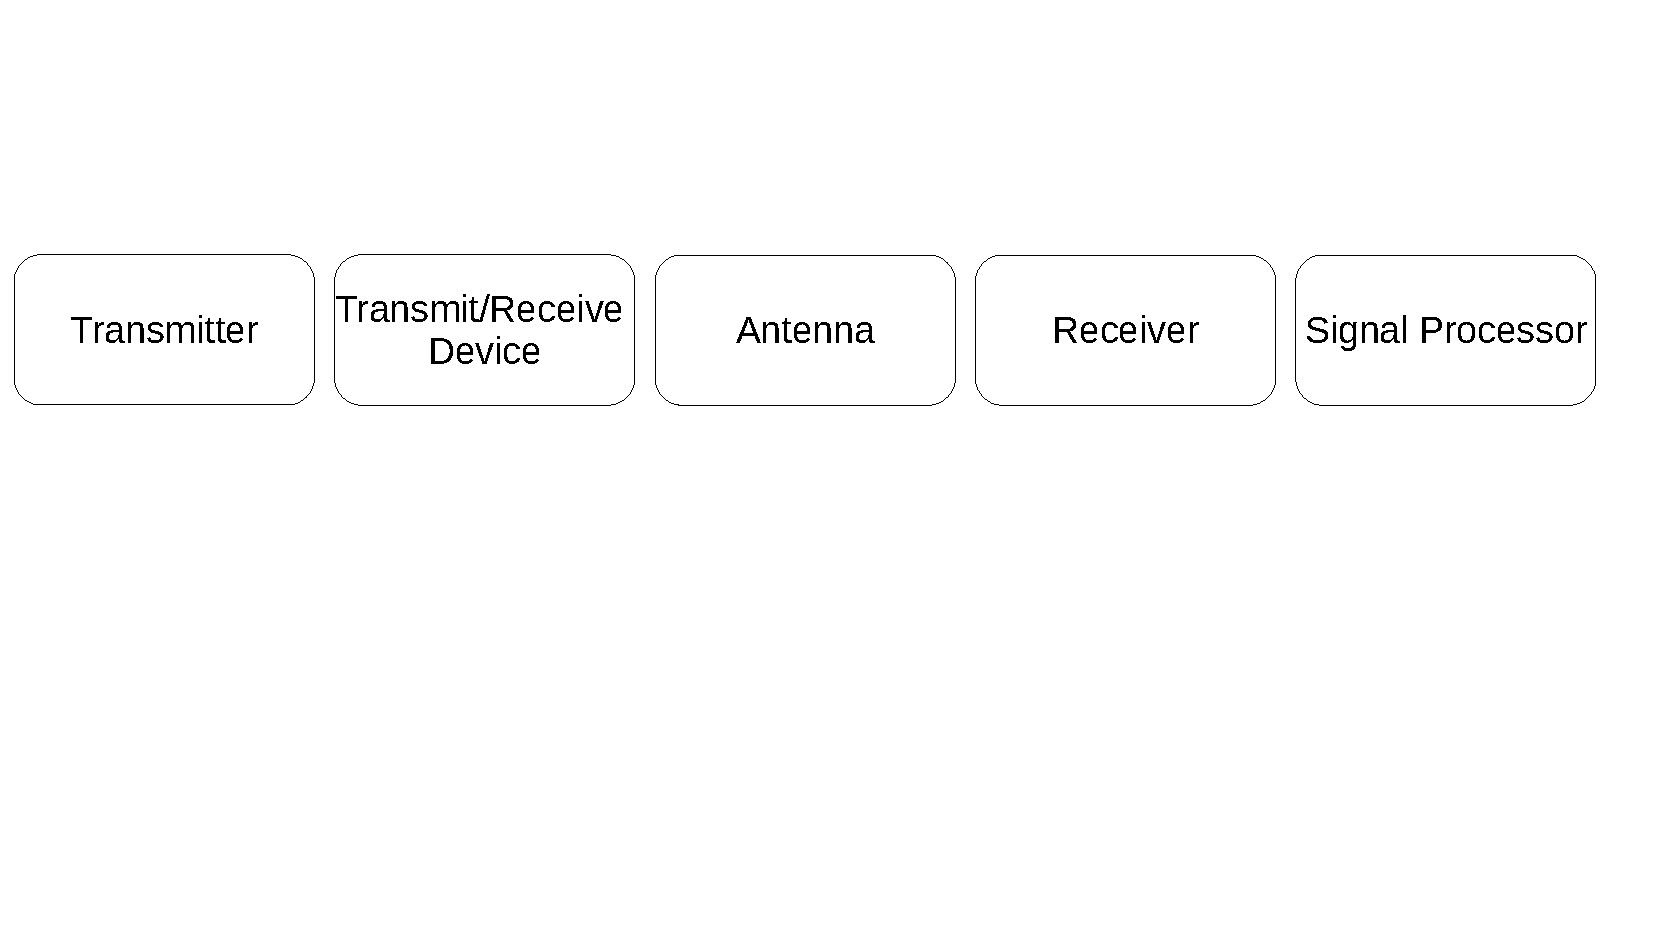
\includegraphics[width=\textwidth]{SystemOverview.pdf}
        \caption{System Overview}
        \label{fig:SystemOverview}    
    \end{figure}
\end{center}

These components perform the major tasks of the system, they are each discussed in detail in their own sections, however, before that can take place, these components are used to perform a specific action in order to detect the space debris, sections~\ref{sec:OptimalFrequency}, \ref{sec:AntennaArray}, \ref{sec:ContinuousWaveandPulsedWave}, \ref{sec:RadarTheoryOfOperation}, and \ref{sec:PulsingCharacteristics} introduce the theory behind the operation of this system. The choices for these sections are directly linked to the type of devices and components seen in Fig.~\ref{fig:SystemOverview}.
The first highly important parameter of the system is the frequency at which it will operate as this is dependent on a number of factors. This is discussed in section~\ref{sec:OptimalFrequency}.


\section{Optimal Frequency} \label{sec:OptimalFrequency}
A number of constraints exist for the frequency of operation of the system, these range from economical, political, technical, and physical. These constraints and the reasons behind the final choice of frequency are discussed within this section.

\subsection{Technical and Physical Limitations} \label{sec:TechnicalandPhysicalLimitations}
The first limitation of the system is the fact that the ionosphere attenuates frequencies from specific frequency ranges. There are two frequency windows at which EM waves penetrate the ionosphere without excessive attenuation \cite{ObjectInformation}.
These frequency windows have a high transmission coefficient for frequencies from the $1~cm$ to $1~m$ wavelength range; these frequency bands are highly useful for transmitting EM waves through the Earths atmosphere as the attenuation is low \cite{frequencyAttenuation}. Frequencies outside of this window (with a few exceptions to the visible light spectrum), are closed due to ionospheric attenuations and reflections (at larger wavelengths) and also attenuate due to resonances created by molecules in the atmosphere (at lower wavelengths) \cite{frequencyAttenuation}.  
If the wavelength of the EM wave is within the bands above, then the attenuation can be considered negligible \cite{ionosphereAttenuationStandard}, \cite[p.~15,124]{radarHandbook}. It is apparent that frequencies within this range provide a negligible attenuation of less than $10^{-3}~db/km$.
Based on these assumptions, the optimal frequency band lies within the $200~MHz$ up to $1~GHz$. %; after $1~GHz$, the atmospheric losses increase accordingly.

The elevation angle of the system is also a contributing factor to the loss of the system as this determines the \textit{volume} of atmosphere that the EM waves travel through to reach the target. Increasing elevation angles result in lower two-way losses, implying that if the system directs its beam directly upwards (towards the zenith), it will have the lowest loss per unit distance \cite[p.~70]{elevationLoss}. This is highly beneficial for the system as it is normally directed upwards and has a FOV that does not greatly increase the \textit{volume} of atmosphere the EM wave has to encounter.


Included in this technical choice is that of currently implemented systems. Many of these operate within the $400 MHz$ to $500 MHz$ frequency bands.
The amount of electrical power required for these systems can often be in the megawatt range and components capable of supplying this power in the $GHz$ range become prohibitively expensive, this further backs up the choice for a lower frequency.

The frequency that is transmitted from the radar is likely to be different to the frequency that is returned by the object, this is in part due to the Doppler shift phenomenon. The maximum frequency shift created by the Doppler shift is evaluated with the use of equation~\ref{eqn:Doppler}. This implies that the maximum expected Doppler frequency shift is unlikely to exceed $\sim~50~kHz$ based on this equation and the estimates of the maximum linear velocity. This value is created on the assumption that the frequency is $1~GHz$ which is the upper bound of frequencies that can be selected from.
\begin{equation} \label{eqn:Doppler}
    f_{d} = \pm \frac{2 v_{r}}{\lambda}    
\end{equation}
Where:
\begin{itemize}
    \item $f_{d}$ is the frequency shift due to the maximum linear velocity of an object
    \item $v_{r}$ is the maximum linear velocity of an object
    \item $\lambda$ represents the wavelength of the frequency of choice.
\end{itemize}
This assumed Doppler shift implies that the frequency bandwidth should accommodate at least $100~kHz$ on either side of the centre frequency.
The Doppler frequency shift of the designed system is discussed in more detail in section~\ref{sec:SNR} where further analysis on the required bandwidth is also analysed as it is dependent on a number of factors.

The frequency choice is highly dependent on the locality of the system and the current frequency usage by other parties as well as population density and frequency usage, which leads to the analysis in section~\ref{sec:PoliticalandEconomicalLimitations}.


\subsection{Characteristics of Frequency}
Based on the frequency choice discussed in section~\ref{sec:PoloticalandEconomicalLimitations} it is clear that the optimal frequency band is the $606~-~614~MHz$ band; a number of parameters are estimated and illustrated in table~\ref{tab:FrequencyDetails}.

\begin{table}
    \caption{Frequency Details}
    \label{tab:FrequencyDetails}
    \begin{center}
        \begin{tabular}{p{70mm}cp{70mm}}
            \hline 
            Parameter & Value \\
            \hline
            Frequency Band & $606~-~614~MHz$ \\
            Center Frequency & $610~MHz$ \\
            Wavelength & $0.4918~m$ \\
            $\lambda /4$ wavelength & $0.12295~m$ \\
            $\lambda /2$ wavelength & $0.2459~m$ \\
            $3 \lambda /4$ wavelength & $0.3689~m$ \\                
        \end{tabular}

    \end{center}
\end{table}
The wavelengths generated within this table are based on the centre frequency of the frequency band. This becomes the primary operating frequency of the system.



\section{Basic Operation} \label{sec:BasicOperation}
The first important characteristic of a radar system is the ability to measure the distance of a target from the observation point. This is undertaken with the simple calculation of the amount of time that it takes a signal to travel from the transmitter to the target and back again, this is evaluated with the use of equation~\ref{eqn:RadarRangeEquation}. This equation evaluates the distance of the target ($R$) by making use of the speed of light (the speed that the EM wave travels, $c$), and the amount of time that it took the signal to travel to the target and back again ($\Delta$).

\begin{equation} \label{eqn:RadarRangeEquation}
    R = \frac{c \Delta T}{2}
\end{equation}
This allows for the calculation for the maximum and minimum round trip times for specific placements of objects from the observer. Table~\ref{tab:RadarRangeValues} illustrates the important round trip times which pertain to this system.

\begin{table}[htb]
    \caption{Radar Range Round Trip Times}
    \label{tab:RadarRangeValues}
    \begin{center}
        \begin{tabular}{p{70mm}cp{70mm}}
            \hline 
            Round Trip Time Parameter & Time (ms) \\
            \hline
            Minimum Distance (Zenith direction) & $1.067$ \\
            Maximum Distance  (Zenith direction & $13.34$ \\
            Maximum Slant Distance & $14.83$ \\
            \hline
        \end{tabular}
    \end{center}
\end{table}
These values take the assumption that the system is capable of steering up to $30^{\circ}$ from the zenith direction. If the system were to steer further, then the maximum slant distance would increase accordingly. The maximum steering ability of the system designed is capable of reaching approximately $50^{\circ}$, however, the maximum slant allowed is reduced in order to increase the reliability of the system. This is discussed in more detail in section~\ref{sec:AntennaArray} as grating lobes can appear when steered past designed levels.

Based on the maximum slant distance round trip time ($14.83 ms$), this places a number of limitations on the system which relate to the pulse repetition frequency, the minimum distance round trip time ($1.067 ms$), limits the pulse width that the system can transmit over. This also creates a limit on the bandwidth of the system as the bandwidth is related to this parameter by $B = 1/ \tau$.
% , however the bandwidth of the system is related to a number of characteristics which are discussed in section~\ref{sec:SNR}***.


The next step in the evaluation of the power that is required to be transmitted onto the object in order to reliably detect it. This begins with the radar range equation.

\subsection{Power Density} \label{sec:PowerDensity}

The first equation defines the power that is incident on the target, this is given by equation \ref{eqn:IncidentPower}. This power is generated with the use of the antenna array, the details of this array are discussed in section~\ref{sec:AntennaArray}, and the creation of the array requires the use of this equation. 

\begin{equation} \label{eqn:IncidentPower}
P_{inc} = P_t * \frac{G_{t}}{4 * pi * R^2} [W/m^2]
\end{equation}

Where:
\begin{itemize}
    \item $P_{inc}$ is the power incident on the target
    \item $P_t$ is the power transmitted from the system
    \item $G_t$ is the gain of the system
    \item $R$ is the distance from the system to the target
\end{itemize}

This equation assumes the use of a directional antenna (not isotropic) which has a corresponding gain. This allows for the concentration of the beam in a specific direction.

The next stage is to determine the magnitude of energy that is reflected by the target, as assumed in section~\ref{sec:SpaceDebrisPhysicalCharacteristics}, the radar cross section of the target is defined and known. 

Equation~\ref{eqn:ReflectedPower} indicates the magnitude of power reflected by this object.

\begin{equation} \label{eqn:ReflectedPower}
P_{refl} = \frac{P_{t} G_{t} \sigma}{4 pi R^2}
\end{equation}

Where:
\begin{itemize}
    \item $P_{refl}$ is the reflected power from the target
    \item $\sigma$ is the radar cross section (RCS) of the target measured in square meters ($m^2$)
\end{itemize}

This reflected power from the target is then received by the system and this is defined by equation \ref{eqn:ReceivedPower}.

\begin{equation} \label{eqn:ReceivedPower}
P_{r} = \frac{P_{t} G_{t} G_{r} \lambda^2 \sigma}{(4 pi )^3 R^4}
\end{equation}

Where:
\begin{itemize}
    \item $P_{r}$ is the received power at the system
    \item $A_{e}$ is the effective aperture of the system
    \item $\lambda$ is the wavelength of the system
    \item $G_{r}$ is the gain of the receive antenna
\end{itemize}

It is assumed that the gain is determined with equation \ref{eqn:Gain}.

\begin{equation} \label{eqn:Gain}
G = \frac{4 pi \eta_{a} A}{\lambda^2} = \frac{4 pi A_{e}}{\lambda^2}
\end{equation}

Where $\eta_{a}$ is the efficiency of the antenna created which is commonly between 0.5 and 0.8 \cite[p.~64]{radarHandbook}.

In the case of the monostatic antenna array, the transmitting and receiving gain are the same as it is the same array. This implies that for bistatic systems, it is possible to have two different ranges for receiving and transmitting \cite[p.~64]{radarHandbook}.


At this point it is pertinent to provide an analysis into the losses that can possibly appear throughout the system, these losses are required before the antenna and antenna array can be simulated. These losses are discussed in section~\ref{sec:SNR}.



\subsection{Pulsing Characteristics} \label{sec:PulsingCharacteristics}
In order to calculate a number of characteristics on the SNR of the system, the pulsing characteristics are required. Fig.~\ref{fig:Pulsing} illustrates the method in which the EM waves are sent out with respect to time. 


\begin{figure}[htb]
    \centering
    \begin{subfigure}{.5\textwidth}
        \centering
            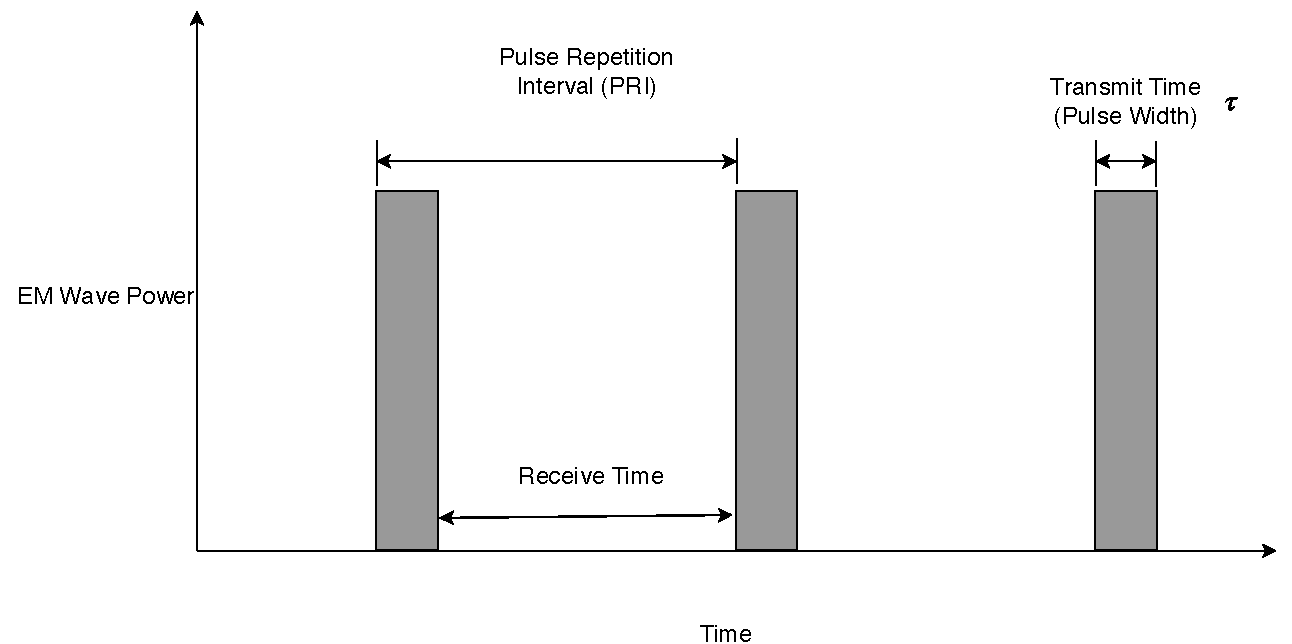
\includegraphics[width=0.9\linewidth]{Pulsing.pdf}
            \caption{Radar EM Wave Pulse}
            \label{fig:Pulsing}
        \end{subfigure}%
        \begin{subfigure}{.5\textwidth}
            \centering
            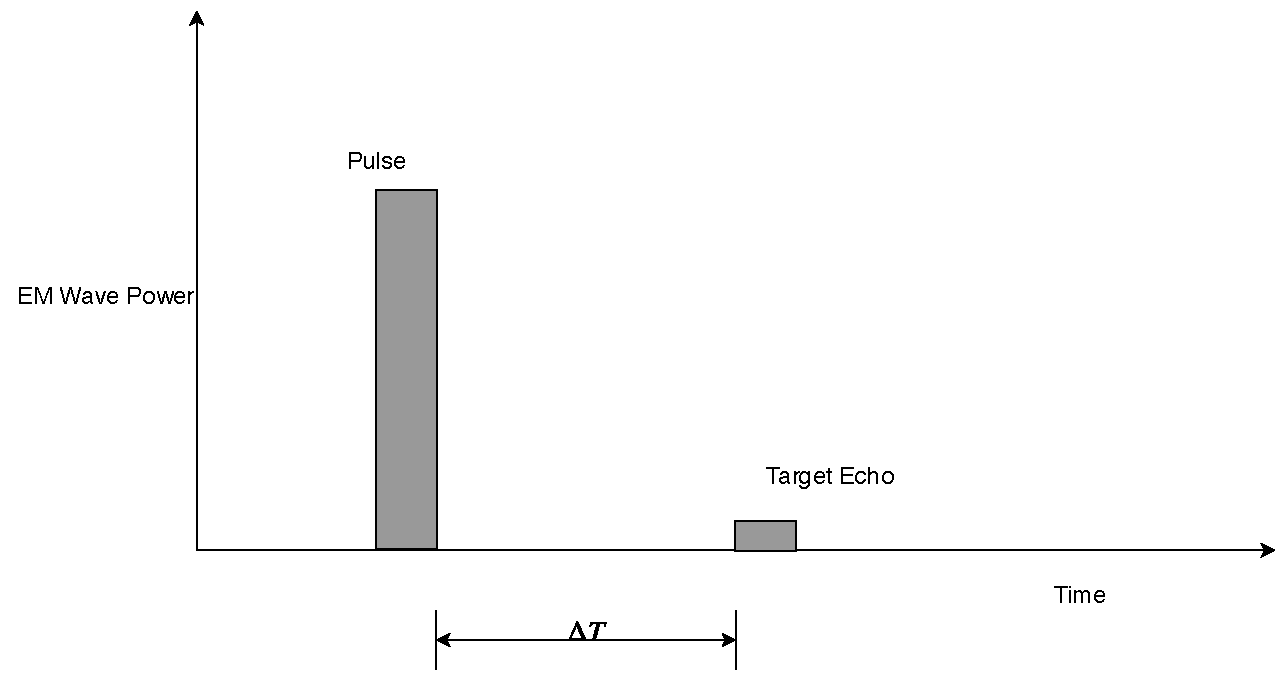
\includegraphics[width=0.9\linewidth]{ObjectDetection.pdf}
            \caption{Object Detection}
                \label{fig:ObjectDetection}
            \end{subfigure}
\caption{Radar Functions}
\label{fig:RadarFunctions}
\end{figure}



This image illustrates a number of important parameters than can be applied to the system at this point in time. These parameters are related to section~\ref{sec:BasicOperation} and more importantly, table~\ref{tab:RadarRangeValues}. This implies that the maximum pulse width must be less than $1.067 ms$, the actual pulse width is likely to take a value far less than this. 
The next parameter is the pulse repetition interval, this is related to the maximum round trip time that a signal can take, which implies that the minimum pulse repetition interval should be greater than $14.83 ms$. This limits the pulse repetition frequency of the system which is defined as $PRF = 1/PRI$, which limits the pulse repetition frequency to $67 Hz$. This is the maximum frequency the system can sustain without limiting the radar range abilities.

Fig.~\ref{fig:ObjectDetection} represents a case where a pulse is sent outwards and is then followed by, a period of time later, a corresponding echo pulse.
The period between the pulse and the echo can be used to determine the altitude that the object has. This illustrates a circumstance of the system detecting an object. 


In order to detect the pulse, the time between each sample (sampling by the ADC) should be no less than the pulse width of the transmitter, this is a minimum requirement for the sampling frequency of the receiver subsystem.

There are cases where large objects, further out than the maximum slant distance will return a signal (the large RCS results in a larger reflection of EM energy), this signal will be returned after the next pulse has occurred and depending on how far the away the object is, the system can read this as an object that appears to be closer than the actual object. This results in an incorrect reading. These cases should be accounted for within the system such that they are kept to a minimum. In most cases this is not an issue as the object is required to be much larger in RCS for it to be detected. More cases are ruled out as these echoes will appear at the antenna while the second pulse is still being transmitted, which implies that the receiver is still deactivated. ***
This phenomenon is known as range ambiguity \cite[p.~22]{radarHandbook}
The parameters defined in this section are evaluated and analysed in section~\ref{sec:Resolution}.

\subsection{Resolution} \label{sec:Resolution}
The resolution of the system is made up of three major parameters: range, angle, or/and Doppler frequency. These three parameters highlight the ability for the system to make a distinction between two objects with differing parameters.

The first of these, the range resolution, is the parameter which defines the ability of the system to make an  effective distinction between two targets that are placed differing distances away from the observation point. It is related to the pulse width of the system as illustrated via equation~\ref{eqn:RangeResolution}. In order to decide on the pulse width required for the system to function, the criteria for the resolution of the range is required.

\begin{equation} \label{eqn:RangeResolution}
\Delta R = \frac{c \tau}{2}
\end{equation}

The limits on the range resolution are coupled with the limits of the bandwidth allowed by the frequency band. The pulse width is related to the bandwidth by the equation $\tau = 1/ B$.
The bandwidth allocated to the frequency band is set at $8 MHz$, which results in a minimum pulse width of approximately $0.125 \mu s$, which is relatively small when compared to alternative systems \cite{AMISR, EISCAT, SIMO, telescope, BeamForming, OrbitDetermination, PlanarArray}. The bandwidth required by the maximum Doppler frequency shift of $50 kHz$, which results in a pulse width of $20 \mu s$.
Lastly, the next parameter which determines the magnitude of the pulse width is the fact that the pulse width cannot be larger than the minimum round trip time (as discussed above) of $1.067 ms$. 
This means that the pulse width can be sized with the $0.125 \mu s - 1.067 ms$ time span.
These limits provide a range resolution of $18.75 m$ and $160.1 km$. Increasing the pulse length will result in a higher SNR, however, then the range resolution suffers.
Based on this evidence, and current implementations of the system, the pulse width of the system is chosen to be $10\mu~s$. This provides enough time for the transmitter to deactivate, and the receiver to activate to listen to the targets echoes, this switching time is required for the system to perform safely, and to avoid the receiver becoming damaged by the transmitter.
This pulse width results in a range resolution of $1.5~km$, which is sufficient considering the number of objects in LEO and the volume that those objects are within. This distance is $0.075~\%$ of the maximum range of the system. The probability of the system detecting two objects within this ambiguous range are unlikely and therefore this is a sufficient assumption.

This pulse width results in a duty cycle which is evaluated with the use of $Duty Cycle = \tau \cdot PRF$, which provides a duty cycle of $675 \cdot 10^{6}$, this is a relatively small duty cycle, implying that the system is using a small amount of energy with respect to its maximum power requirements.
The system constructed should be capable of varying its bandwidth on demand, this provides the ability for the system to scale to meet specific demands. The limits on the pulse width are still present for the detection of space debris, however, this technique can be used to detect smaller debris at the farther distances.

The pulse width is also linked to the SNR of the system through equation~\ref{eqn:SNRPulseWidth}.

\begin{equation} \label{eqn:SNRPulseWidth}
SNR = \frac{P_{t} G_t G_r {\lambda^2} \sigma}{((4 \pi )^3 R^4 k T_s L_s}
\end{equation}

This implies that an increase in pulse width results in an increase in SNR. This is the case based on the fact that the receiver bandwidth is linked to the waveforms bandwidth, this implies that the receivers bandwidth can be substituted for the pulse width in the standard radar range equation \cite[p.~776]{radarHandbook}.
This is a simple method in which to increase the SNR without increasing the cost of the overall system.



\section{SNR} \label{sec:SNR}
The SNR required for this system is highly dependent on the requirements for the probabilities of detection and false alarm. The first simplifying assumption of this section is to assume that the signal received by the object is non-fluctuating, this results in the ability to determine an operational SNR for successful detection \cite[p.~102-103]{radarHandbook}.
The first part of this is to make use of equation~\ref{eqn:SNRProbability} in order to map a selected set of probabilities to a required SNR value \cite[p.~107]{radarHandbook}.

\begin{equation} \label{eqn:SNRProbability}
SNR (dB) = -5 log_{10}N + \Bigg(6.2 + \frac{4.54}{\sqrt{N + 0.44}}\Bigg) log_{10}(A + 0.12 A B + 1.7 B)
\end{equation}

Where 
\begin{equation} \label{eqn:A}
A = ln(\frac{0.62}{P_{FA}})
\end{equation}
and 

\begin{equation} \label{eqn:B}
B = ln \Bigg( \frac{P_D}{1 - P_D} \Bigg)
\end{equation}

This set of equations is used to generate Fig.~\ref{fig:SNRRequired} (in this case $N$ is the number of pulses, which is assumed to be 1).

\begin{center}
    \begin{figure}
        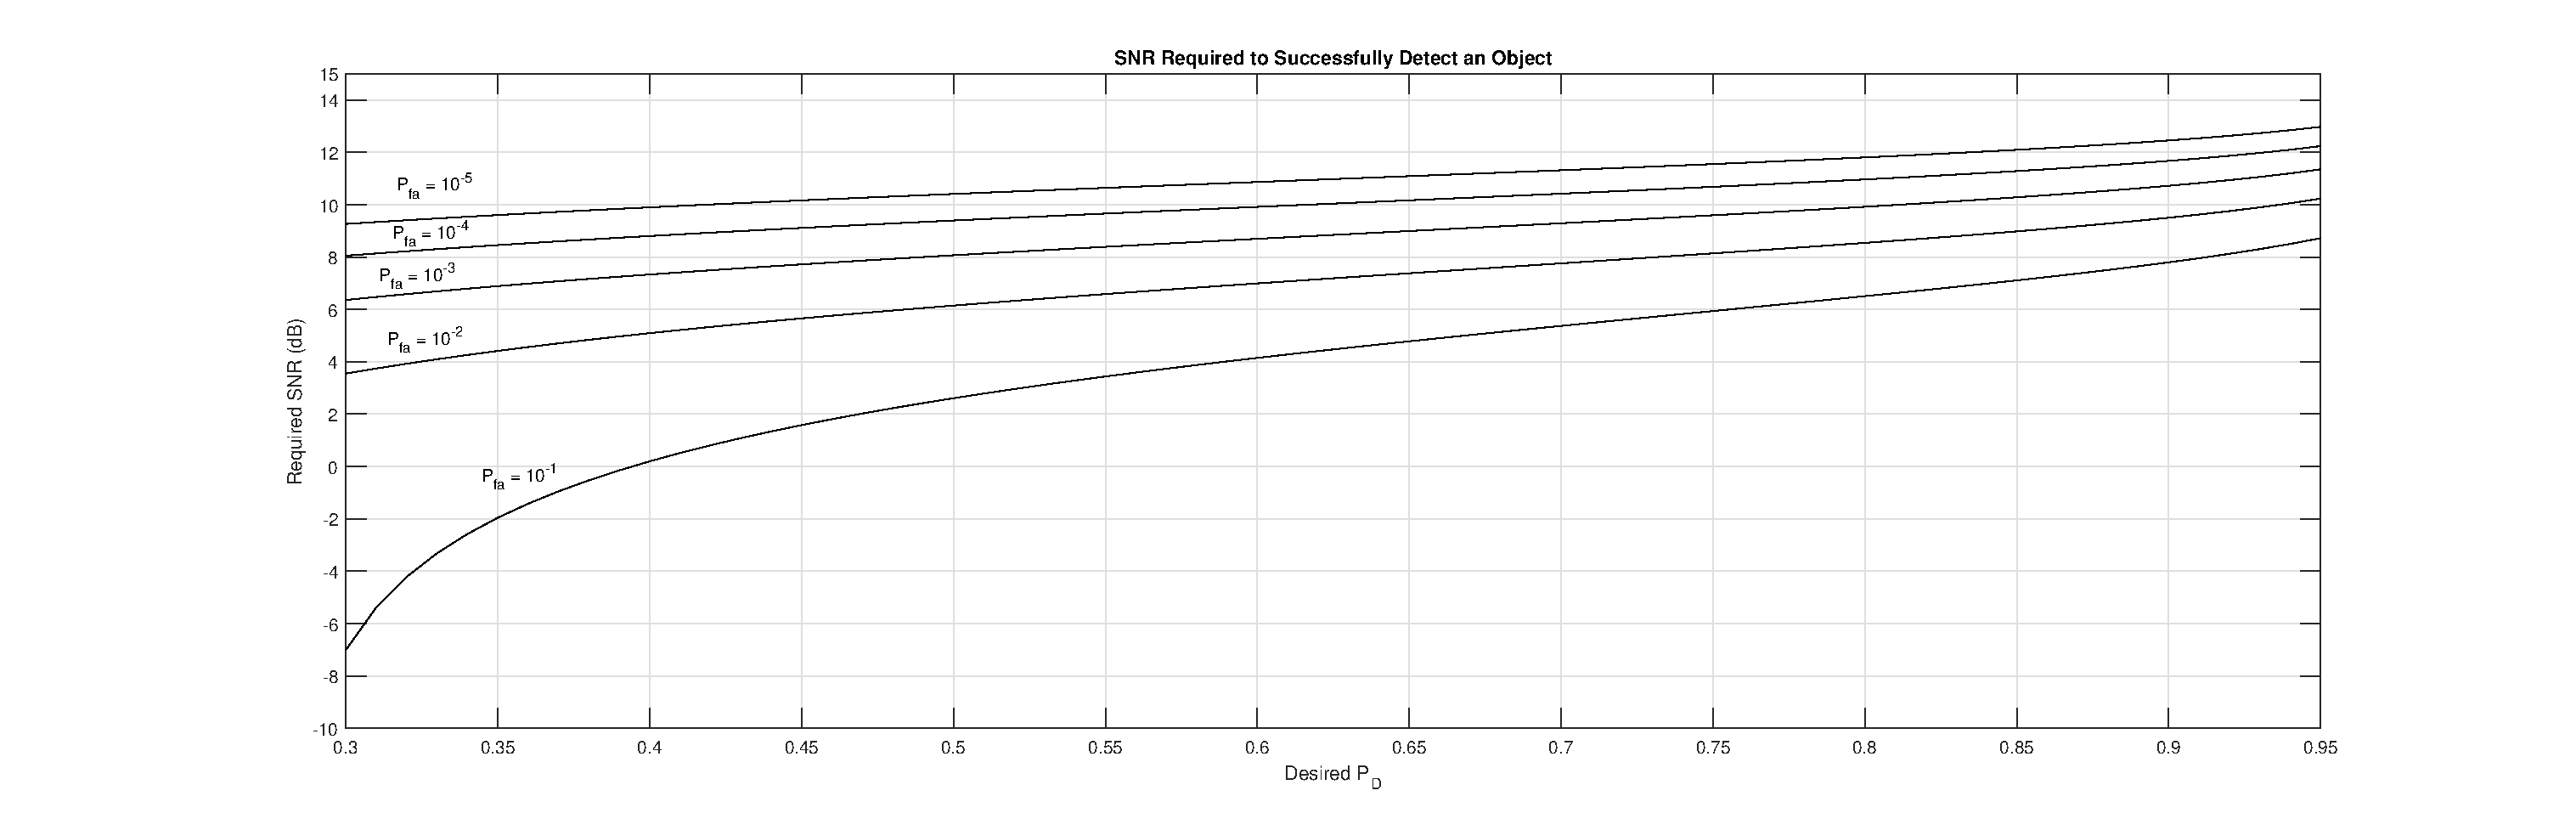
\includegraphics[width=\textwidth]{ProbabilityDetection.eps}
        \caption{SNR Required for Detection}
        \label{fig:SNRRequired}    
    \end{figure}
\end{center}

This implies that in the case that for realistic values for the two probabilities, the SNR required reaches a value of approximately $10 dB$.
This is therefore defined as the minimum SNR ($SNR_{min}$) required for the system to function.
Based on this equation, it can be seen that if the number of pulses is increased, then the SNR required will become lower. This current approximation makes use of a single pulse on a target.

% There are a number of alternative methods in which to specify criteria of the system where the system is designed from th in section~\ref{sec:ParameterEstimation} \cite[p.~72]{radarHandbook}

This first estimate for the minimum SNR required is linked to the noise present in the system, the noise of the system is evaluated in sections~\ref{sec:ReceiverNoise} and \ref{sec:ThermalNoise}.

\subsection{Multiple Pulses} \label{sec:MultiplePulses}
The SNR of the system can be improved with the utilization of multiple pulses while the beam is in a certain position. This implies that, if an object enters the field of view of the main beam, based on the HPBW of the system, it will be within the view of the pulse without steering required.
These multiple pulses can be averaged in order to increase the performance of the detection \cite[p.~66]{radarHandbook}. This implies that the system can emit multiple pulses, where each pulse increases the SNR achieved for a fixed angular position.
The increase in SNR is illustrated in the implementation into the RRE as it has a direct affect on the SNR, this is shown in equation~\ref{eqn:MultiplePulses}.

\begin{equation} \label{eqn:MultiplePulses}
SNR_c (N) = \frac{P_{t} G_{t} G_{r} \lambda^2 \sigma n_p}{(4 pi)^3 R^4 k T_0 F B}  
\end{equation}
The value of $n_p$ represents the number of pulses. The minimum number of pulses possible by this system can be determined with the use of equation~\ref{eqn:ObservableTime} by using the minimum distance an object can be detected (as this is the minimum amount of time an object will be within the HPBW). This estimate results in a time of $0.933~s$. This implies that, based on the PRI of $14.83~ms$, the maximum number of pulses that can be used will be less than $62$ pulses.
In order to account for \textit{dead time} a pragmatic value for this can be estimated to be $50$ pulses. This effect is incorporated in section~\ref{eqn:SNR} and \ref{eqn:RequiredParameters}.

\subsection{Receiver Noise} \label{sec:ReceiverNoise}
The three major losses within any system is made up of the transmitter, receiver, and signal-processing losses.
Of these, the receivers noise is mostly made up of the noise generated by the primary Low Noise Amplifier (LNA) or mixer (if present) \cite[p.~405]{radarHandbook}.
This receiver noise is generated by the phenomenon known as thermal noise, this is discussed in section~\ref{sec:ThermalNoise}.

\subsection{Thermal Noise} \label{sec:ThermalNoise}
The noise from the environment is mostly made up by solar effects. This case deals specifically with the noise generated by the sun. This can contribute to large amounts of noise within the signal if the antenna array is pointed in the direction of the sun, however, great care should be taken to avoid pointing the antenna array directly at the sun. There will still be a small contribution of the suns noise from the sidelobes of the antenna array, however, this power is greatly reduced.

The second source of noise, the largest component within the system, is that generated by the receiver electronics.
Thermal noise power, being uniform over the frequency spectrum contributes to the noise power over the bandwidth of the system. This implies that the thermal noise power is directly proportional to the receivers bandwidth. This power is determined with the use of equation~\ref{eqn:ThermalNoise}.

\begin{equation} \label{eqn:ThermalNoise}
P_{n} = k T_{s} B = k T_{0} F B
\end{equation}

Where:
\begin{itemize}
    \item $k$ is Boltzmann's constant ($1.38 \cdot 10^{-23} Watt-sec/K$)
    \item $T_{0}$ is the standard temperature (normally $290 K$)
    \item $T_{s}$ is the system noise temperature ($T_{s} = T_{0} F$)
    \item $B$ is the receivers bandwidth ($Hz$)
    \item $F$ is the noise figure of the receiver subsystem.
\end{itemize}

The noise figure defined here should be given in real amplitude (convert from $dB$ as this is what it is defined as). The bandwidth defined here is a calculated value and is dependent on two factors of the system. Typical noise figures for LNA's range from $2.5 - 5 dB$, the value used for this calculation is taken to be $2.5 dB$.
% The first of these can be defined with the use of the largest doppler frequency shift detectable by the system. This is defined in \ref{sec:TechnicalandPhysicalLimitations} with the introduction of the debris characteristics.

% The second of these is defined by the minimum pulse width of the signal. This is calculated in section~\ref{sec:Resolution}. 
% This second case is highly important because if the bandwidth of the receiver is made smaller than the bandwidth required for the pulse width, then the power on the target will be reduced and this will cause inconsistencies and will reduce the range resolution of the system \cite[p.~65]{radarHandbook}. If the bandwidth of the receiver is created to be larger than the reciprocal of the pulse width, then the SNR of the system will decrease. This implies that the bandwidth of the receiver can occupy a small frequency band which is set by the pulse width. This implies that if the pulse width of the system is set to 1us, then the bandwidth of the system is 1 MHz.
% The approximation of using $1/\tau$ is often used in monostatic systems \cite[p.~65]{radarHandbook}.


At this point it is possible to evaluate the required parameters of the system with the use of the noise figure that is estimated above.
The SNR is defined by equation~\ref{eqn:SNR}.

\begin{equation} \label{eqn:SNR}
SNR = \frac{P_{t} G_{t} G_{r} \lambda^2 \sigma n_p}{(4 pi)^3 R^4 k T_0 F B}
\end{equation}


Rearranging this equation and placing the known value on the right hand side results in equation~\ref{eqn:RequiredParameters}.

\begin{equation} \label{eqn:RequiredParameters}
P_{t} G_{t} G_{r} = \frac{SNR_{min} (4 \pi )^3 R^4 k T_{0} F B}{{\lambda}^2 \sigma n_p} = 
\end{equation}
Where the values on the right hand side of the equation are listed in table~\ref{tab:DesignValues}.
This implies that the product of the variables on the left hand side of the equation are required to be equal to the value on the right hand side for the system to function as designed.

\begin{table}[htb]
    \caption{Major Design Features}
    \label{tab:DesignValues}
    \begin{center}
        \begin{tabular}{p{70mm}cp{70mm}}
            \hline 
            Parameter & Value \\
            \hline
            $SNR_{min}$ & $10 dB$ \\
            $R$ & $2223.8 km$ \\
            $k$ & $1.38064852 \cdot 10^{-23} m^2 kg s^{-2} K^{-1}$ \\
            $T_{0}$ & $K$ \\
            $F$ & $val$ \\
            $B$ & $val$ \\
            $\lambda$ & $val$ \\
            $\sigma$ & $val$ \\
            $n_p$ & $50$ \\
            \hline
        \end{tabular}
    \end{center}
\end{table}


This provides a starting point for the design of the antenna and antenna array such that it can be built to satisfy the requirements thus far.
***

\section{Antenna} \label{sec:Antenna}
The antenna forms the most basic unit of the system. It is responsible for transforming an electrical signal into an EM wave and directing that EM energy into a specific direction. It is also important as it makes use of its reciprocity such that it can receive and transmit with the same characteristics. This makes it ideally suited to this application as it can be used to transmit the EM wave and receive the wave, thus reducing the cost and complexity of the system.
The antenna, and corresponding array is designed here to satisfy the requirements in equation~\ref{eqn:RequiredParameters}, these parameters are the systems gain and the power that the system is required to sustain.

The most important design requirement of the antenna is that is should have sufficient gain, it should be able to direct its energy in a specific direction. The second component of the antenna is that it should be capable of sending out this EM wave and receiving the echo with minimal losses throughout the process. This implies that it is designed to be as efficient as possible.
The array, discussed in section~\ref{sec:AntennaArray} discusses the design of multiple antennas and their interconnectedness such that the system can benefit from multiple antennas working together.

The first design decision is that of the type of antenna to make use of. The design methodology for this has the following criteria: cost, construction, bandwidth, sidelobes, gain, efficiency, power capabilities, durability, polarization (and the Axial Ratio), VSWR, etc. 
These parameters of the antenna are discussed below and the design is drawn up based on these criteria.

The first part of the design process for the antenna is to determine a simplistic antenna that allows for easy construction while also providing the required EM wave characteristics.
The first important characteristic of the system to consider is to analyse the polarization of EM waves as they enter progress through the ionosphere and how they are affected by the reflection off of the target.

The choice of antenna is a crossed-dipole antenna, the following sections are used to illustrate the process used to determine the correct antenna and how its characteristics were designed and calculated.

\subsection{Polarization} \label{sec:Polarization}
There are four commonly used polarizations that are used in antennas: vertical, horizontal, right hand circular, and left hand circular, these are created based on the geometry of the antenna and how it is fed.
EM waves entering the ionosphere experience Faraday Rotation, this implies that in the case that a linearly polarized wave passes through the ionosphere, its polarization is rotated from the interaction with the Earth's magnetic field. This interaction is highly dependent on the frequency of the signal and a number of other factors \cite[p.~24]{faradayRotationSlides}, which implies that the rotation of this linear EM wave can rotate through an arbitrary amount of degrees based on the environmental conditions at the time of transmission. This rotation implies that if a linear antenna were to be used, the receiving antenna would be unable to determine how much the reflected wave had rotated and if it cannot match the exact rotation, then this will result in a significant loss of signal (often up to $20 dB$), which can severely impair the system functionality.

In order to overcome this, circular/elliptical polarization can be employed as this is not affected in the same way.
When using circular polarization, the handedness of the polarization swaps. This implies that if left hand polarization is used on the transmitting antenna, when the EM wave reflects off of the target, the polarization swaps to right hand circular.
This results in the requirement for the antenna to be circularly/elliptically polarized, and to have the ability to detect both left and right handed polarization with equation gain magnitudes.
Circularly polarized antennas are used for Earth-to-Space and Space-to-Earth communication because of these effects on the polarization. On top of the circularly polarized EM wave, RHCP is commonly used for transmission \cite[p.~31]{crossedDipoleDesign}.


\subsection{Resonant Frequency and Bandwidth} \label{sec:ResonantFrequencyandBandwidth}
The antenna is designed such that it resonates at the desired frequency ($610 MHz$), which results in the capacitive and inductive effects cancelling each other out, this makes the antenna efficient. During construction of the antenna, there may be inconsistencies with some of the lengths, so tuning of individual antennas may be required such that they function optimally. In order to counteract this, the antenna is constructed such that it is capable of operating over a bandwidth. This bandwidth is specified in section~\ref{sec:SNR}.


\subsection{VSWR and Return Loss} \label{sec:VSRWandReturnLoss}
The Voltage Standing Wave Ratio (VSWR) is an important parameter for any antenna, this is the characteristic which determines the ratio of the input signal which is reflected to what is transmitted. This value should be as low as possible, it ranges from 1 (complete signal transmission) to infinite (complete signal reflection). These correspond to a perfect match and a perfect mismatch respectively.
A VSWR value of lower than $1.3:1$ is sufficient for this application as this represents a return loss of $-17.7 dB$ \cite{AntennaPrice1,AntennaPrice2,AntennaPrice3,AntennaPrice4}. This value is a compromise between cost and antenna performance. Lower VSWR values become difficult to achieve as the price becomes prohibitive. This value is attained based on current implementations of these types of antennas and their specifications.
This VSWR results in a low reflection back into the amplifier (and consequently reflection that doesn't enter the antenna when in receiving mode).

The parameters illustrated above are calculated with the use of equations~\ref{eqn:VSWR}, and \ref{eqn:ReturnLoss}.


\begin{equation} \label{eqn:VSWR}
VSWR = \frac{1 - |\Gamma|}{1 + |\Gamma|}
\end{equation}

\begin{equation} \label{eqn:ReturnLoss}
Return Loss (dB) = -10 log_{10} \Bigg[ \Big(\frac{VSWR - 1}{VSWR + 1} \Big)^2 \Bigg]
\end{equation}
Where the reflection coefficient, $\Gamma = \frac{Z_L - Z_0}{Z_L + Z_0}$ and $Z_L$ is the load impedance and $Z_0$ is the characteristic impedance.

This VSWR value defined here is linked to the bandwidth of the antenna, as this VSWR will not be maintained over a large frequency range. In this case it is useful to define a maximum VSWR over the frequency range of the antenna. The design for this is such that the VSWR is less than $2:1$ for the bandwidth of the antenna (and system as a whole).

\subsection{Axial Ratio} \label{sec:AxialRatio}
The axial ratio defines the shape of the ellipse of the EM wave, the aim is to generate an axial ratio which approaches $0 dB$, and this value should be chosen such that its magnitude is greater than one to create the RHCP \cite[p.~32]{crossedDipoleDesign}.
The important procedure to note here is that the polarization is created with the use of creating a phase delay between the two dipoles of the antenna, this delay is set to $90^{\circ}$. 


\subsection{Antenna Construction} \label{sec:AntennaConstruction}
The physical construction of the antenna is created such that it consists of two half-wavelength dipoles that are aligned at right angles with respect to each other. The currents within these two dipoles have equal magnitude and they are phased $90^{\circ}$ apart. 
Commonly, these crossed-dipole antennas are set up with a reflector such that half of the radiation pattern is reflected in order to double the gain of the antenna \cite[p.~108]{IEEECrossedDipole}. 

Fig.~\ref{fig:Crossed-DipoleGeometry} illustrates the simple geometry of a crossed dipole antenna.

\begin{figure}[htb]
    \centering
    \begin{subfigure}{.3\textwidth}
        \centering
            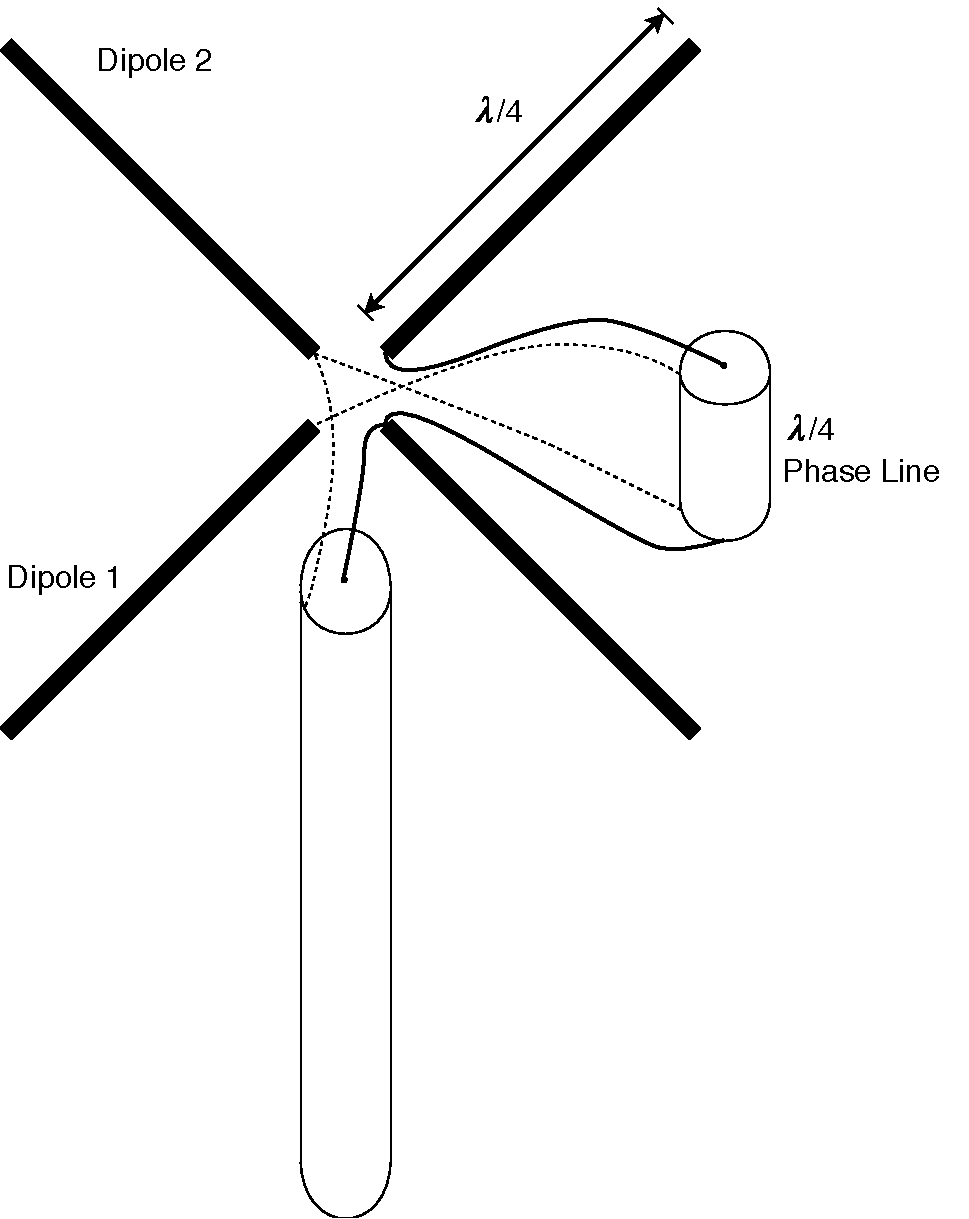
\includegraphics[width=\textwidth]{Crossed-Dipole.pdf}
            \caption{Crossed-Dipole Geometry}
            \label{fig:Crossed-DipoleGeometry} 
        \end{subfigure}%
        \begin{subfigure}{.3\textwidth}
            \centering
            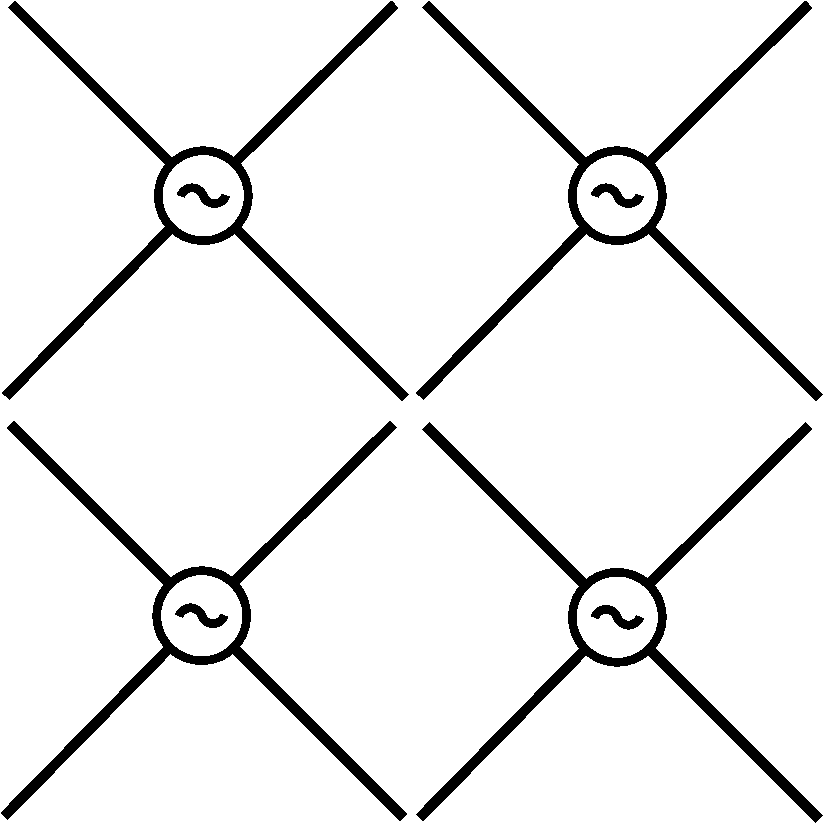
\includegraphics[width=\textwidth]{ArrayGeometry.pdf}
            \caption{Array Geometry}
            \label{fig:ArrayGeometry}  
            \end{subfigure}
\caption{Antenna Construction and Array Layout}
\label{fig:AntennaConstructionArrayLayout}
\end{figure}

The arms of the antenna illustrated here are positioned parallel to the ground. This is done because, in general, it is used to create circularly polarized EM waves in the $\pm z$ directions.

Clearly, based on the requirements of this antenna, the radiation in the $-z$ direction is not required. The implementation of a perfect electrical conductor placed below the antenna will redirect this part of the radiation pattern upwards where it constructively interferes with the radiation patter in the $+z$ direction \cite[p.~110-111]{IEEECrossedDipole}. This ground plane is required to be placed a quarter wavelength above the ground for this mechanism to work. This mechanism is based on image theory such that the system gains a doubling in gain \cite[p.~111]{IEEECrossedDipole}. This structure is created in FEKO and simulated for the selected frequency. The polar plot and cartesian plots for the radiation patterns are illustrated in Fig.~\ref{fig:Crossed-Dipole-Radiation-Patterns}. It is important to note from these plots that the antenna which makes use of the ground plane has a $3~dB$ than the antenna in free space. This implies that the use of a ground plane will increase the performance of each individual antenna without any loss to the ability of the system. The left and right hand circular polarization are not affected by the use of the ground plane either. Based on these simulations a number of characteristics of the two antenna configurations can be compared. This is illustrated in table~\ref{tab:AntennaConfigurations}.

\begin{figure}[htb]
    \centering
    \begin{subfigure}{.5\textwidth}
        \centering
            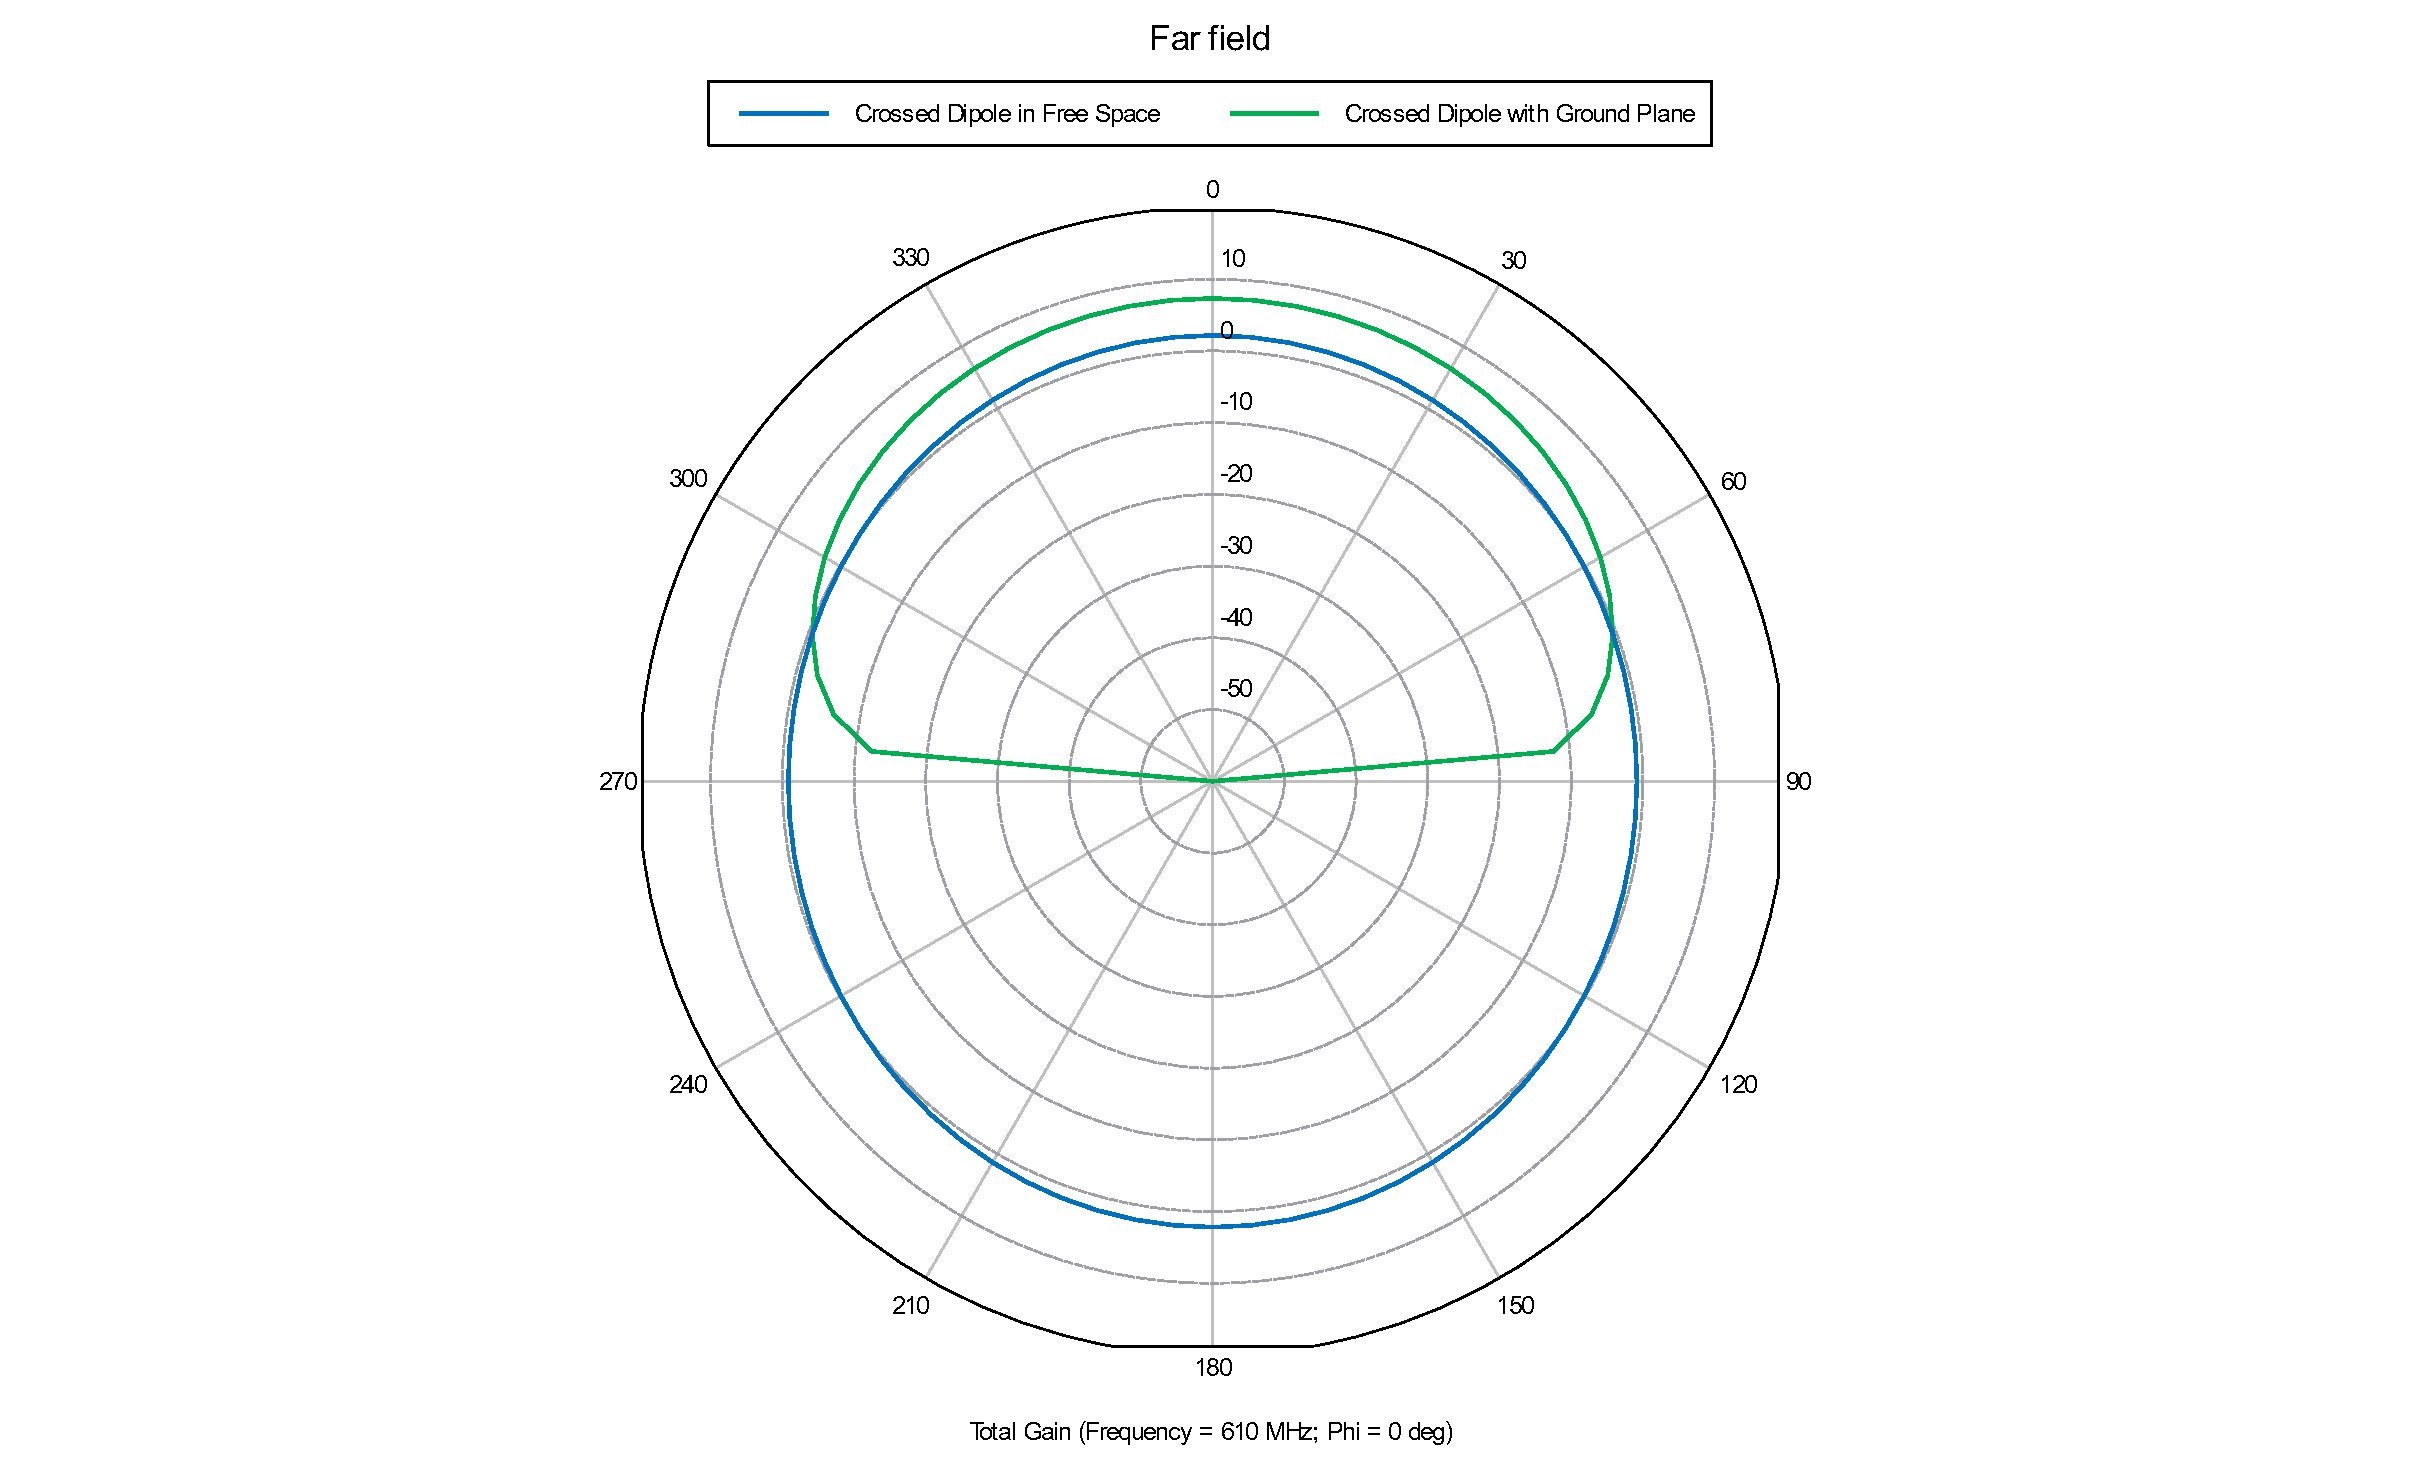
\includegraphics[width=0.9\linewidth]{Crossed-Dipole-Polar-Plot.pdf}
            \caption{Crossed Dipole Polar Plot}
            \label{fig:Crossed-Dipole-Radiation-Patterns-Polar}
        \end{subfigure}%
        \begin{subfigure}{.5\textwidth}
            \centering
            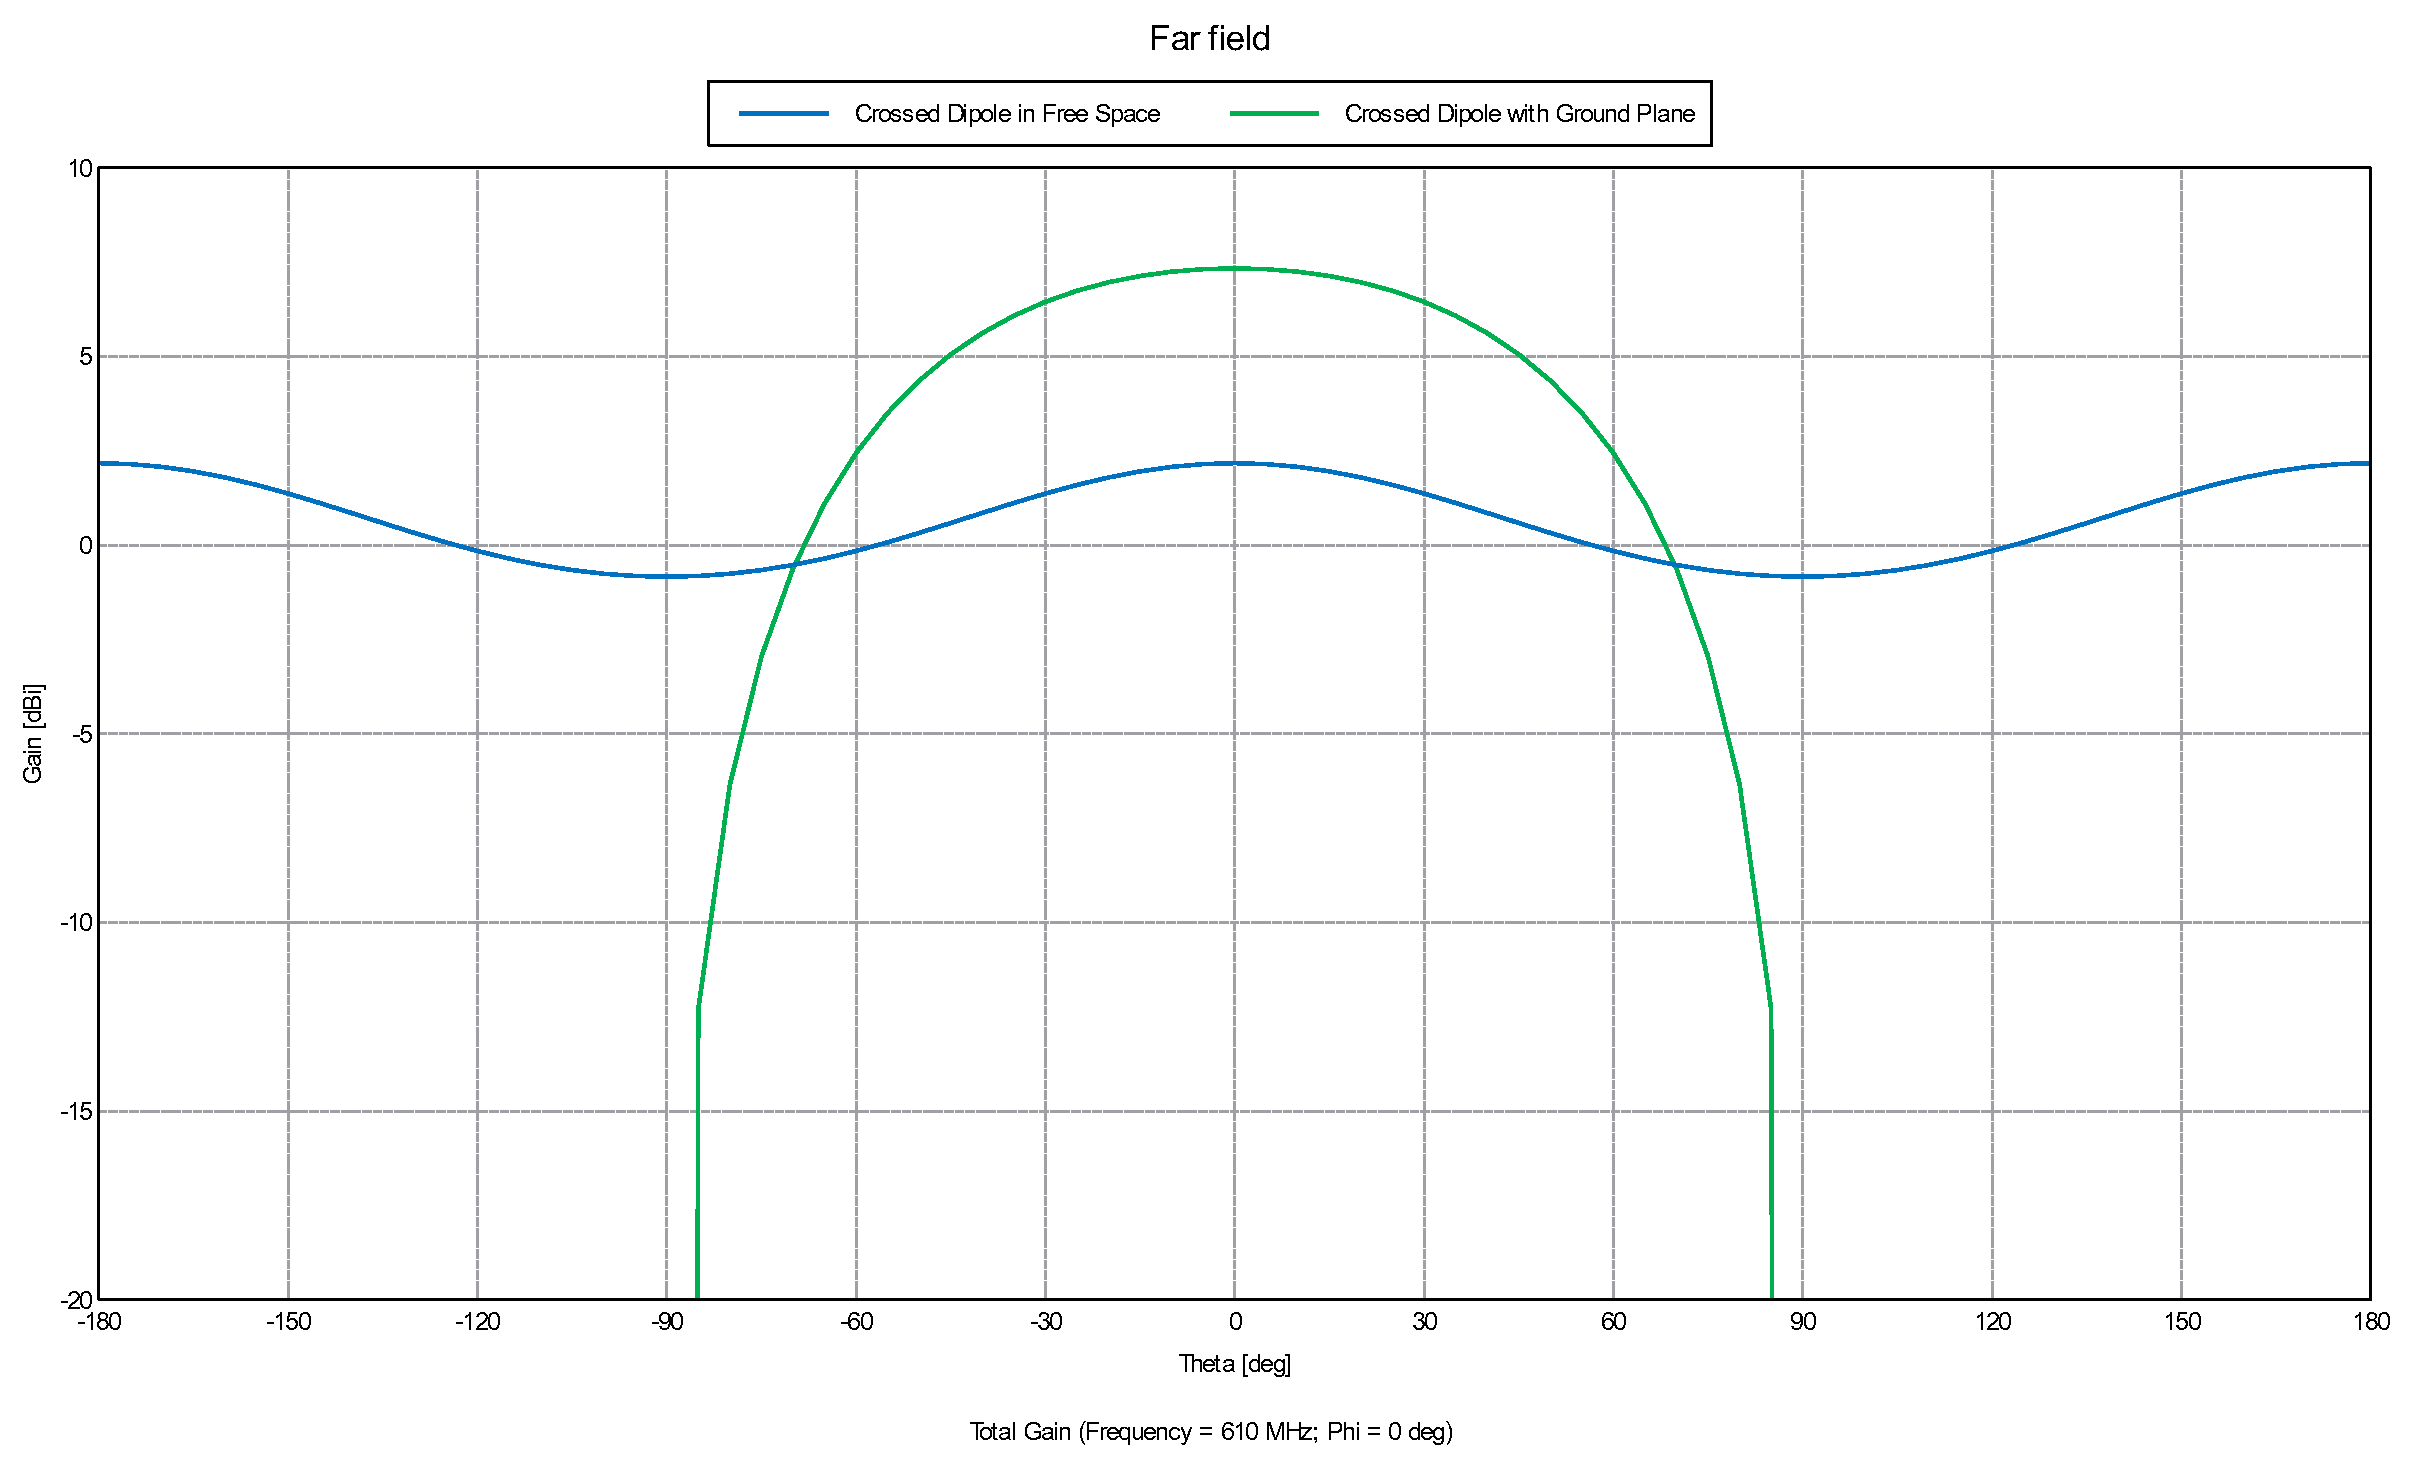
\includegraphics[width=0.9\linewidth]{Crossed-Dipole-Cartesian-Plot.pdf}
            \caption{Crossed Dipole Cartesian Plot}
                \label{fig:Crossed-Dipole-Radiation-Patterns-Cartesian}
            \end{subfigure}
\caption{Crossed Dipole Radiation Patterns}
\label{fig:Crossed-Dipole-Radiation-Patterns}
\end{figure}


\begin{table}[htb]
    \caption{Crossed Dipole Comparison}
    \label{tab:AntennaConfigurations}
    \begin{center}
        \begin{tabular}{p{60mm}cp{40mm}cp{40mm}}
            \hline 
            Parameter & Crossed Dipole (free space) & Crossed Dipole (ground plane) \\
            \hline
            Maximum Gain ($dBi$) & $2.175$ & $7.340$ \\
            Maximum Gain Direction (degrees) & $0$ & $0$ \\
            Minimum Gain ($dBi$) & $-0.835$ & $null$ \\
            Minimum Gain Direction (degrees) & $\pm 90$ & $\pm 90$ \\
            Half Power Beam Width ($-3 dB$) & N/A & $100.401$ \\
            \hline
        \end{tabular}
    \end{center}
\end{table}
Based on the features in table~\ref{tab:AntennaConfigurations}, it is clear that this gain should be multiplied by a large factor in order to meet the requirements stated in section~\ref{sec:ThermalNoise}. This is accomplished with the use of an antenna array, this is discussed in section~\ref{sec:AntennaArray}.
The antenna geometry is highly important as it should be able to withstand a range of environmental conditions that range from extreme temperatures to humidity variations, to high wind speeds.
The ideal material for construction of the antenna is copper as this has the lowest resistivity while having a low cost.
The first important parameter of each of the dipoles is to determine the current density throughout the conductor and therefore to optimize the sizing of the wire such that it takes into account the skin effect.
This is calculated with the use of equation~\ref{eqn:SkinDepth}.

\begin{equation} \label{eqn:SkinDepth}
\delta = \sqrt{\frac{\rho}{\pi \cdot f \cdot \mu}} = 2.6397 \cdot 10^{-6} m
\end{equation}
Where $\rho$ is the resistivity of copper ($1.678 \cdot 10^{-8} \Omega m$) and $\mu$ is the absolute magnetic permeability of the material ($4 \pi \cdot 10^{-7} H/m \cdot 0.999991$).
This value for the skin depth implies that the conductor used should, ideally, be a hollow tube which has a wall thickness that should be larger than the size calculated in equation~\ref{eqn:SkinDepth}. This reduces the cost of each conductor while reducing the weight and therefore the strength of the connectors required.
The added benefit of the hollow conductor tube is that it can be expanded to increase the bandwidth of the antenna. 
The second factor to consider for the thickness of this conductor is related to the power requirements. In order to determine the thickness of this tube, it should be sufficient to dissipate the required amount of power under the maximum temperatures possible in the area. The power that is required to be dissipated by the antenna can be minimized by matching the system, this reduces the losses and hence the power required to be dissipated.


The size of this tube is sized such that it matches up with the maximum required bandwidth of the system as a whole. The larger the radius of this tube the greater bandwidth the antenna can achieve.



\section{Antenna Array} \label{sec:AntennaArray}
The antenna array, constructed with multiple individual antennas work collectively in order to augment the radiation pattern. These antennas, in coordination, create a highly directed radiation pattern with higher gain than the individual antennas. The antennas are dynamically phased and excited such that the radiation pattern changes to match the required pattern to detect the debris.

The criteria of the array can be satisfied with the correct choice of array factor, element separation, phasing, and the excitation of the individual elements.

These are discussed in the following sections.

\subsection{Field of View and Beam Direction} \label{sec:FieldofViewandBeamDirection}
The radiation pattern required, based on the system designed, should be capable of directing the EM wave in the direction of the zenith and be capable of steering $30^{\circ}$ away in all directions.

The radiation pattern required from this array should have a large maximum gain with a small beam width. This is required for the system such that the system can detect objects in the desired range, and to increase the cross-range resolution (the ability to make a distinction between two objects within an angle range).

This requirement is uniquely suited to the use of a broadside array, in which the maximum radiation is directed in the broadside: $\Theta = 0$.
In order to accomplish this, the individual antennas maxima are also required to be directed in this direction. This justifies the implementation of the crossed dipole.
The design of the antenna in the previous section is duplicated for this array, this implies that the sizing of the dipoles are kept the same, the height above the ground plane is kept the same ($\Lambda /4$), and the phase between each dipole keeps the $90^{\circ}$ to create the circular polarization.


In order to accomplish this, the antennas are placed in a grid arrangement such that the array forms an $n \times m$ matrix shape.
The array is then excited such that the main bean is directed towards the zenith. This is accomplished by determining the point at which equation~\ref{eqn:FirstMaximum}
is equal to zero \cite[p.~296]{Balanis}. Where $\Psi$ represents the steering angle of the array, $k = \frac{2 \pi}{\Lambda}$ and $\beta$ represents the progressive phase delay required between each of the elements.

\begin{equation} \label{eqn:FirstMaximum}
\Psi = k d cos \theta + \beta = 0
\end{equation}
This is accomplished by creating a zero phase delay between the elements. This applies to the case of the uniformly excited array, which implies that all elements in the array have the same amplitude excitation.
This achieves the zenith direction gain of the array. The next stage is to determine the optimal spacing between each element.


\subsection{Element Spacing} \label{sec:ElementSpacing}
The second requirement of this broadside radiation is that there should be no other maxima in the radiation pattern, this phenomenon is known as grating lobes.
The presence of side lobes within the radiation pattern is unwanted as this can result in large amounts of radiated energy in unwanted directions. These sidelobes also result in a misuse of the energy that is used in the system.
The reduction of side lobe level is discussed in more detail in section~\ref{sec:ElementExcitation}.


In order to avoid the grating lobes, the separation between each consecutive element in the array should not be multiplies of the wavelength of the antenna \cite[p.~297]{Balanis}.
In order to eliminate this probability, the spacing between elements should be less than one wavelength.



The spacing between each element in the array is set at $\Lambda/2$ which satisfies this criteria.
In order to achieve this spacing, the antennas are rotated by $45^{\circ}$, this allows for tighter packing of the antennas. This configuration is illustrated in Fig.~\ref{fig:ArrayGeometry}, this is for a $2 \times 2$ array, the illustration is from above the array.



This creates a manageable spacing between the elements such that they can be easily installed and will not interfere with adjacent antennas (mechanically). This is also important for cases where antennas need replacing, this makes this process easier.

The elements spaced the same distance above the ground plane as the case for the single antenna. The ground plane is created with a conducting mesh. The mesh is created such that the spacing between each consecutive line is less than $\Lambda/10$ apart. This spacing reduces the cost of the ground mesh as this ground mesh acts as a solid surface in reference to the frequency that is incident upon it.

A secondary method to prevent grating lobes is by specifying the element spacing (not implemented in this solution) where equation equation~\ref{eqn:ElementSpacing} provides the spacing \cite[p.~331]{radarHandbook}. In this case, the maximum steering angle required is the parameter, $\theta$, this results in a spacing that can be approximated by $0.75 \Lambda$. 
This method of spacing the elements can reduce the cost of the overall array as it can result in the reduction of required antenna elements \cite[p.~331]{radarHandbook}.
The reason that this was not used is based on the fact that a large amount of power is input to the system so increasing the number of elements reduces the power experienced by each antenna.

\begin{equation} \label{eqn:ElementSpacing}
d = \leq \frac{\Lambda}{(1 + | sin \theta |)}
\end{equation}


\subsection{Main Beam Gain} \label{sec:MainBeamGain}
The gain of the main beam is highly important to the functionality of the system. This part of the design is created such that the antenna array is sized such that the gain is maximized while maintaining a practical number of elements.
The design procedure for sizing the array is based on a number of factors. The first of these is based on previous implementations of antenna arrays to detect space debris \cite{AMISR}, this made use of an array of $64 \times 64$ elements which creates a total of $4096$ elements.
The second design choice is the fact that this sizing results in the ability to create a modular design with the elements. The sizing of this array is structured such that it is a square shape, this makes the phasing ability the same for both steering directions and creates a relatively uniform steering FOV.
During simulations, the increase in gain between a $64 \times 64$ matrix and a $70 \times 70$ array resulted in an increase of $0.775 dB$, which does not warrant the extra cost for the extra $804$ antennas.
Increasing the number of antennas reduces the power requirement for each antenna as this splits the total power requirement between each antenna.
The next stage is to attempt to steer this main beam in the required directions in order to track the debris. The steering of the system is discussed in section~\ref{sec:ElementPhasing}.
To illustrate this feature of the system, Fig.~\ref{fig:MainBeamGain} shows the differences between a $32 \times 32$, $64 \times 64$, and a $70 \times 70$ array and the different gains they each produce.


\begin{figure}[htb]
    \centering
    \begin{subfigure}{.5\textwidth}
        \centering
            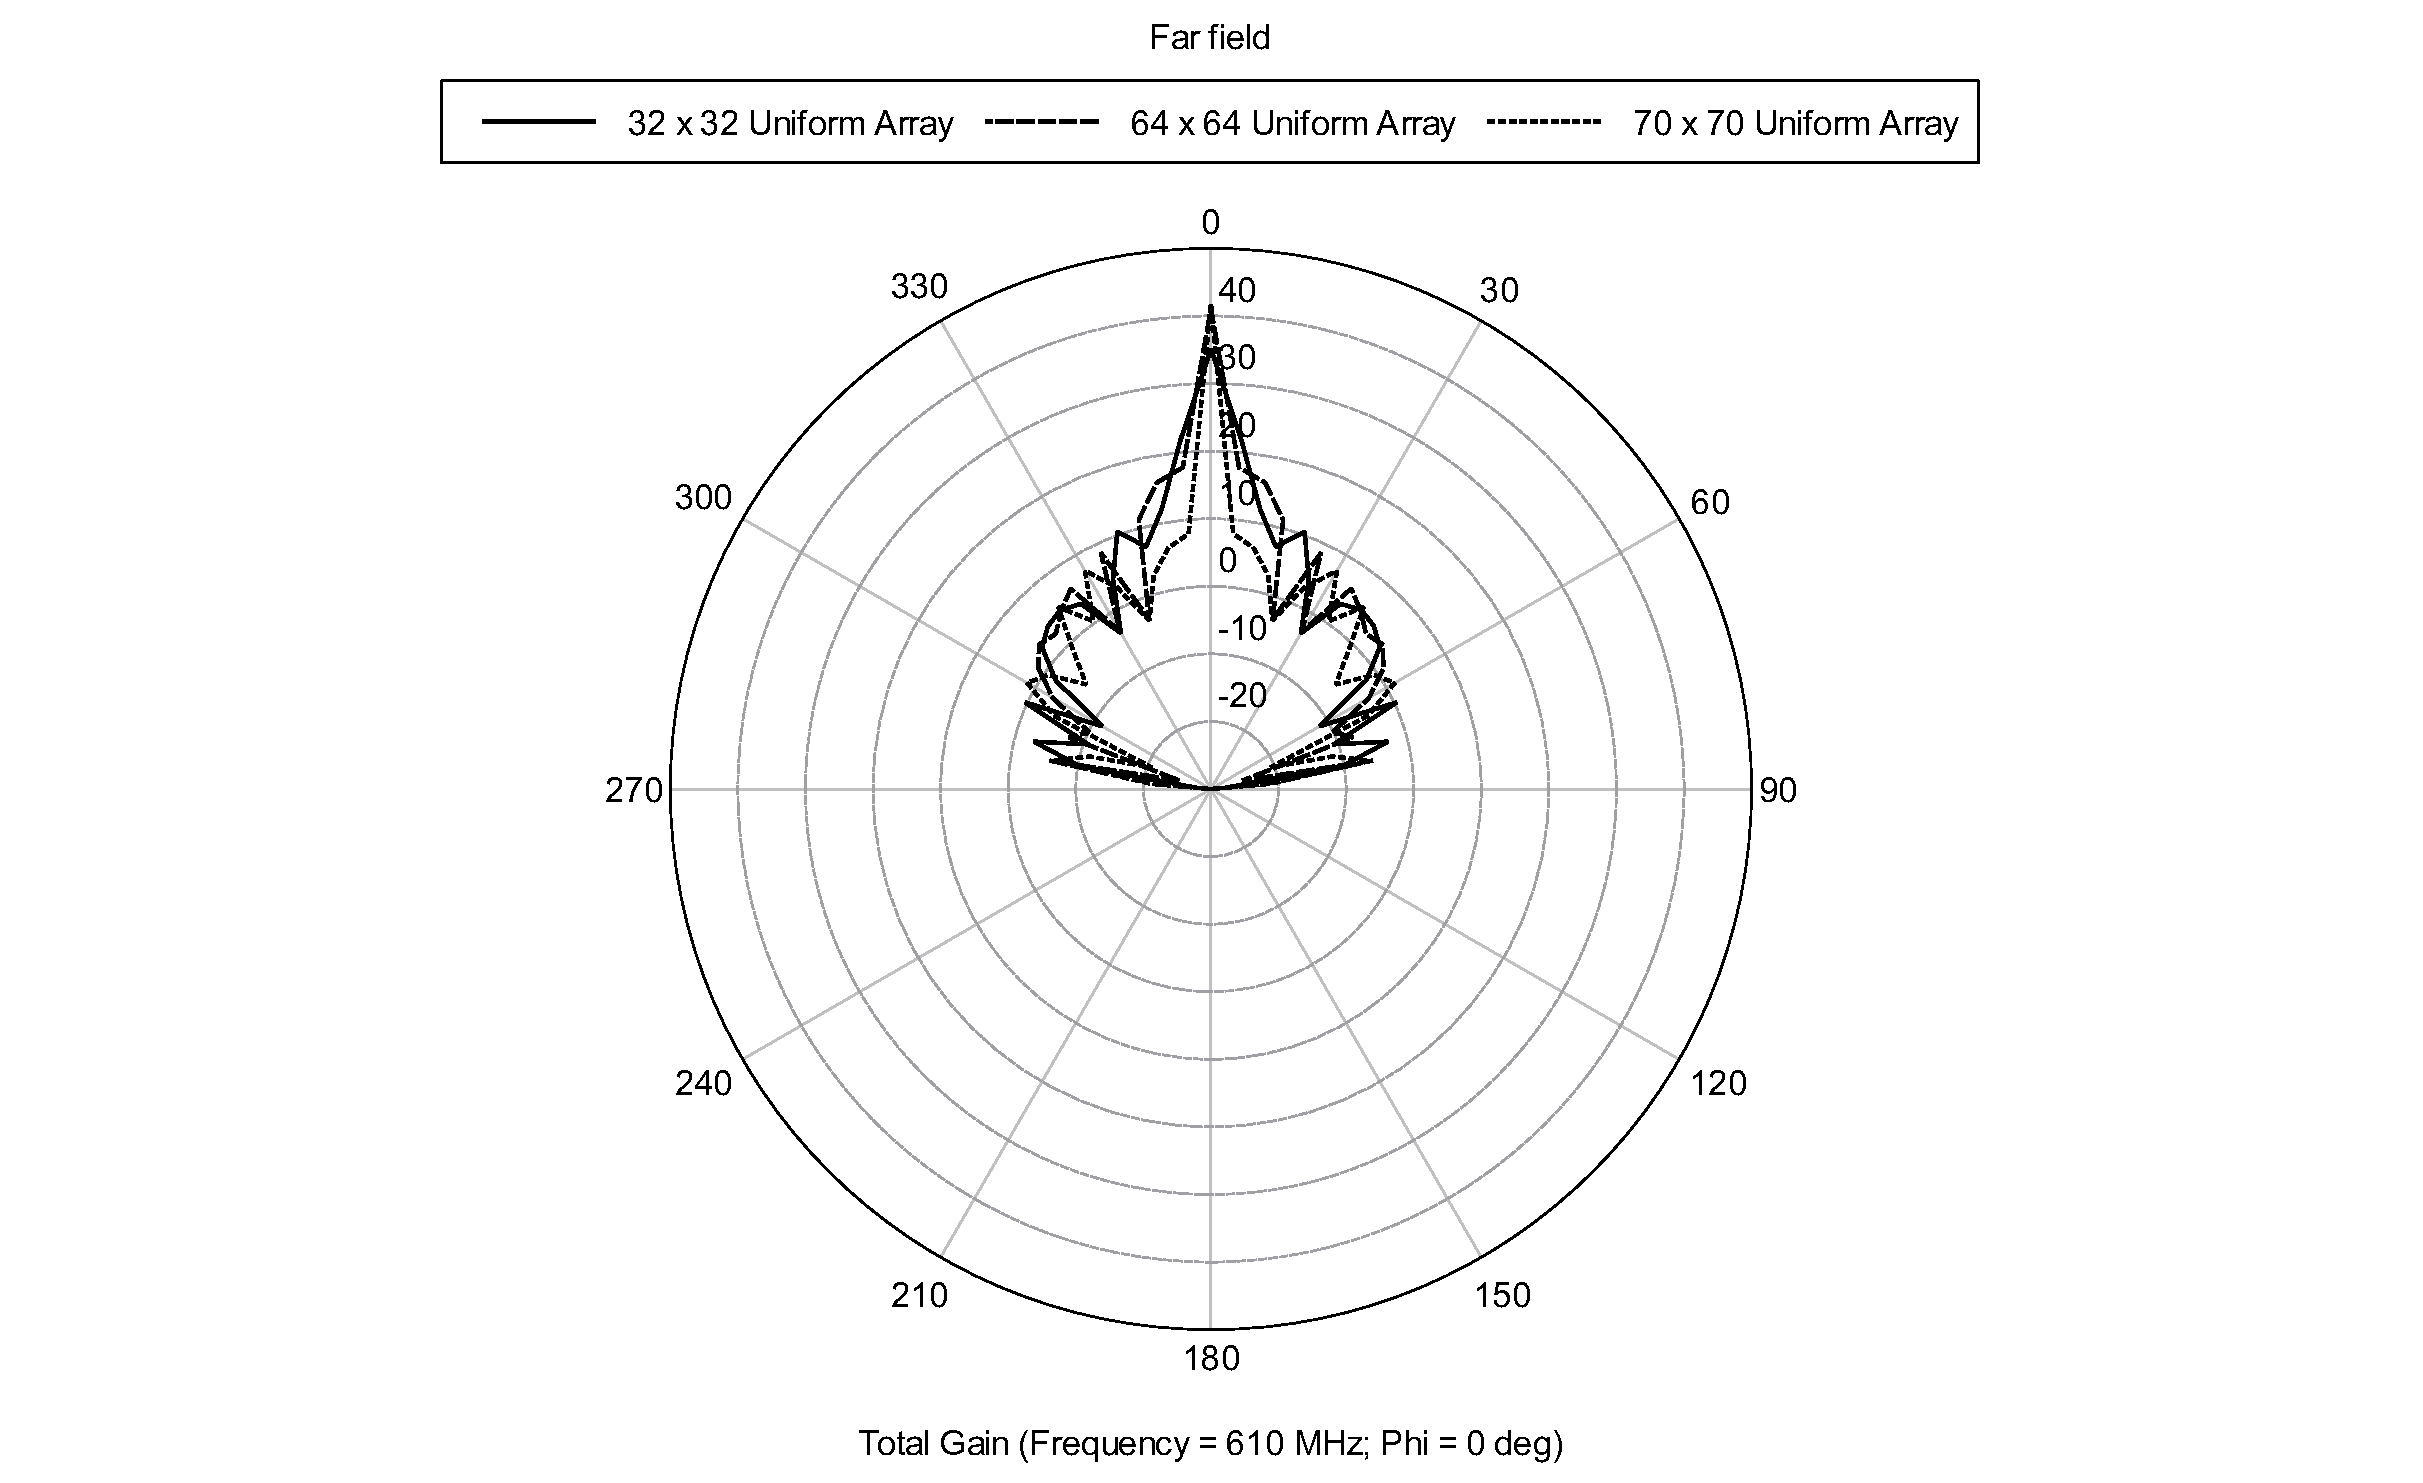
\includegraphics[width=0.9\linewidth]{BigArrayGain-Polar.pdf}
            \caption{Main Beam Gain for Different Array Sizes - Polar Plot}
            \label{fig:MainBeamGain-Polar}
        \end{subfigure}%
        \begin{subfigure}{.5\textwidth}
            \centering
            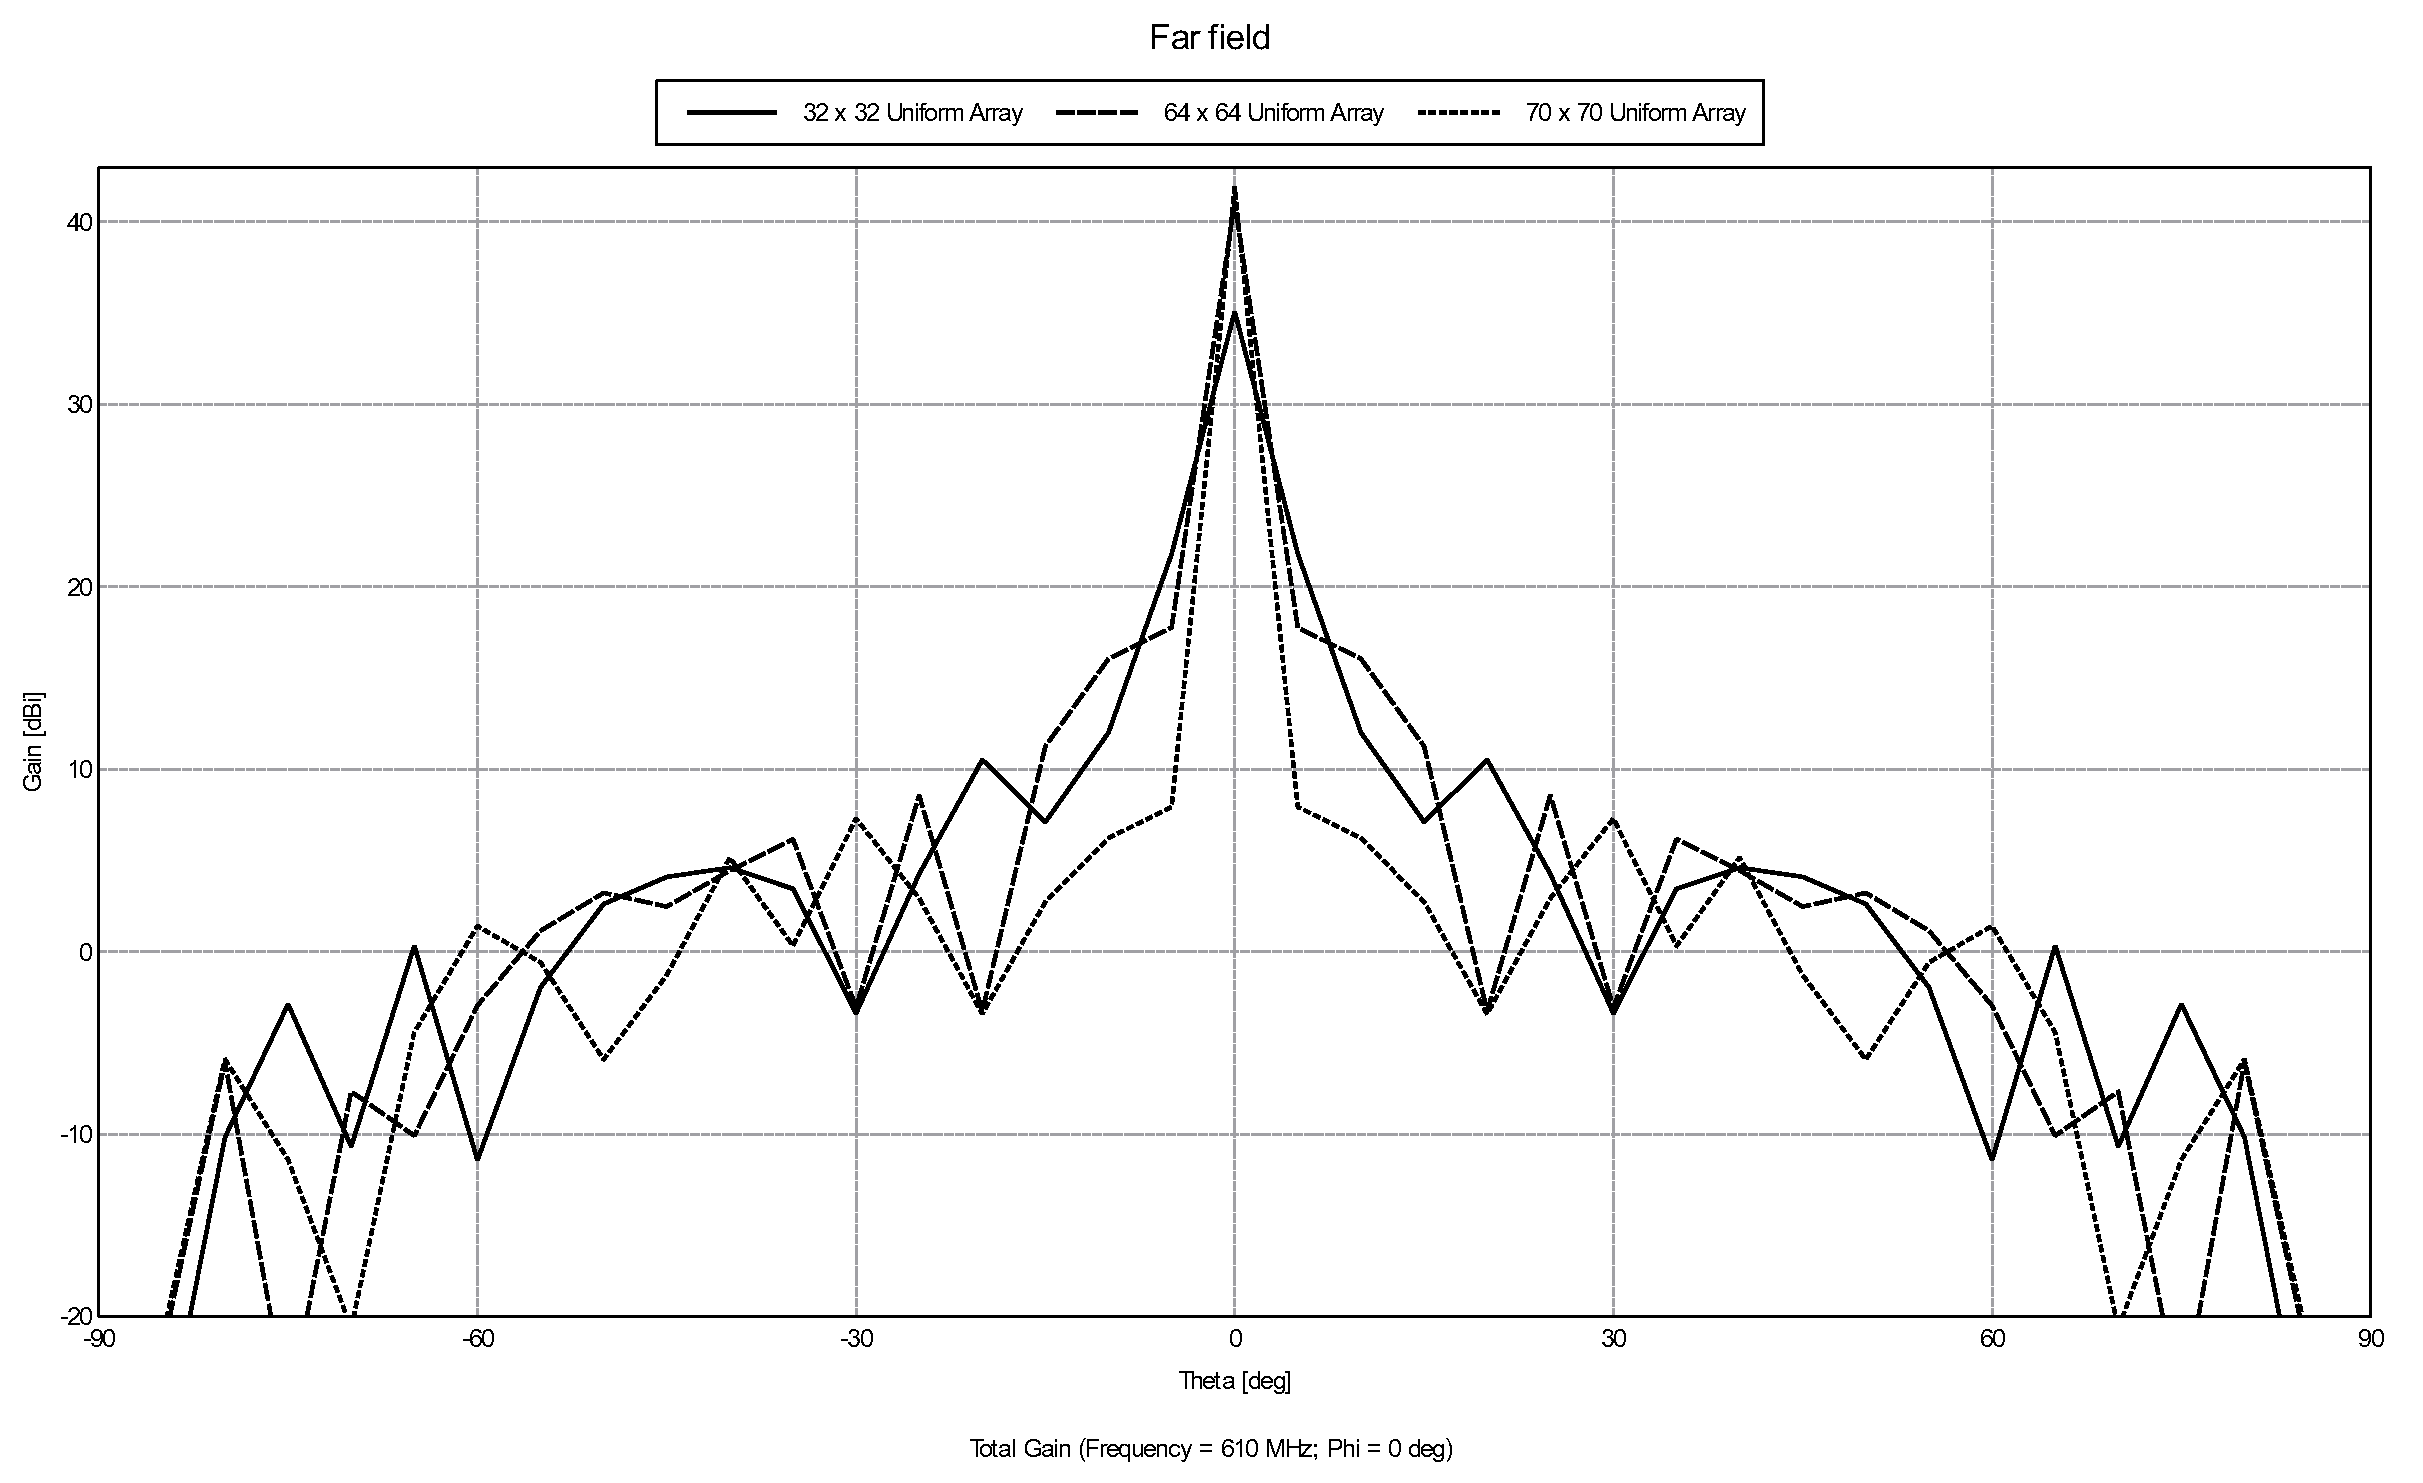
\includegraphics[width=0.9\linewidth]{BigArrayGain-Cartesian.pdf}
            \caption{Main Beam Gain for Different Array Sizes - Cartesian Plot}
                \label{fig:MainBeamGain-Cartesian}
            \end{subfigure}
\caption{Main Beam Gain for Different Array Sizes}
\label{fig:MainBeamGain}
\end{figure}




The drawback of increasing the number of elements in the array (even though the main beam gain has increased), is that the side lobe level decreases. This implies that these side lobes may be capable of creating false detections. If the side lobe levels are high enough, they may be capable of sending out an EM wave with enough energy such that the returned pulse is detected as an object. Depending on the direction of these side lobes, it may be low flying aircraft, birds, objects in the low range of LEO, etc. Consequently, these side lobes should be reduced such that they do not affect the system.
Side lobes can create unwanted interference between neighbouring systems which is disadvantageous for both systems. In the case that the beam is steered in its maximum angle, this side lobe is steered as well. 
A number of methods exist in which to reduce this effect, the first is to attempt to reduce the side lobes.
The reduction of these side lobes is discussed further in section~\ref{sec:ElementExcitation}.

In this section, it is pertinent to note the difference between the use of a ground plane and the absence of a ground plane, Fig.~\ref{fig:GroundPlane} illustrates this difference in the case of a $32 \times 32$ antenna array.


\begin{figure}[htb]
    \centering
    \begin{subfigure}{.5\textwidth}
        \centering
            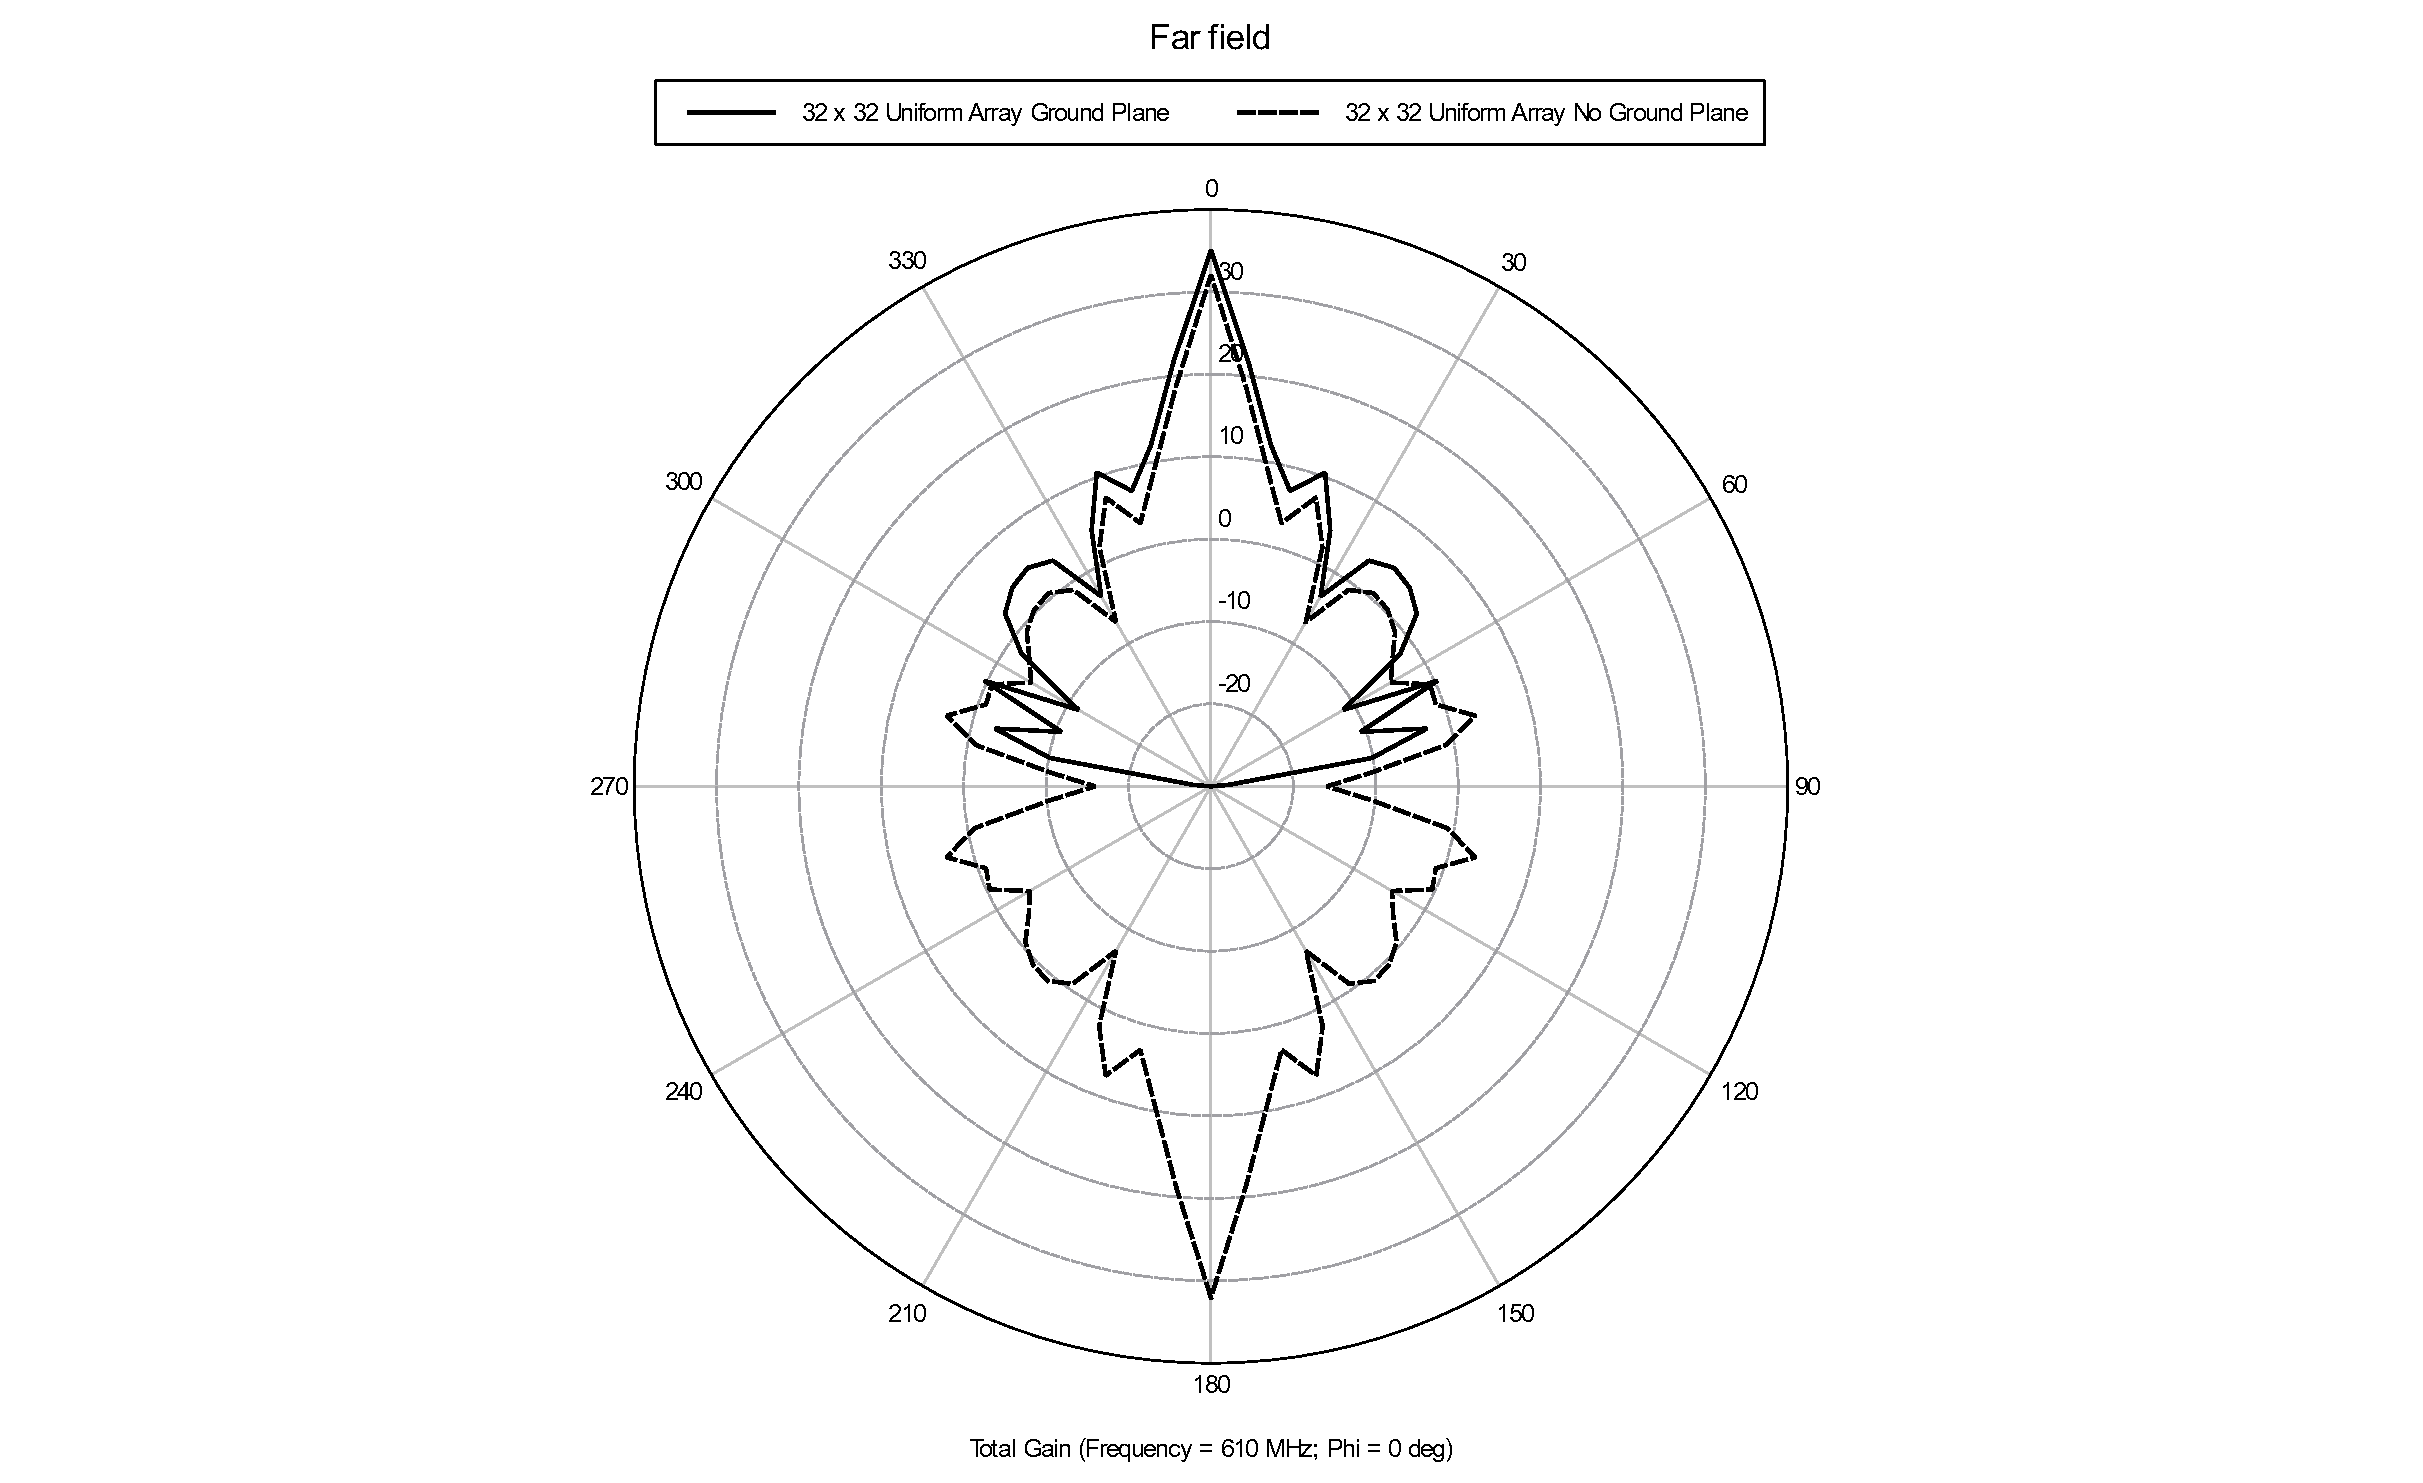
\includegraphics[width=0.9\linewidth]{GroundPlane-Polar.pdf}
            \caption{Ground Plane vs No Ground Plane - Polar Plot}
            \label{fig:GroundPlane-Polar}
        \end{subfigure}%
        \begin{subfigure}{.5\textwidth}
            \centering
            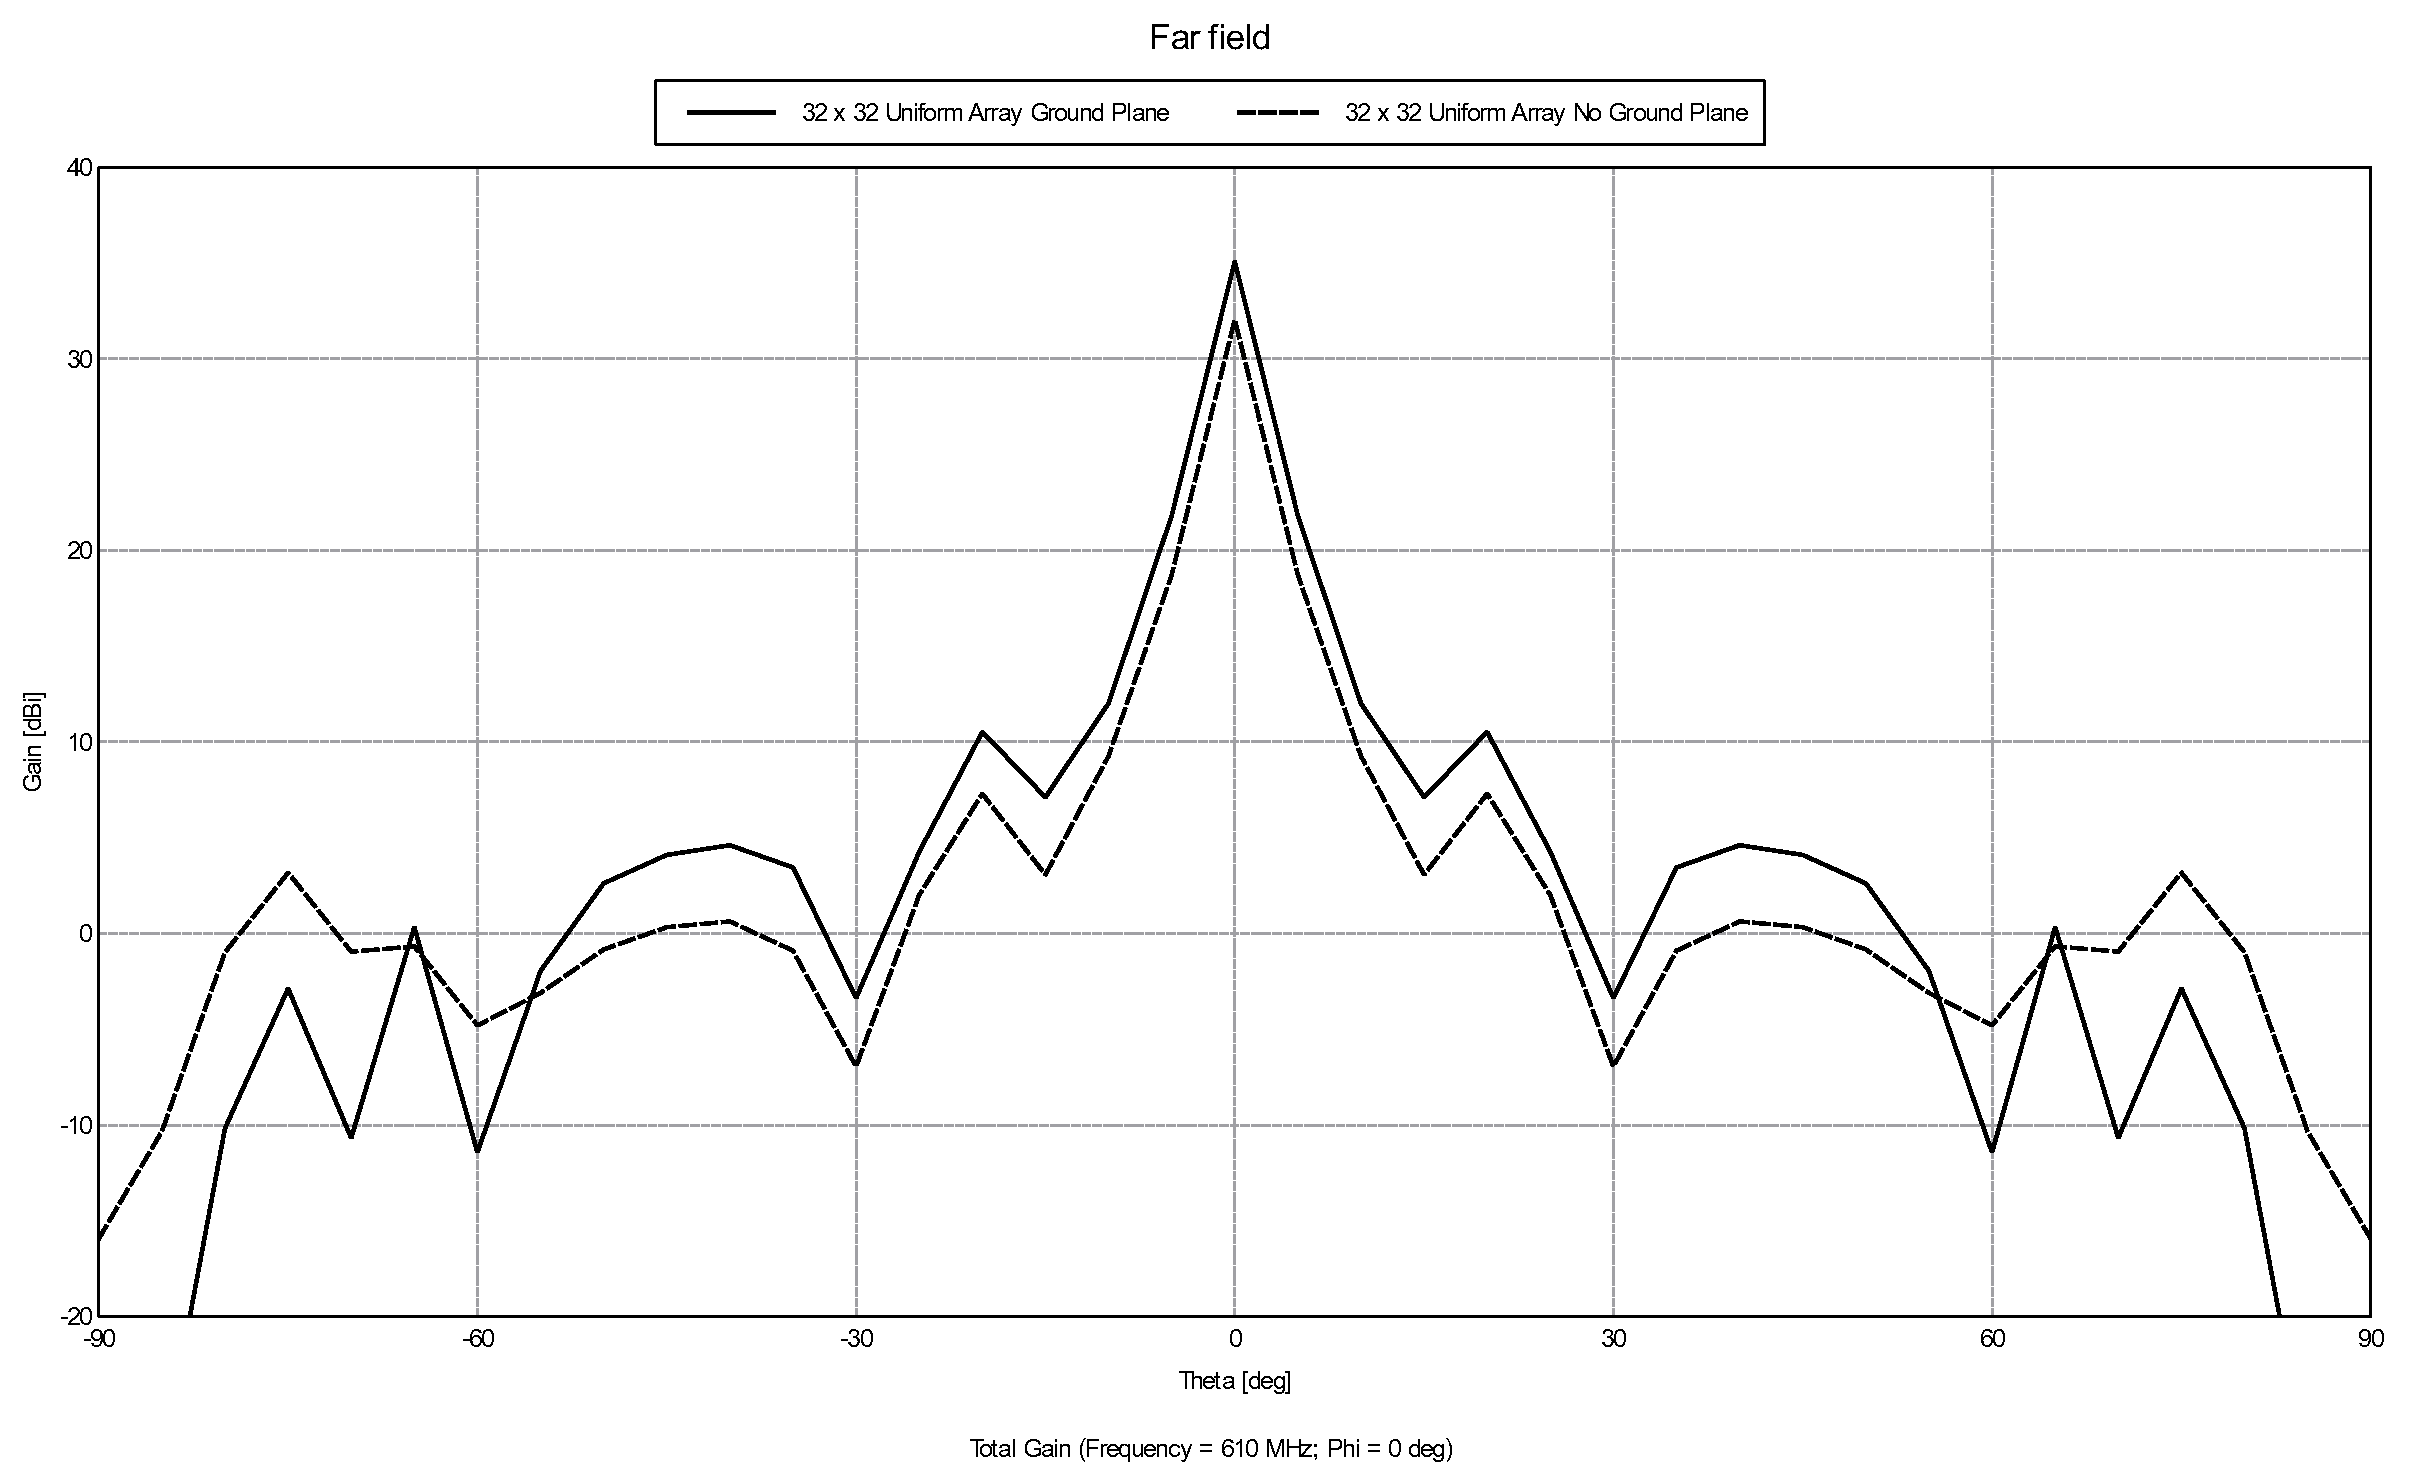
\includegraphics[width=0.9\linewidth]{GroundPlane-Cartesian.pdf}
            \caption{Ground Plane vs No Ground Plane - Cartesian Plot}
                \label{fig:GroundPlane-Cartesian}
            \end{subfigure}
\caption{Ground Plane vs No Ground Plane}
\label{fig:GroundPlane}
\end{figure}

Fig.~\ref{fig:MainBeamGain} and \ref{fig:GroundPlane} illustrate the different gains acquirable based on the sizing of the array and how the ground plane affects the system.
Table~\ref{tab:AmplitudeTapering} lists the important parameters from the three different arrays in Fig.~\ref{fig:MainBeamGain} as these parameters are pertinent to the functioning of the system.


\subsection{Element Phasing} \label{sec:ElementPhasing}
In order to achieve steering of the array, progressive phase delay is required for each element. This phase delay amount is determined with the use of equation~\ref{eqn:PhaseDelay} \cite[p.~301]{Balanis}.

\begin{equation} \label{eqn:PhaseDelay}
\Psi = k d cos \theta + \beta
\end{equation}
In this case $\Psi$ represents the angle to which the array should direct its main lobe, $\theta$ is taken to be $0^{\circ}$ (to create the broadside effect) and $\beta$ the progressive phase delay for each element.
This principle is used to illustrate the scanning feature represented in Fig.~\ref{fig:SteeringSmall} where different scanning angles are illustrated by the differing curves. This scenario makes use of a $32 \times 32$ array where the steering is increased by $10^{\circ}$ increments.

This principle can be applied continuously which means that the beam can be dynamically steered in the required direction.
% The change in direction that the beam is steered is dependent on the external 
In order to apply this principle to the 2D array used in this design, the steering is implemented in the $x$ direction, and then the $y$ direction, such that the beam is steered in the $\theta$ and then the $\phi$ direction in order to be directed at the required coordinates.
This system is analysed with the use of FEKO in order to test the steering ability of the system \cite{FEKO}. The Python code used to generate the phasing can be found in section *** python code.


\begin{figure}[htb]
    \centering
    \begin{subfigure}{.5\textwidth}
        \centering
            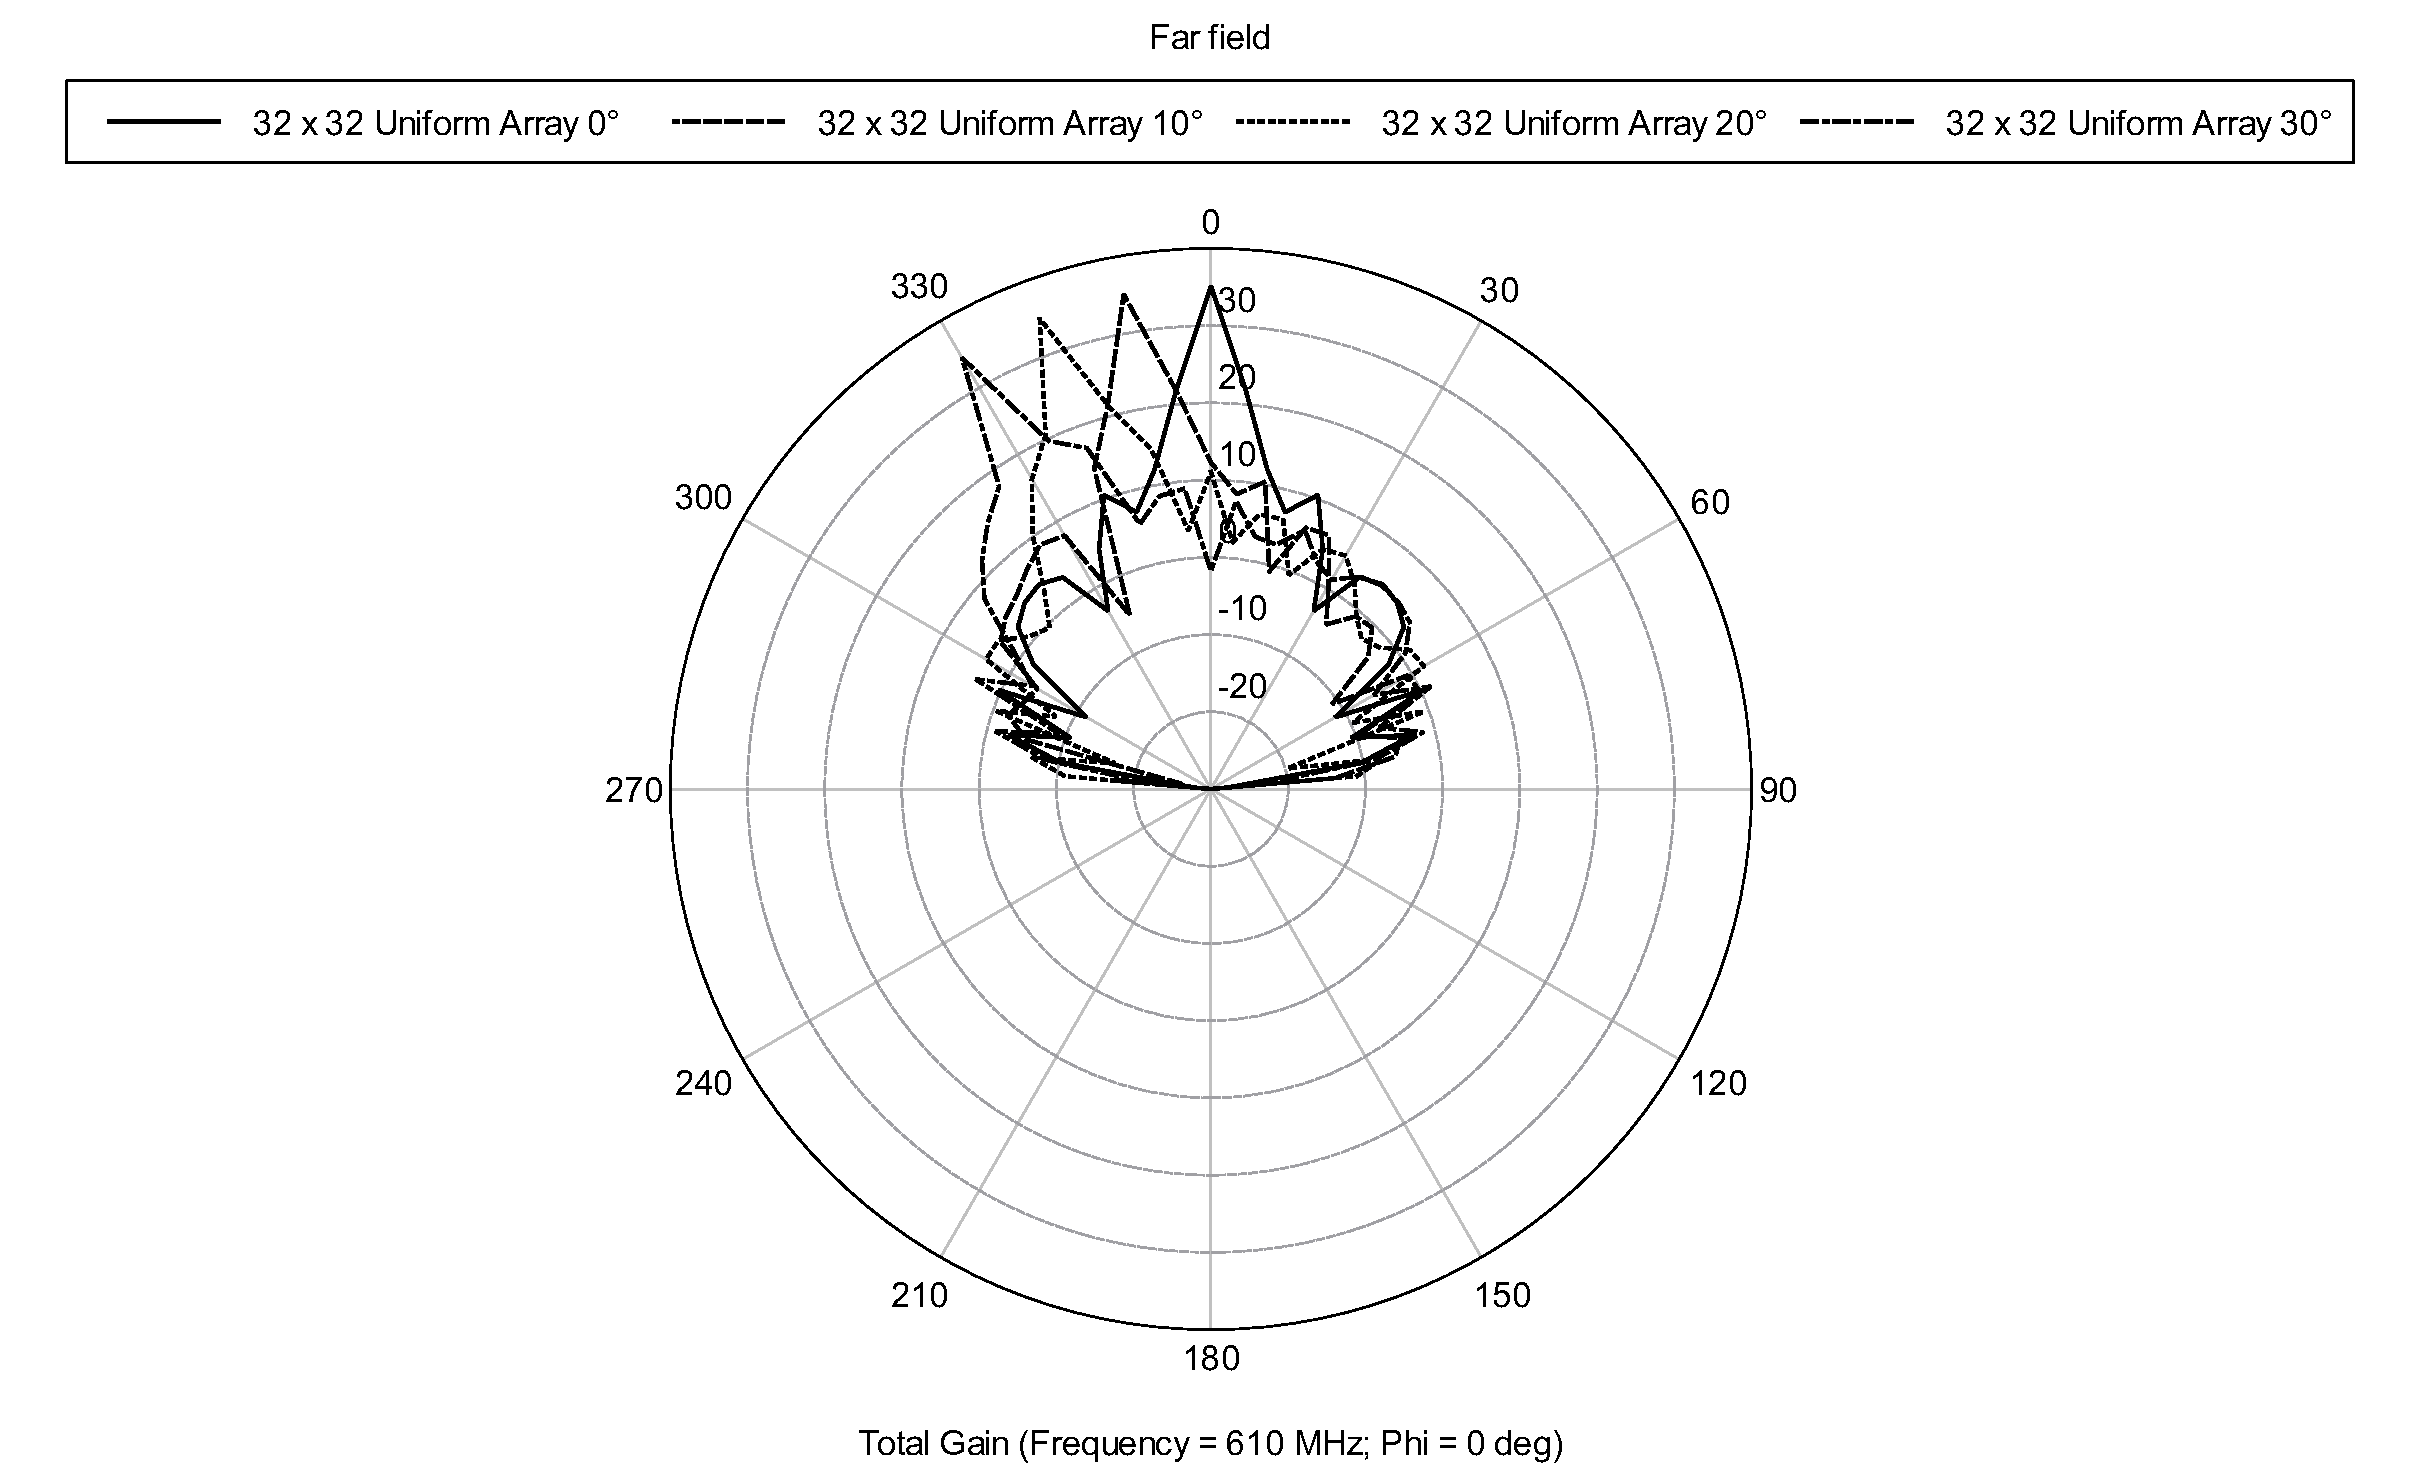
\includegraphics[width=0.9\linewidth]{SteeringSmall-Polar.pdf}
            \caption{$32 \times 32$ Array Beam Steering Ability - Polar Plot}
            \label{fig:SteeringSmall-Polar}
        \end{subfigure}%
        \begin{subfigure}{.5\textwidth}
            \centering
            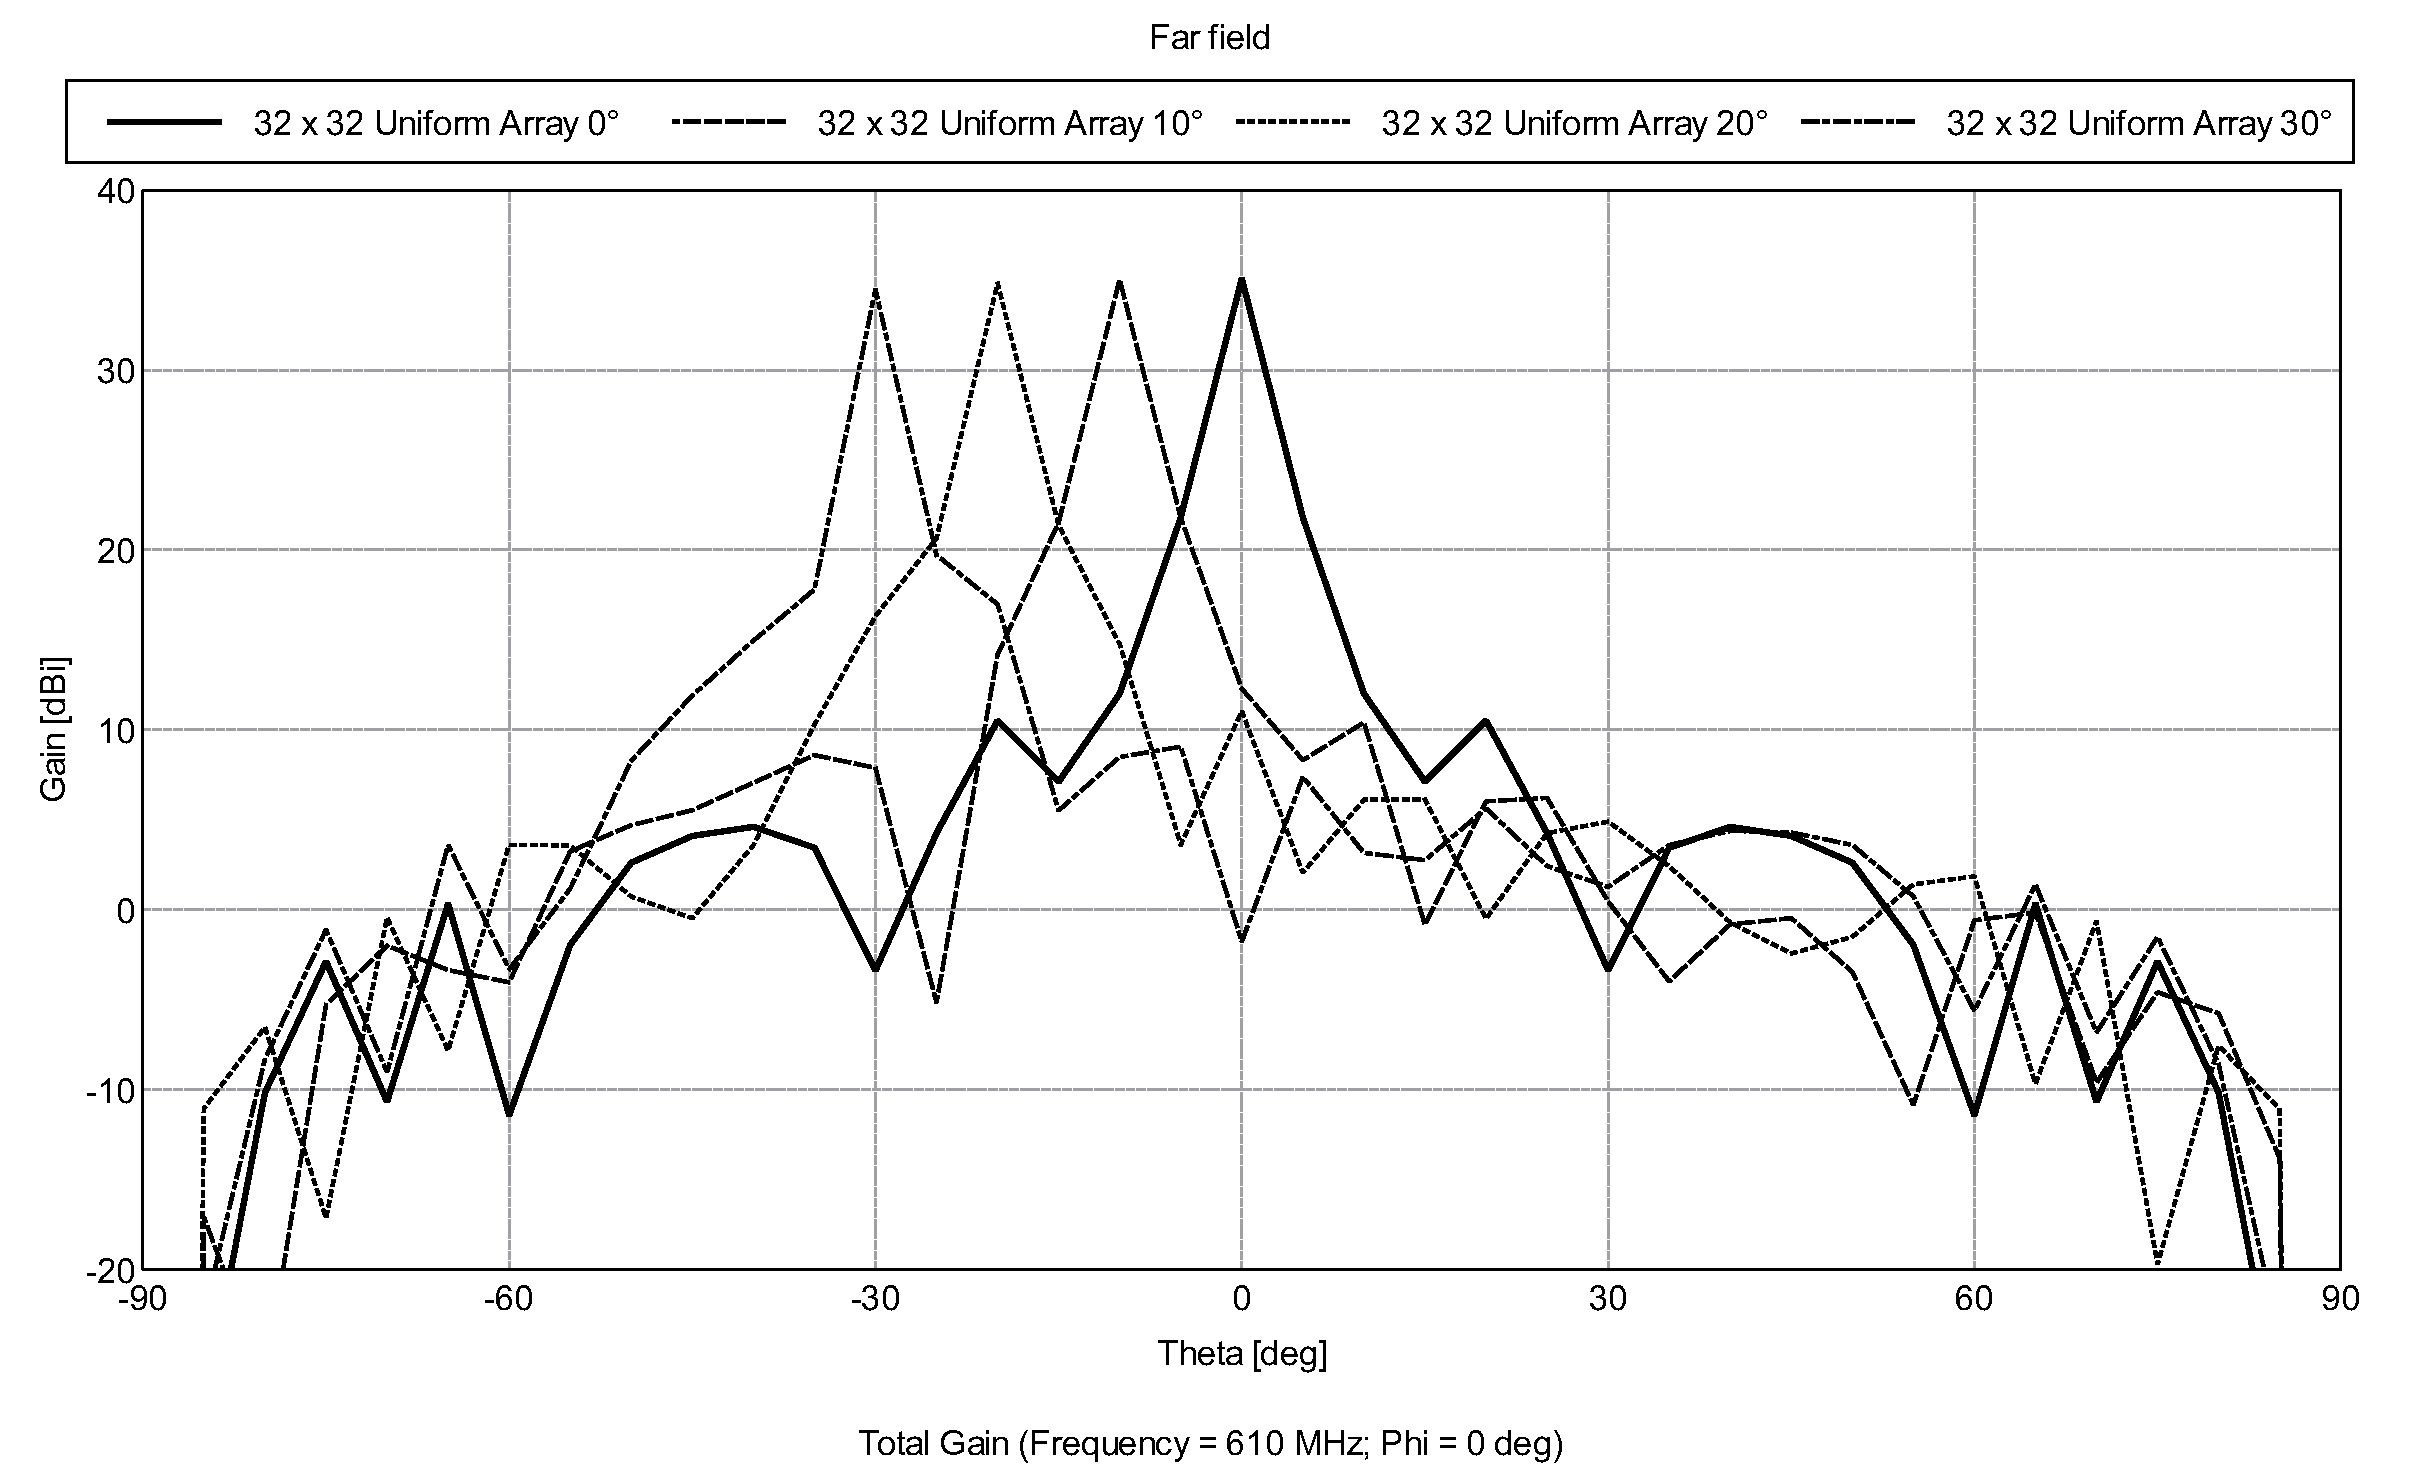
\includegraphics[width=0.9\linewidth]{SteeringSmall-Cartesian.pdf}
            \caption{$32 \times 32$ Array Beam Steering Ability- Cartesian Plot}
                \label{fig:SteeringSmall-Cartesian}
            \end{subfigure}
\caption{$32 \times 32$ Array Beam Steering Ability}
\label{fig:SteeringSmall}
\end{figure}


Following the steering ability of a smaller array in Fig.~\ref{fig:SteeringSmall}, it is scaled up to the full sized array, in this case, the curves represent a $0^{\circ}$, $10^{\circ}$, and a $20^{\circ}$ shift this is illustrated in Fig.~ref{fig:SteeringBig}.

\begin{figure}[htb]
    \centering
    \begin{subfigure}{.5\textwidth}
        \centering
            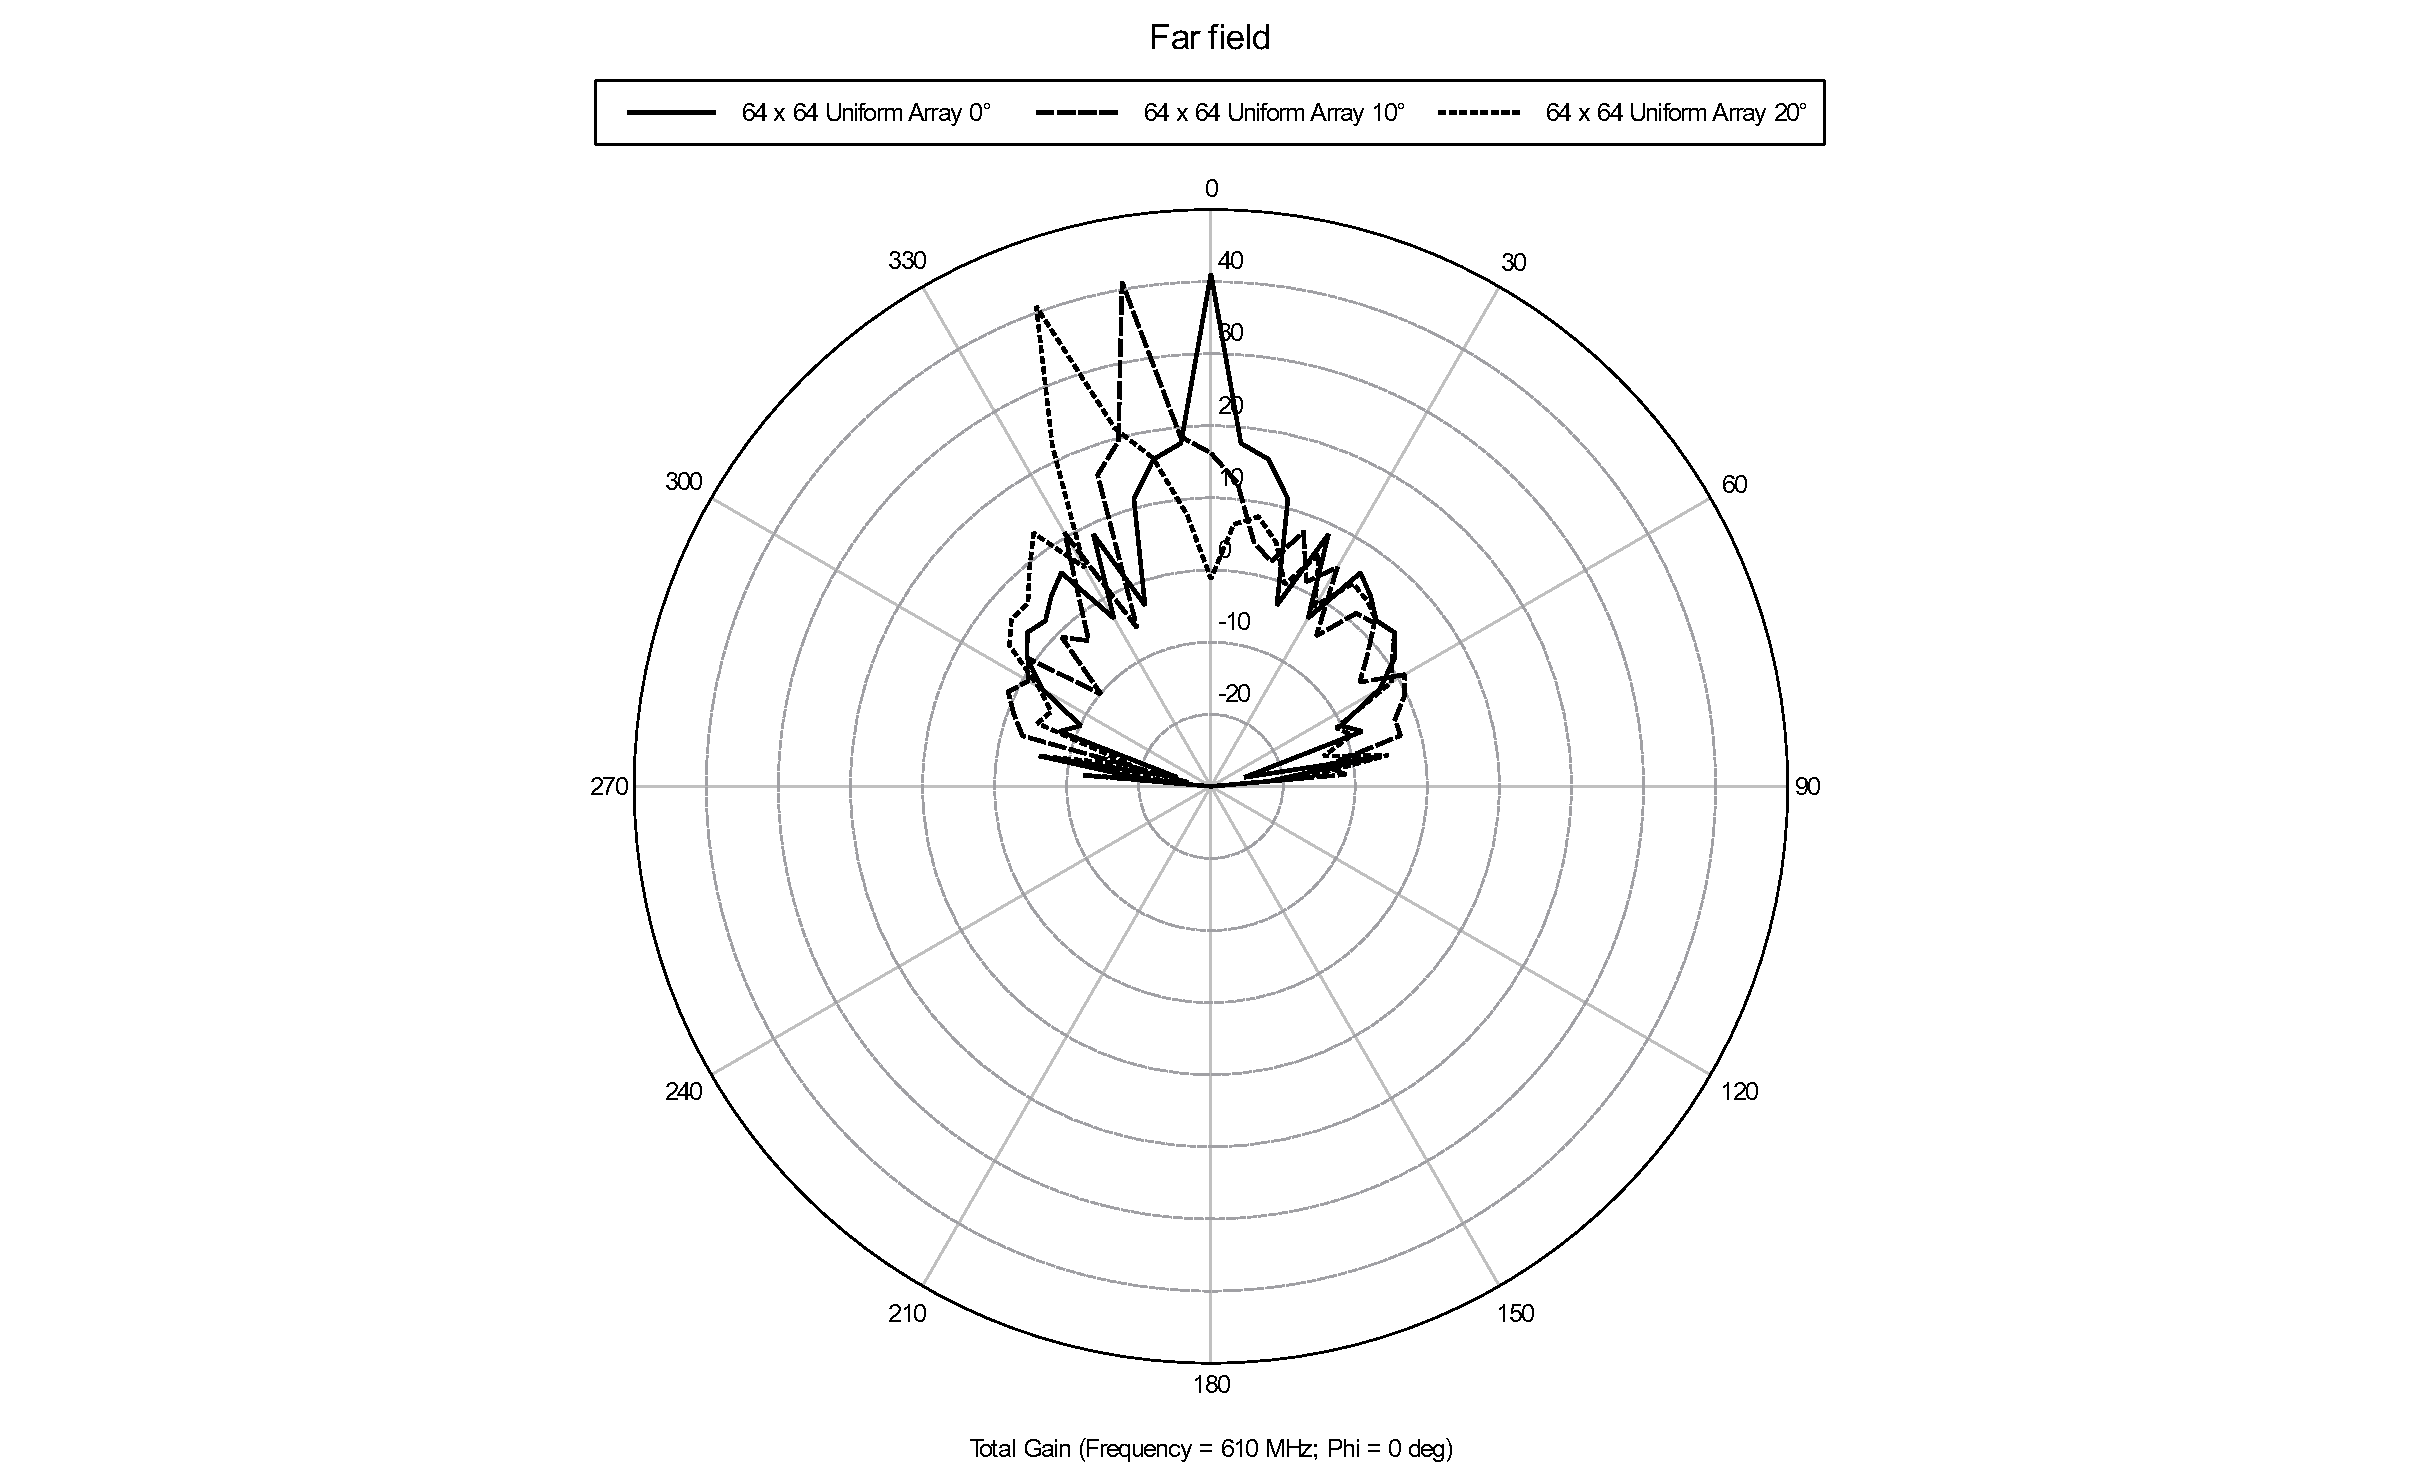
\includegraphics[width=0.9\linewidth]{SteeringBig-Polar.pdf}
            \caption{$64 \times 64$ Array Beam Steering Ability - Polar Plot}
            \label{fig:SteeringBig-Polar}
        \end{subfigure}%
        \begin{subfigure}{.5\textwidth}
            \centering
            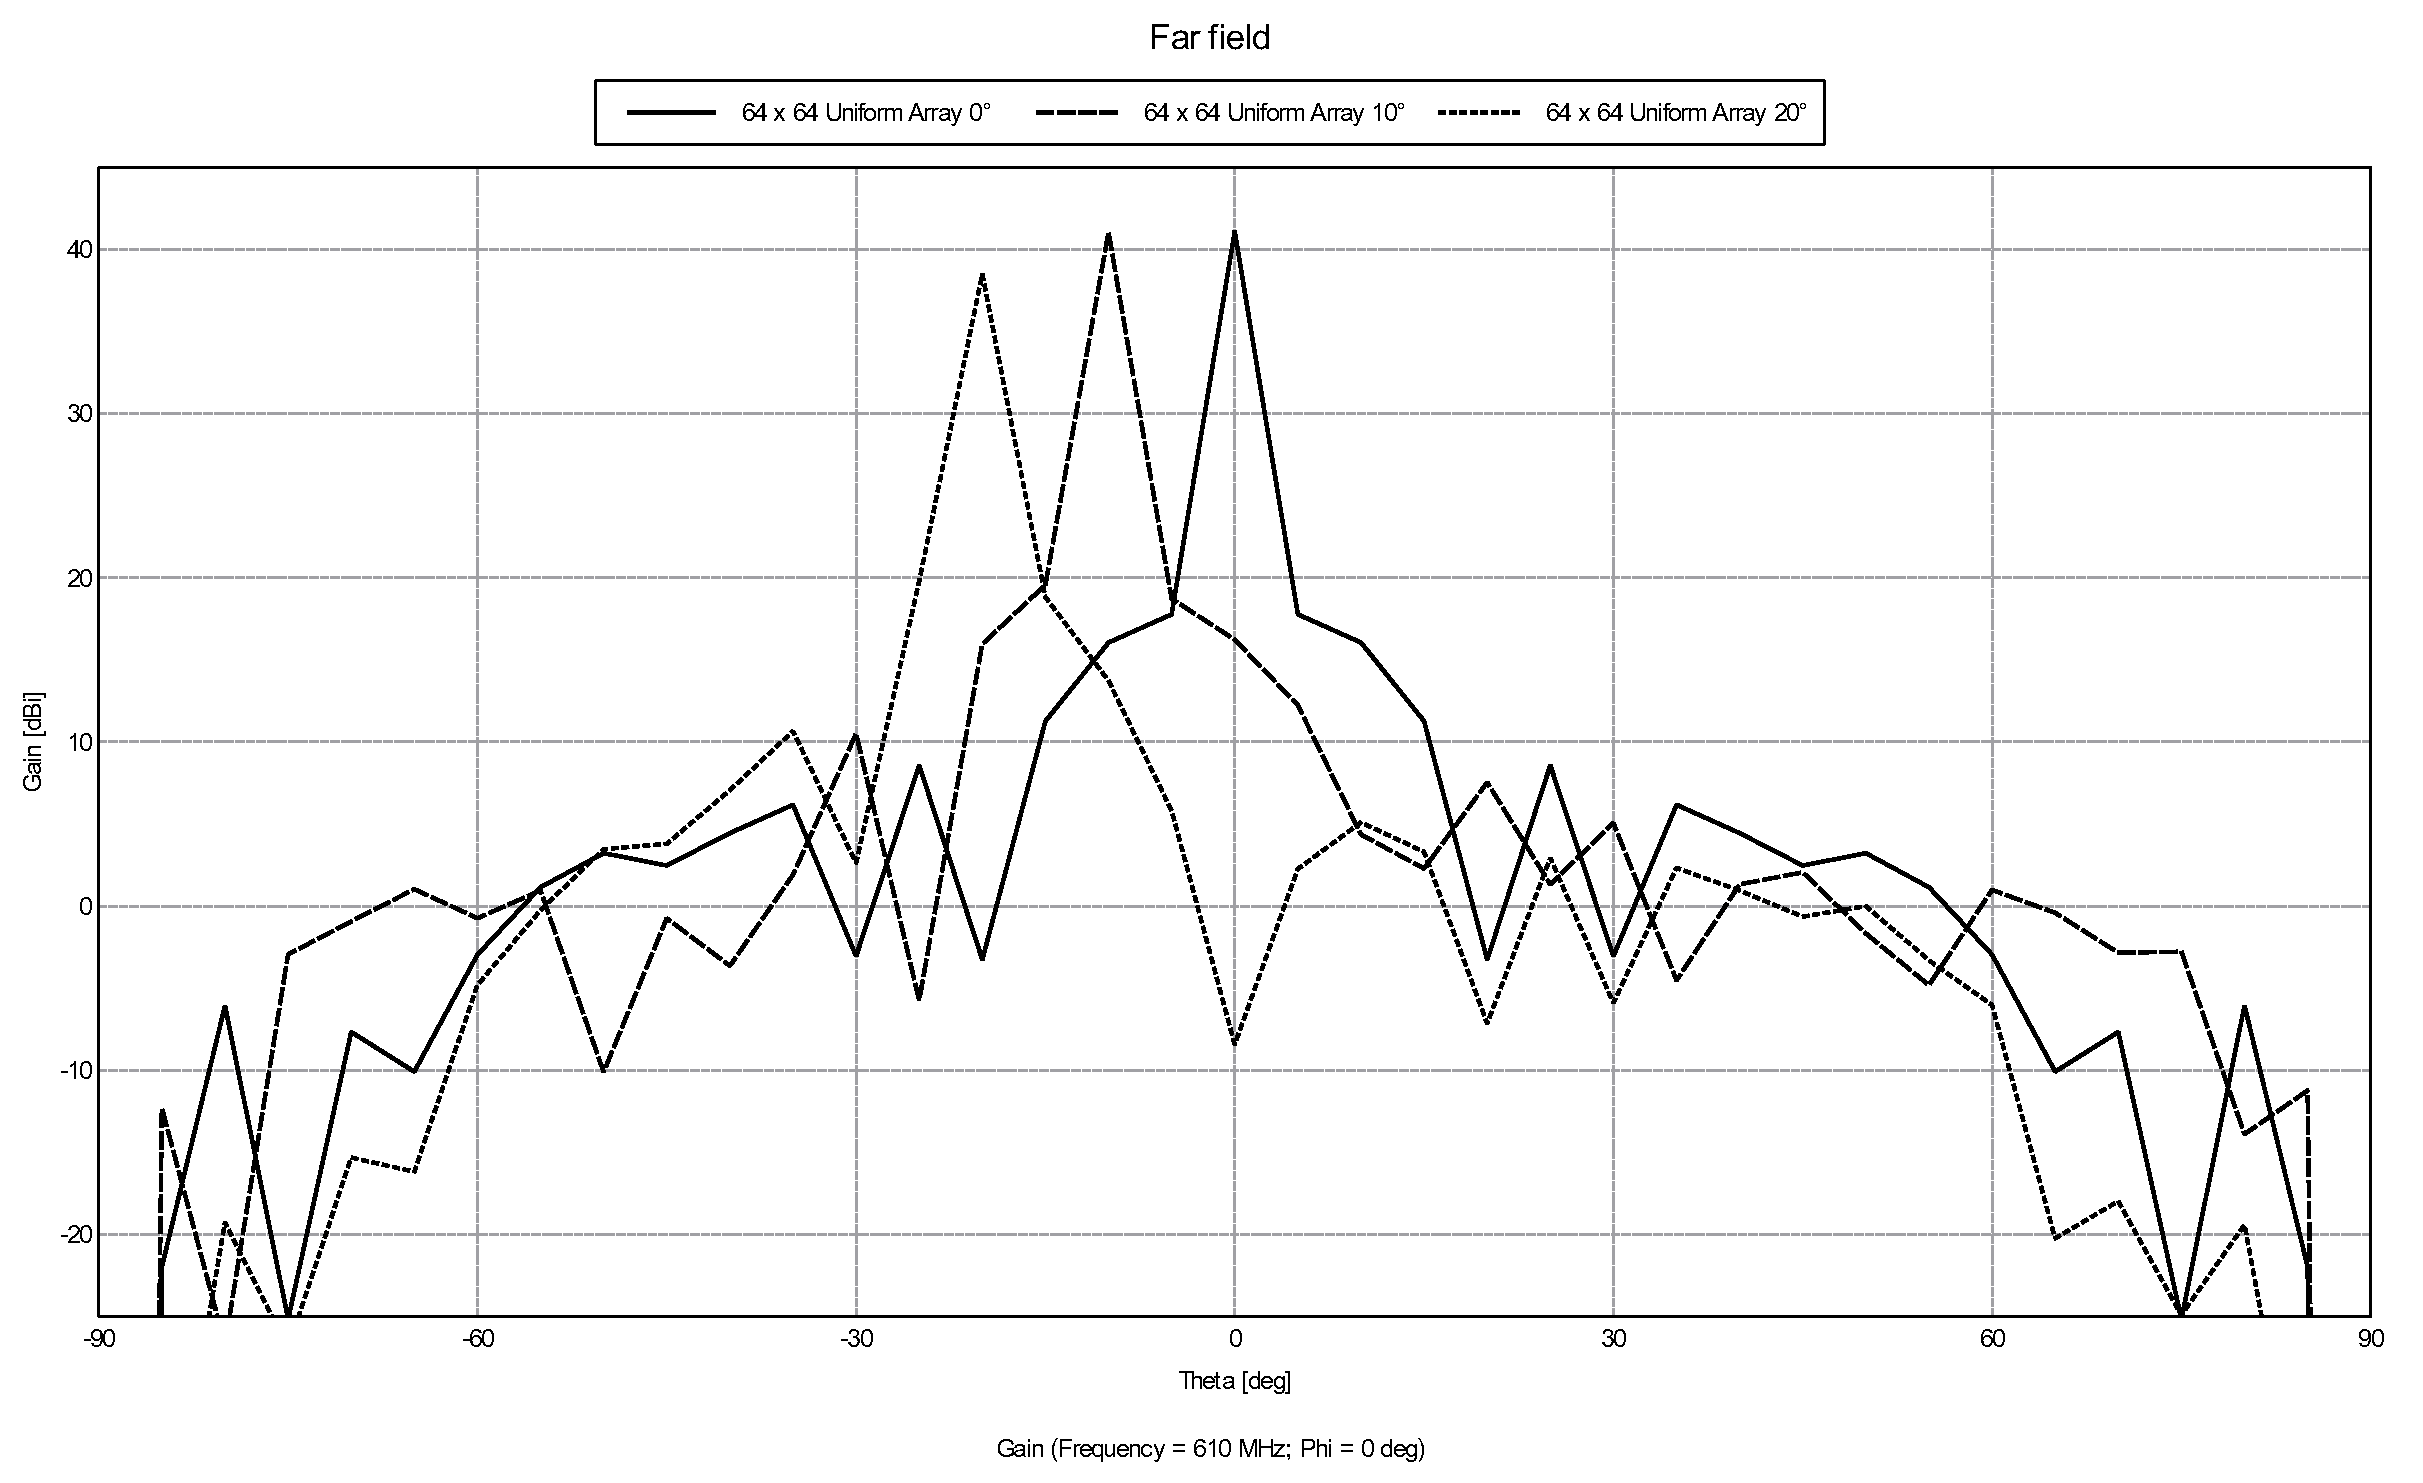
\includegraphics[width=0.9\linewidth]{SteeringBig-Cartesian.pdf}
            \caption{$64 \times 64$ Array Beam Steering Ability- Cartesian Plot}
                \label{fig:SteeringBig-Cartesian}
            \end{subfigure}
\caption{$64 \times 64$ Array Beam Steering Ability}
\label{fig:SteeringBig}
\end{figure}


The introduction of more antenna elements results in a decreasing main lobe width, this is wanted as it reduces the cross-range resolution when detecting objects\cite[p.~14,28,469]{radarHandbook}.
The phasing is achieved with the feeding network which is designed in section~\ref{sec:FeedingNetworks}.

\subsection{Element Excitation} \label{sec:ElementExcitation}
Side lobe level of an array is always present in cases where a uniform excitation of the array is used. These side lobes can become dangerous when the size and power level of the array becomes large.
There are a number of ways in which to reduce the side lobes: Uniform, Binomial, and Tschebyscheff \cite[p.~324-325]{Balanis}. Uniform is the standard case which has been used up to this point, and the Tschebyscheff is not implemented in this system. The uniform distribution does not attempt to reduce the side lobes, however, it is simple to implement in many situations as this reduces the cost and complexity of the system.
The second makes use of the Binomial distribution in order to weight the power which excites each antenna element.
This method however, implies that in the case that the array becomes large, the outside elements contribute minuscule amounts of power to the system.
Consequently, a compromise between the binomial and the uniform amplitude is created.
This is done such that, the power is tapered from the center of the array, and the power is tapered down to a set point at the edges of the array. This tapering is set to be a $50 \%$ value such that the middle elements transmit $100~\%$ of the power, and the outside transmit $50~\%$ of the power. This results in a pyramidal distribution on the array as it tapers off to the edges.
This power taper in the elements is illustrated in Fig.~\ref{fig:PowerTaperingHeatMap} where the darker colour represents a higher power.

\begin{figure}[htb]
    \centering
    \begin{subfigure}{.5\textwidth}
        \centering
            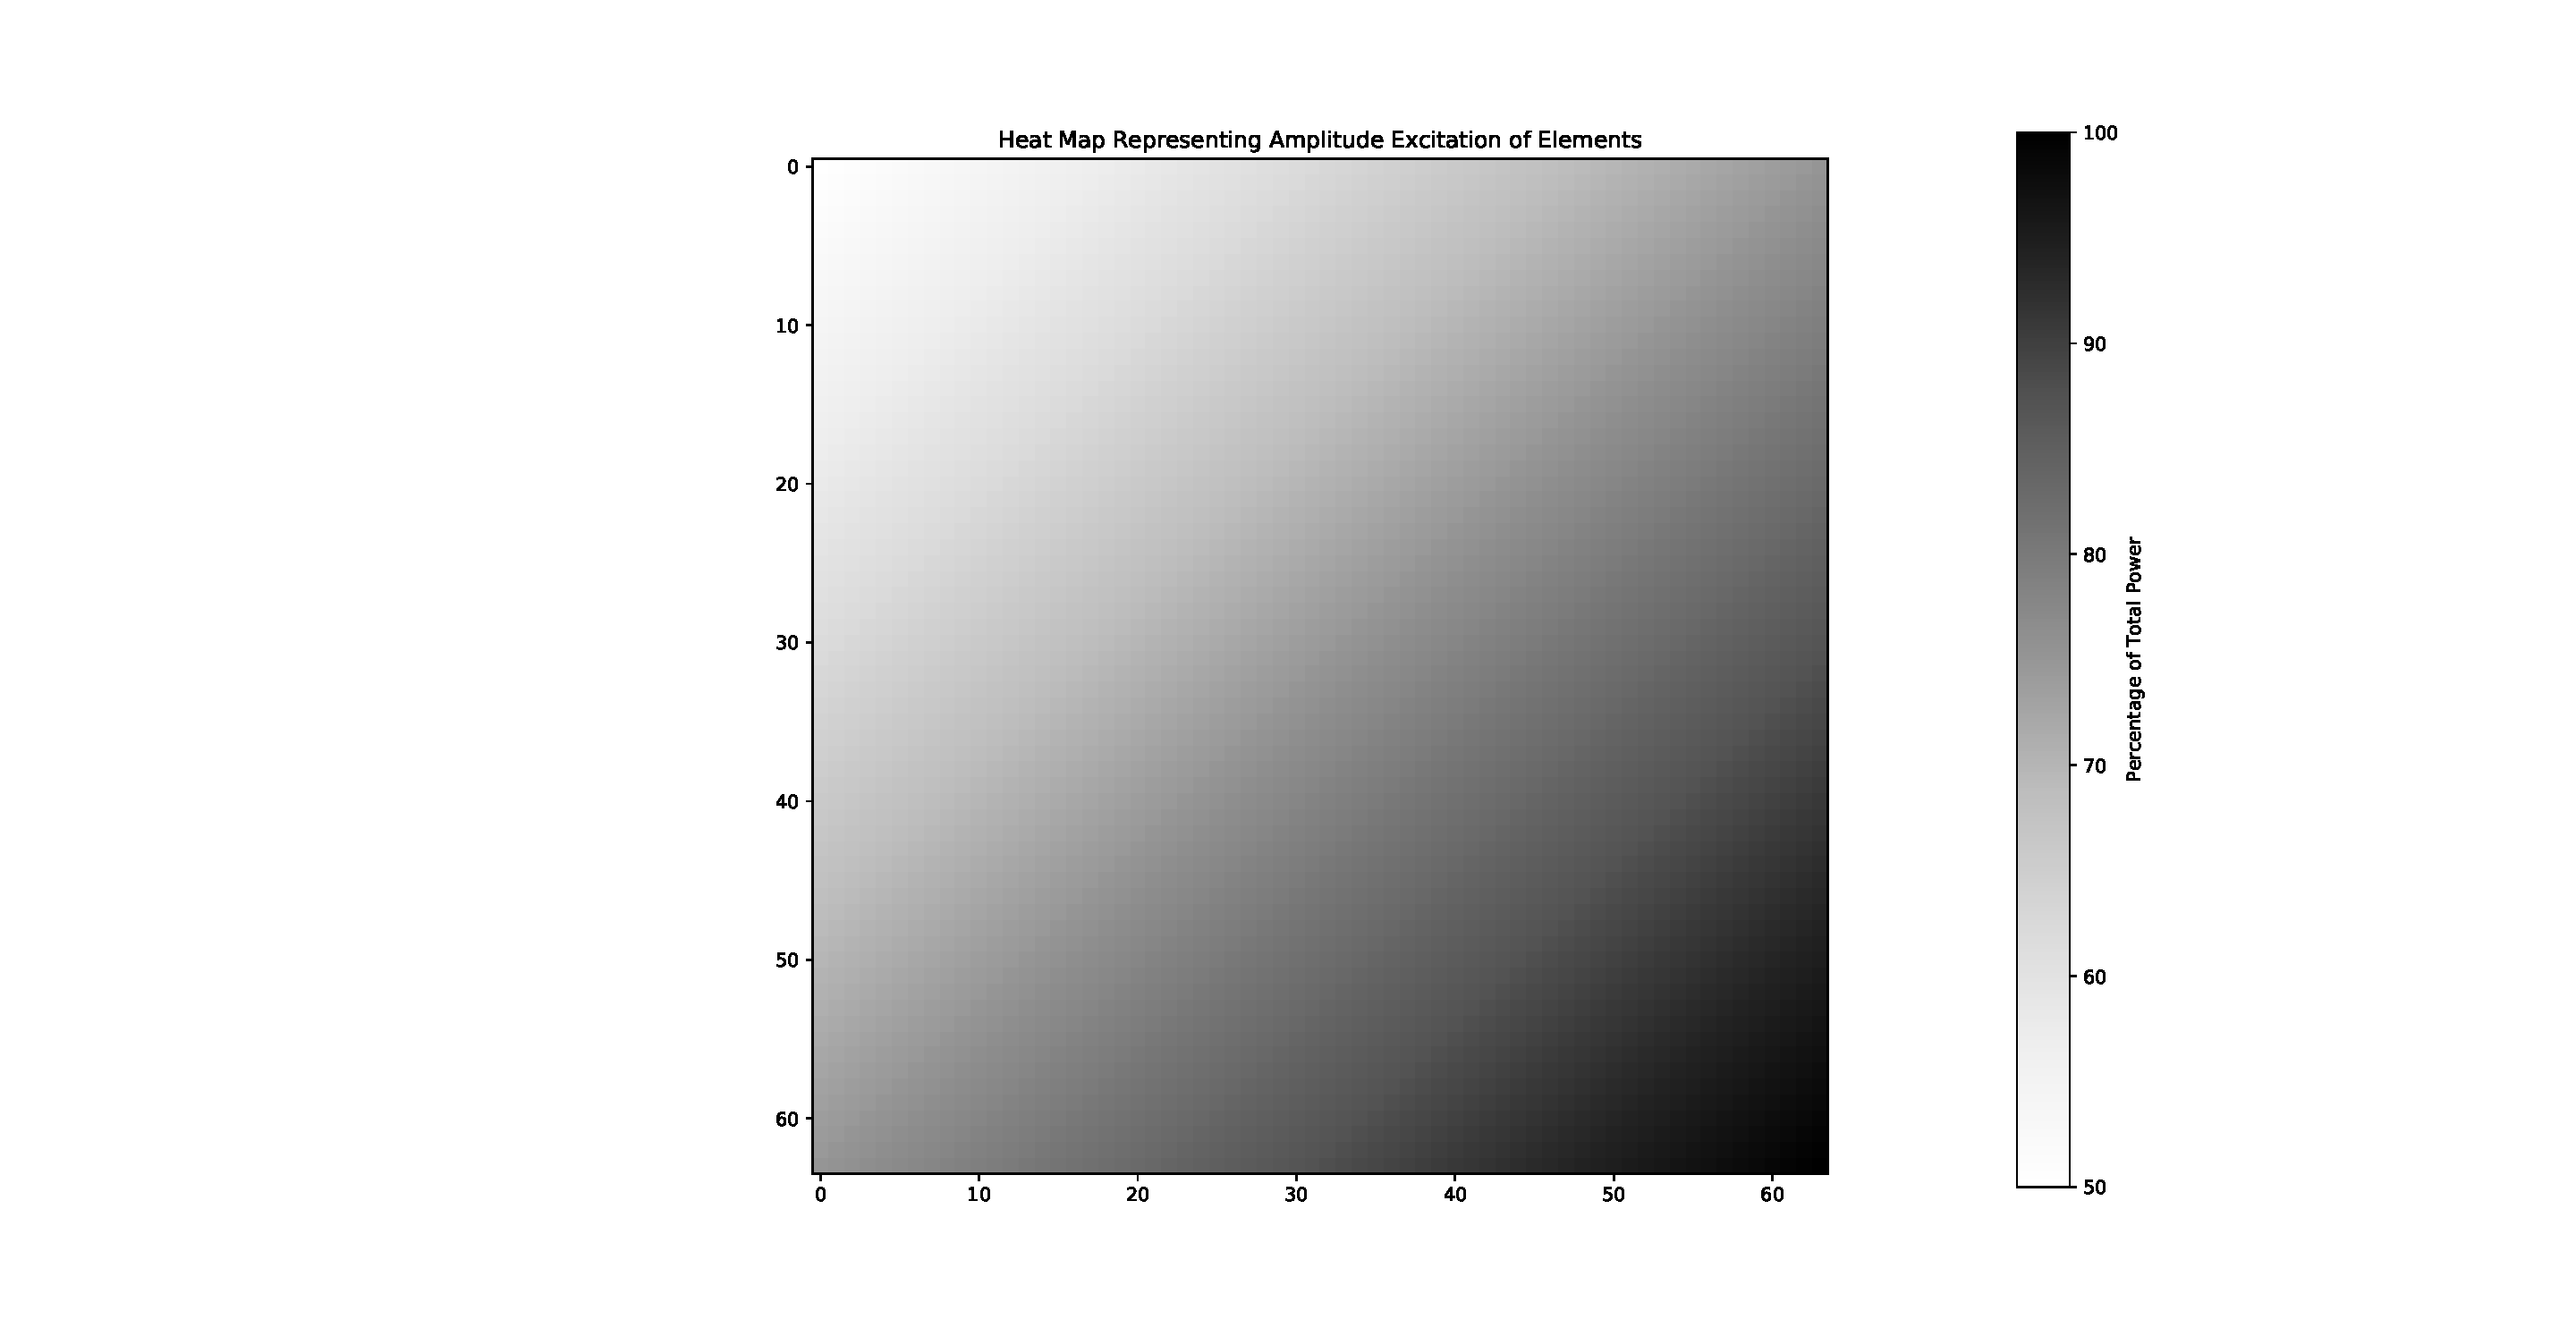
\includegraphics[width=0.9\linewidth]{PowerTapering.pdf}
            \caption{Power Tapering}
            \label{fig:PowerTaperingHeatMap}
        \end{subfigure}%
        \begin{subfigure}{.5\textwidth}
            \centering
            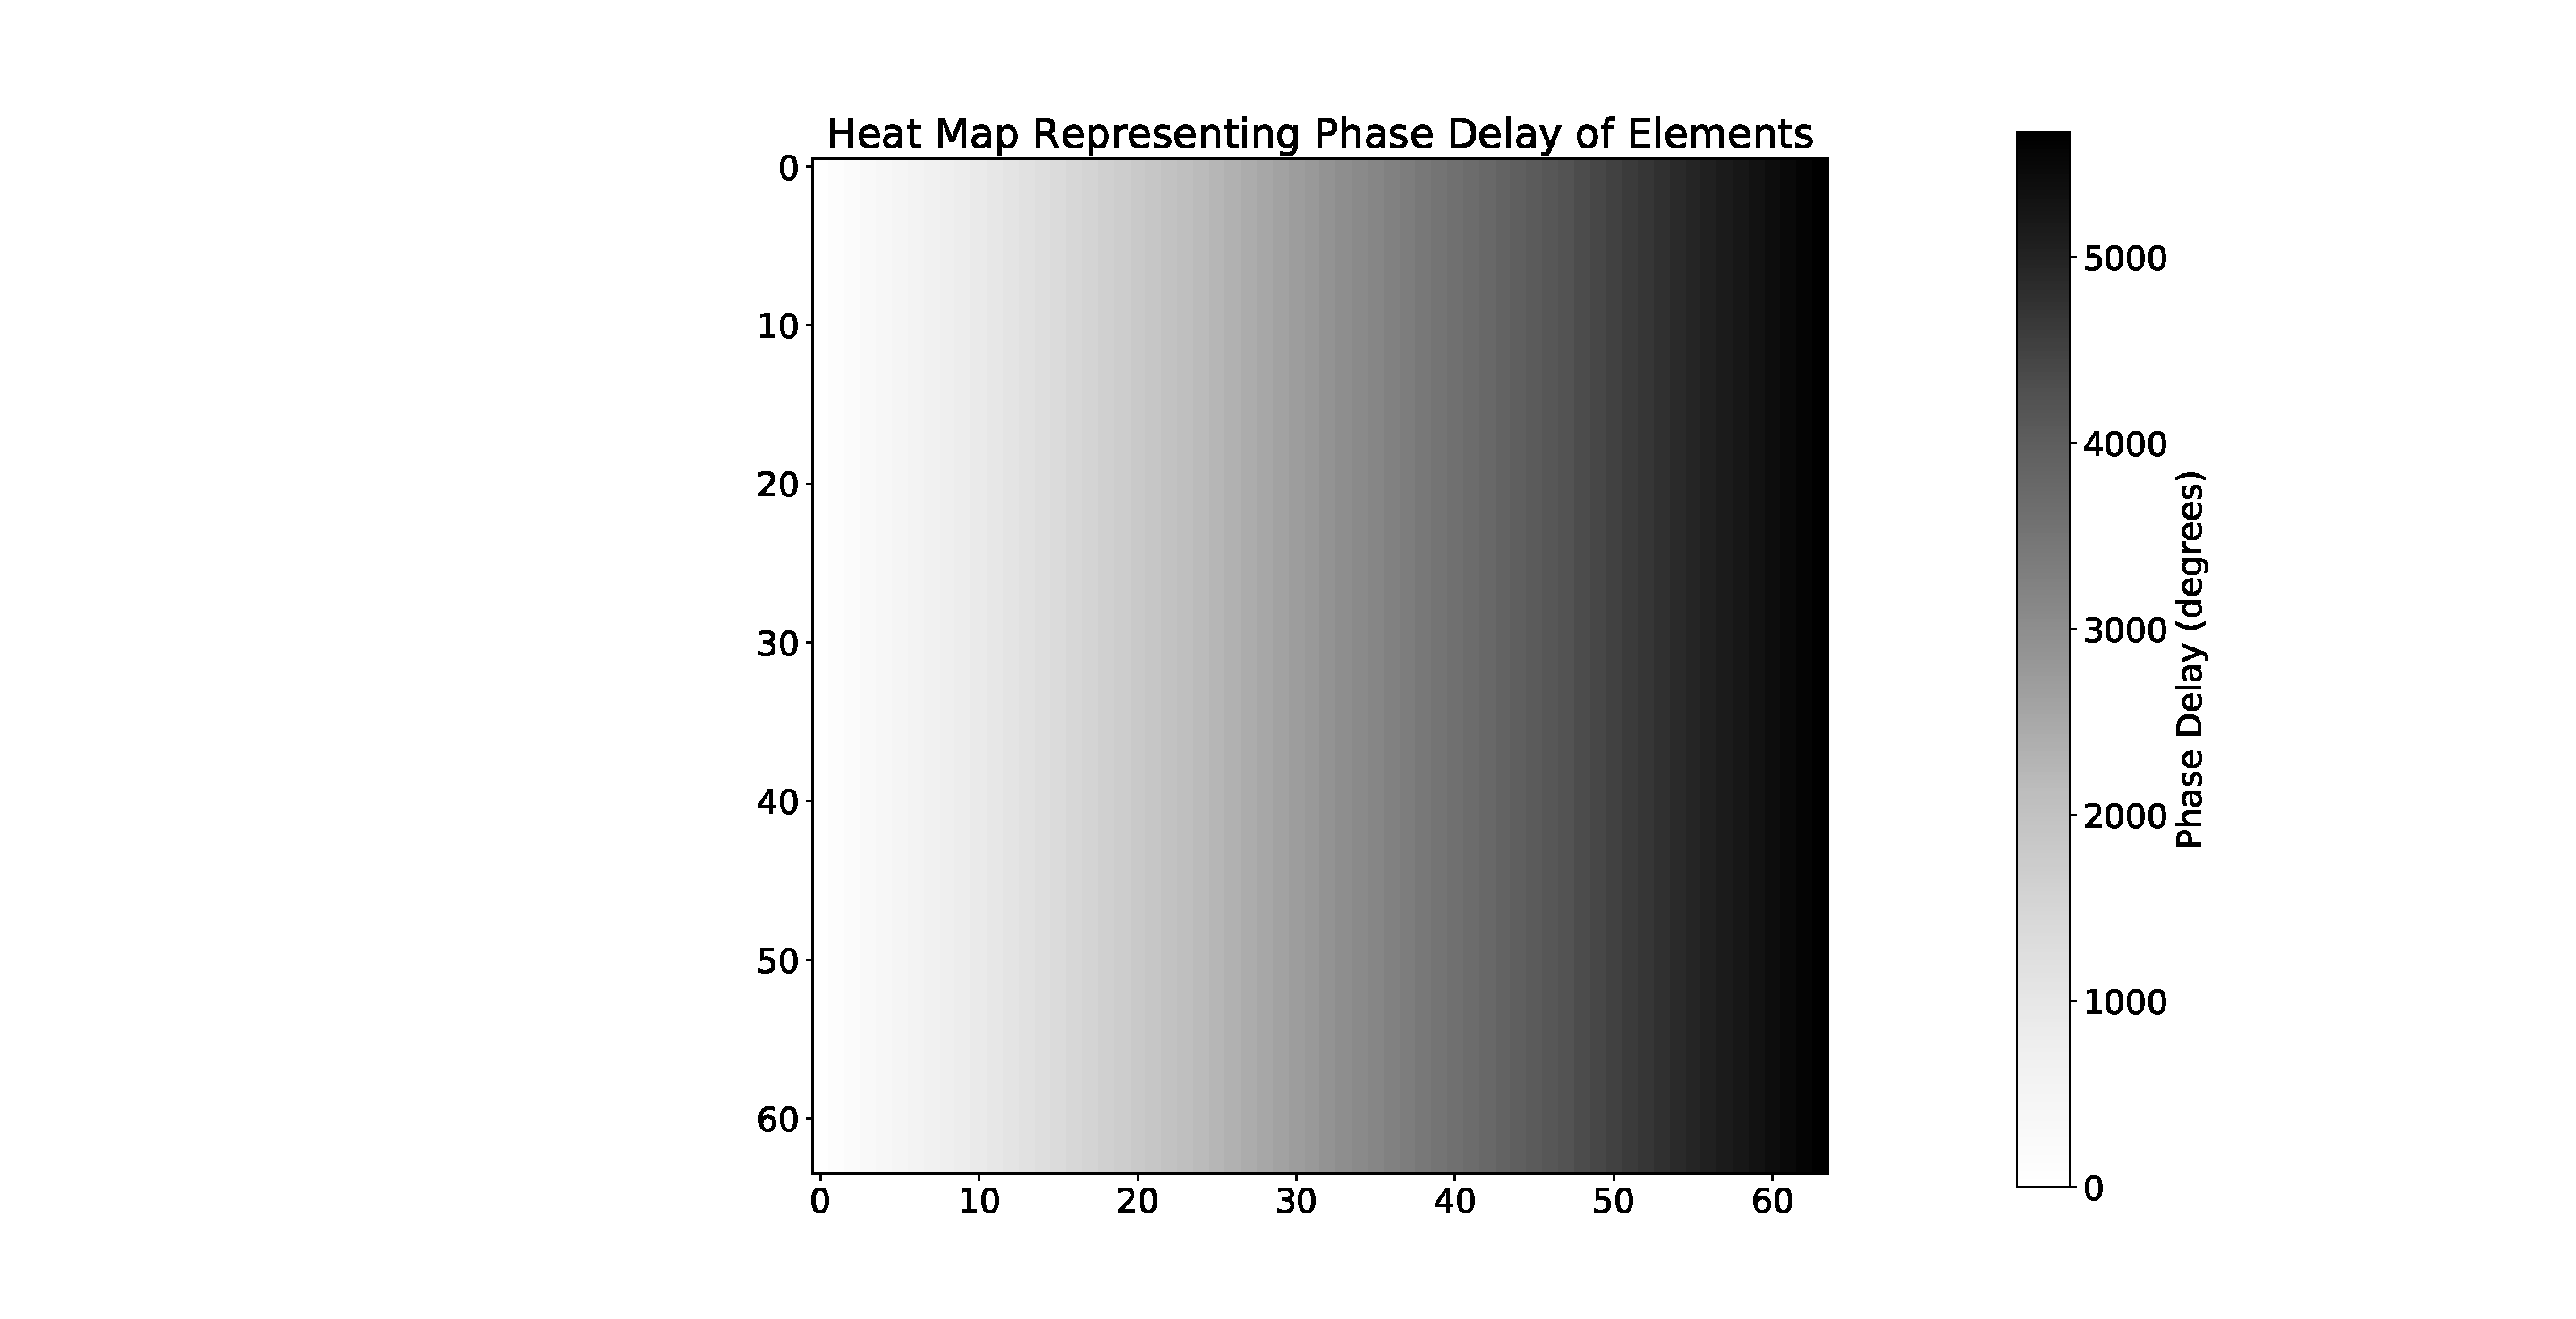
\includegraphics[width=0.9\linewidth]{PhasingHeatMap.pdf}
            \caption{Heat Map Representing the Phase Delay of Each Element}
                \label{fig:PhasingHeatMap}
            \end{subfigure}
\caption{Heat Maps Representing Power Tapering and Phase Delays}
\label{fig:HeatMaps}
\end{figure}

The result of this amplitude excitation is illustrated in Fig.~\ref{fig:PowerTapering} where a uniform $64 \times 64$ array is compared with the tapered $64 \times 64$ array. It is clear from this illustration that there is an increase in side lobe level which results in a more efficient and accurate system. This now reduces the chances of the system detecting objects from the side lobes. 

\begin{figure}[htb]
    \centering
    \begin{subfigure}{.5\textwidth}
        \centering
            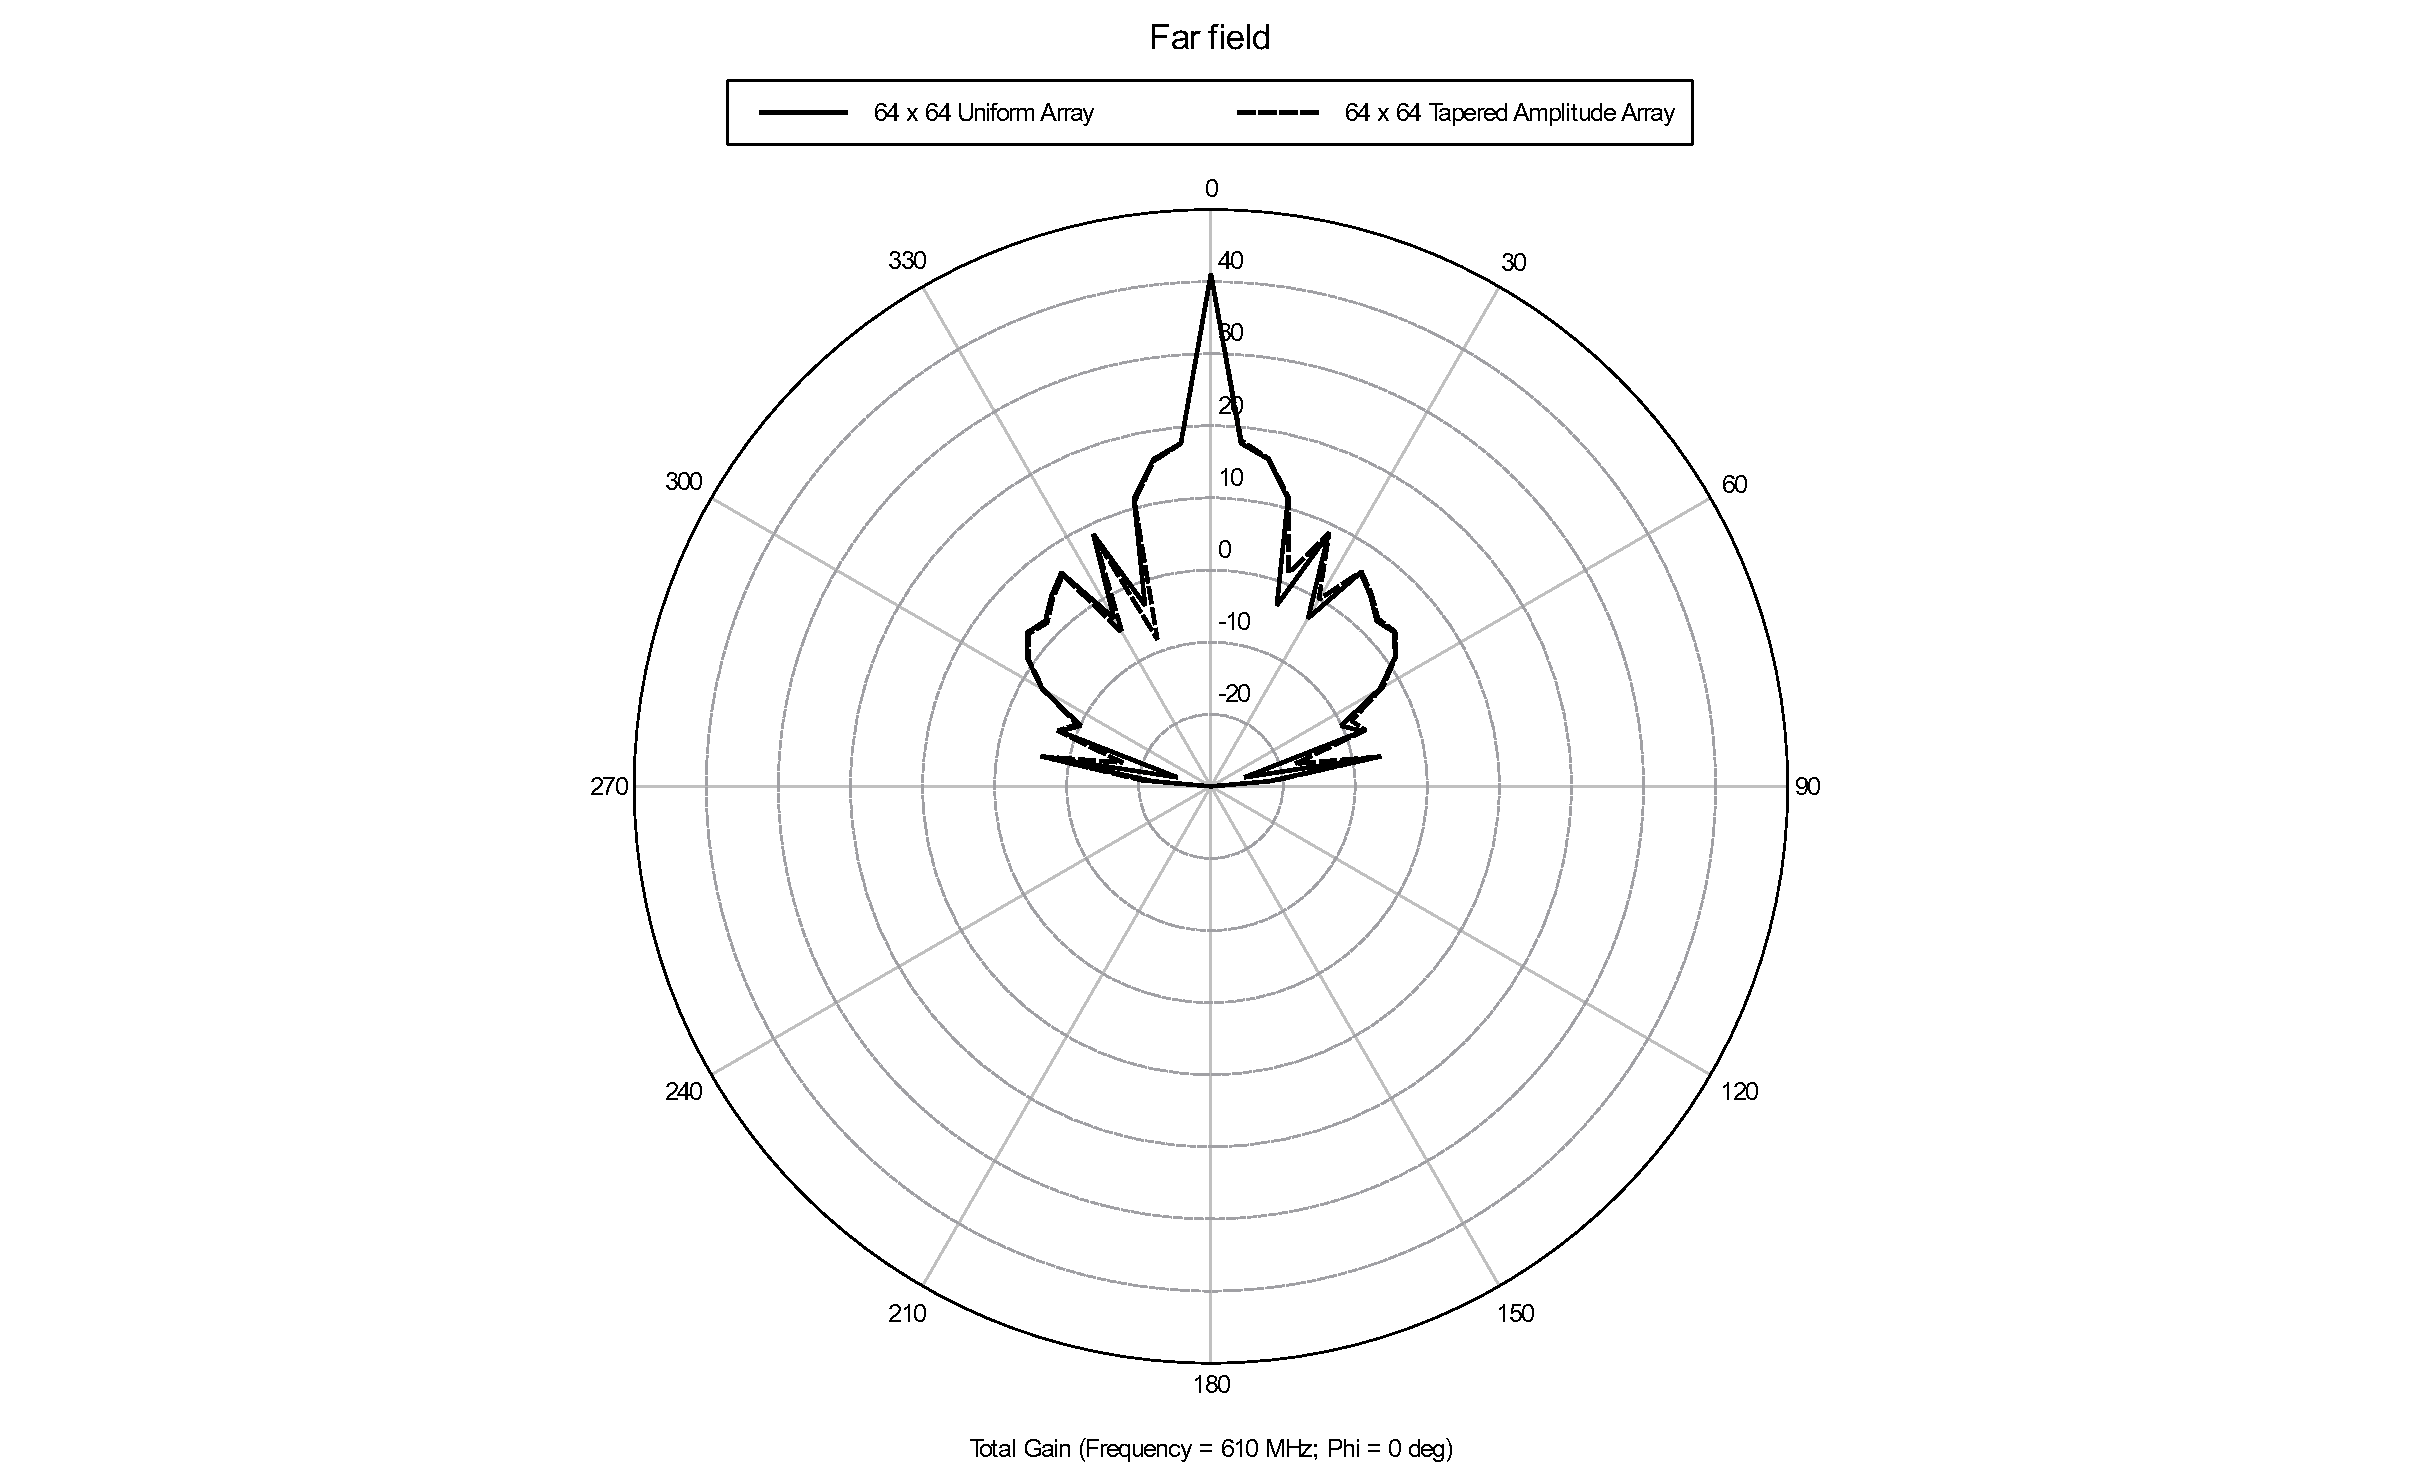
\includegraphics[width=0.9\linewidth]{AmplitudeTapering-Polar.pdf}
            \caption{Uniform vs Tapering - Polar}
            \label{fig:PowerTapering-Polar}
        \end{subfigure}%
        \begin{subfigure}{.5\textwidth}
            \centering
            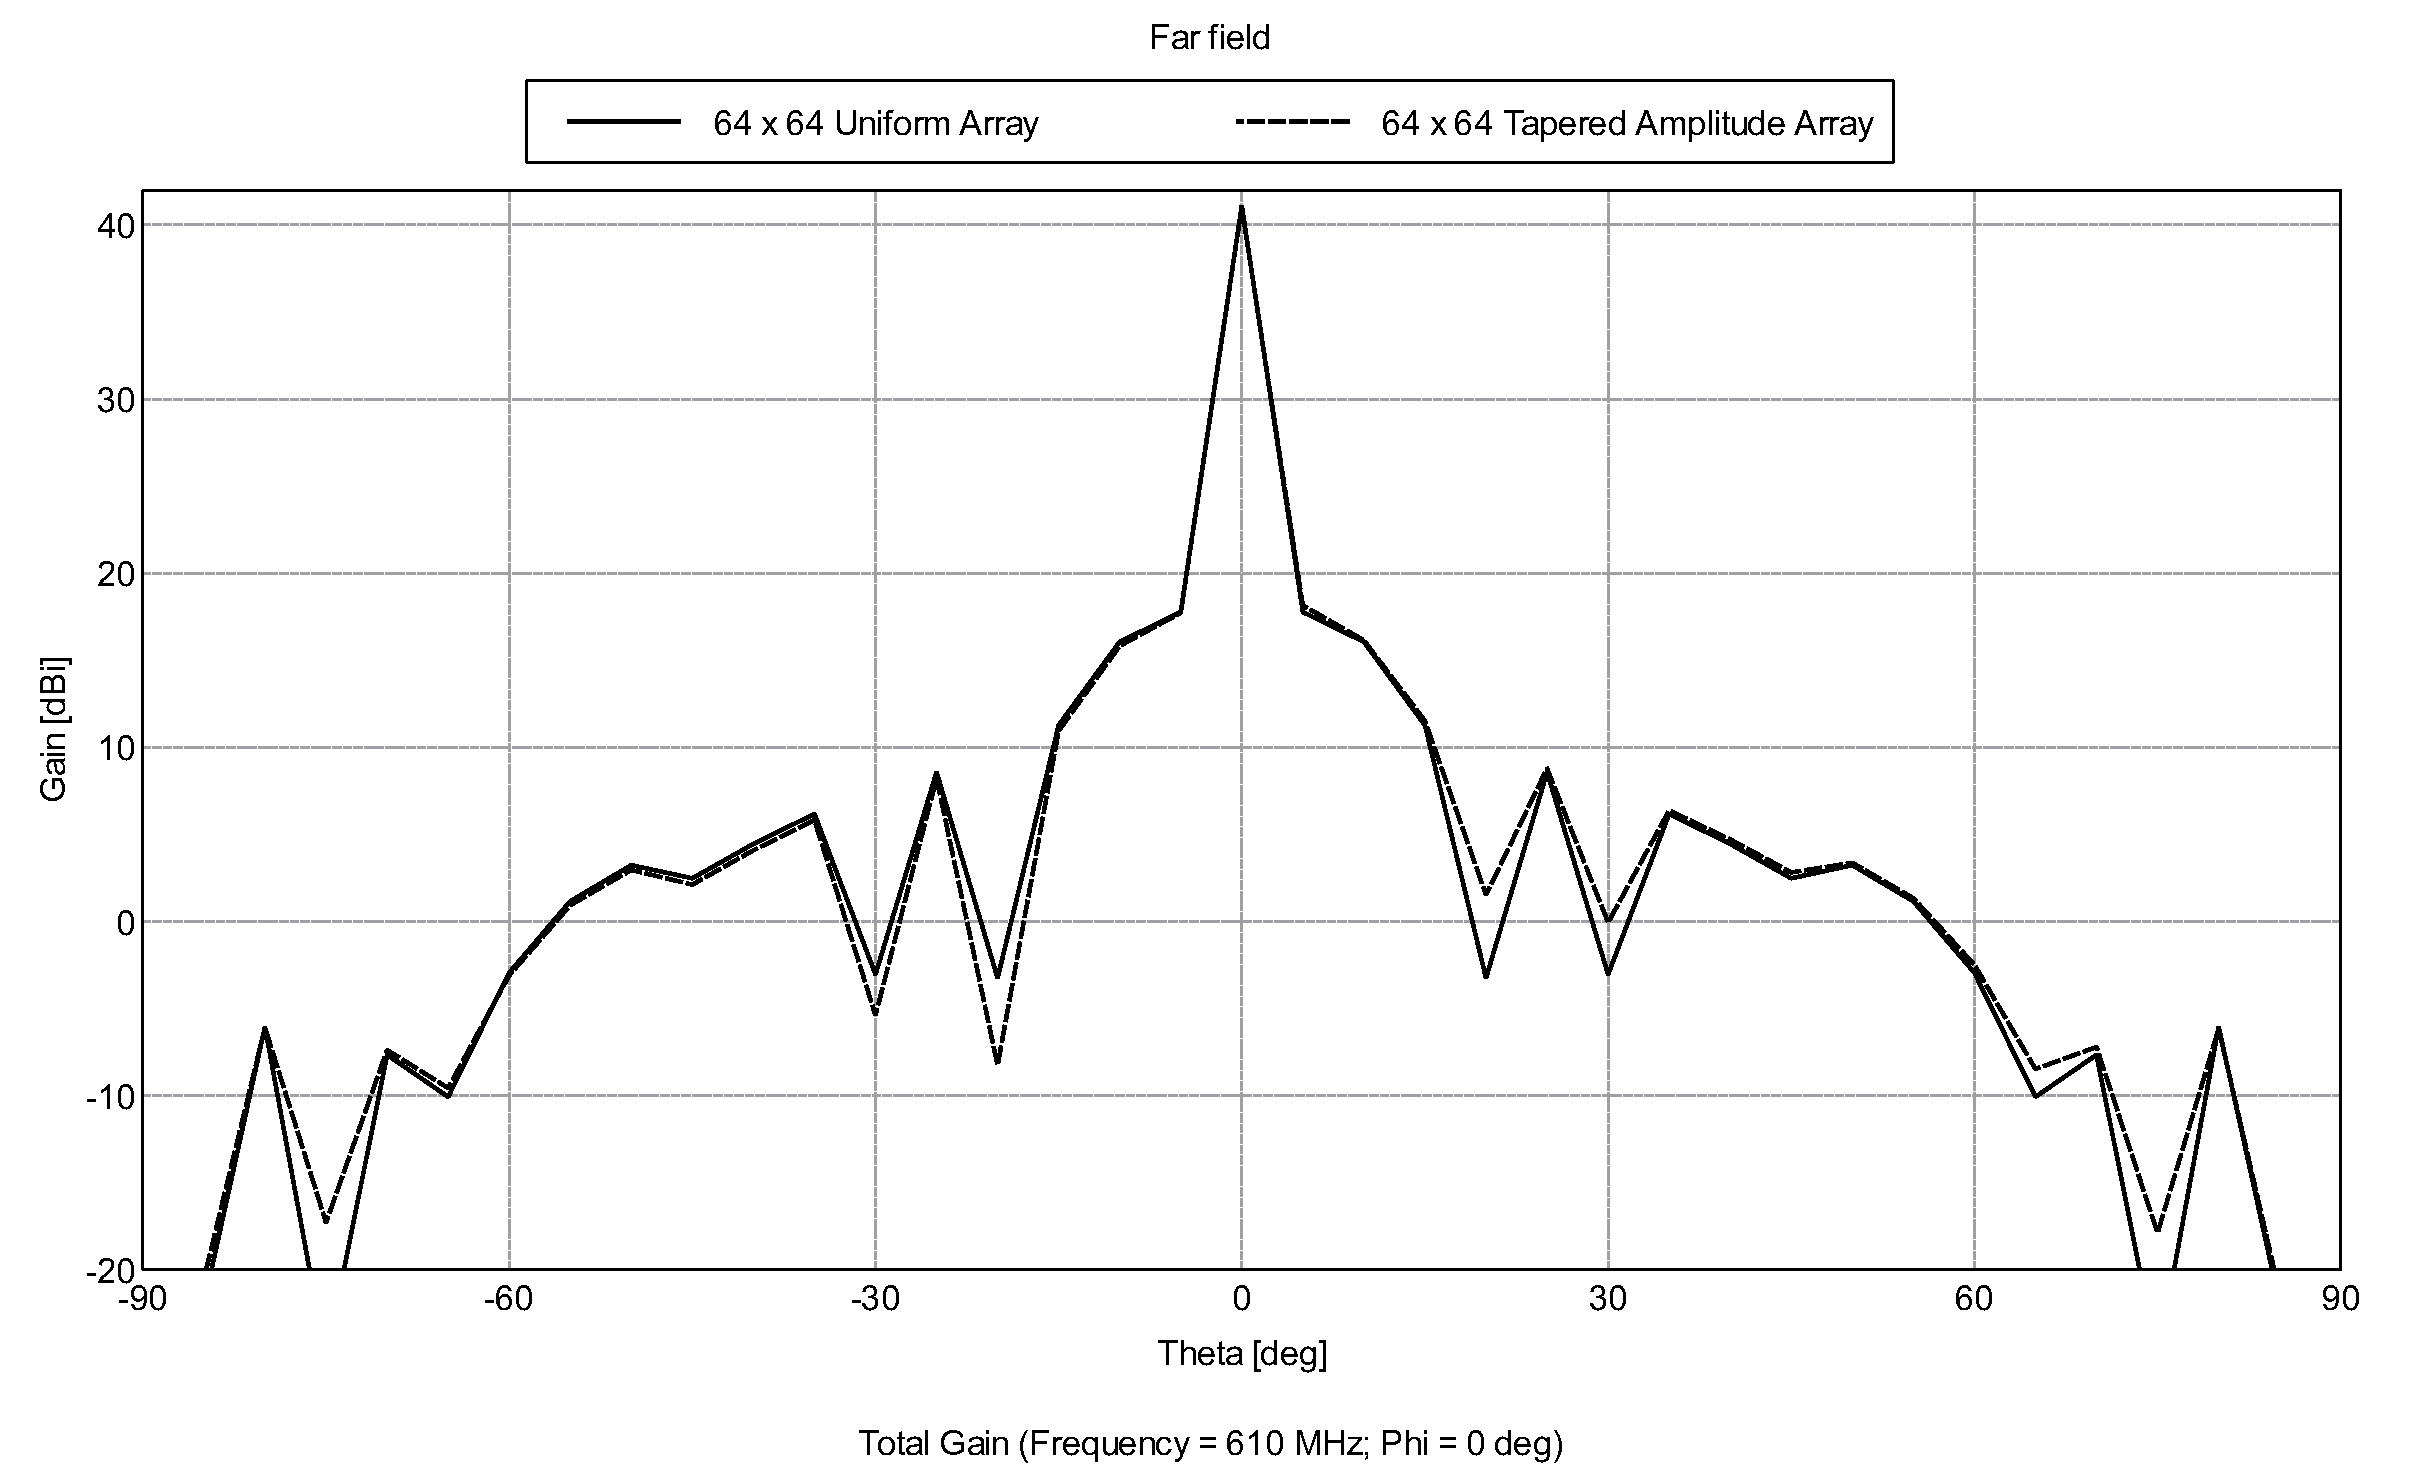
\includegraphics[width=0.9\linewidth]{AmplitudeTapering-Cartesian.pdf}
            \caption{Uniform vs Tapering - Cartesian}
                \label{fig:PowerTapering-Cartesian}
            \end{subfigure}
\caption{Amplitude Excitation with Uniform compared to Tapering}
\label{fig:PowerTapering}
\end{figure}

The result of this tapering is measured and is quantified in table~\ref{tab:AmplitudeTapering}.

\begin{table}[htb]
    \caption{Amplitude Tapering Details}
    \label{tab:AmplitudeTapering}
    \begin{center}
        \begin{tabular}{p{60mm}cp{40mm}cp{40mm}}
            \hline 
            Parameter & Uniform Array & Tapered Array \\
            \hline
            Maximum Gain ($dBi$) & $41.1059$ & $41.0232$ \\
            Maximum Gain Direction (degrees) & $0$ & $0$ \\
            Side Lobe Level ($dB$) & $32.5337$ & $32.2414$ \\
            Half Power Beam Width ($-3 dB$) (degrees) & $1.28995$ & $1.30417$ \\
            \hline
        \end{tabular}
    \end{center}
\end{table}


% \subsection{Radar Functions} \label{sec:RadarFunctions}

% \subsubsection{Search/Detect} \label{sec:SearchDetect}

% \subsubsection{Track} \label{sec:Track}

% \subsubsection{Image} \label{sec:Image}

% \subsubsection{Multi-Pulsing} \label{sec:MultiPulsing}

% Need to talk about how the SNR can be improved with the use of multiple pulses.


% \subsection{Directions} \label{sec:Directions}

% Discuss how the system cannot determine the direction of the object, it can only determine if the object is moving towards the antenna's boresight or away (with an increased doppler freq or a decreased doppler freq)


\subsection{Feeding Networks} \label{sec:FeedingNetworks}
In order to reduce the cost of the overall system, each antenna is designed such that it has its own feeding network. This implies that if a part of a feeding network is damaged, then the only replacement will be for that individual antenna. This makes the system highly modular. 
The feeding network is designed such that each antenna element communicates with a central command module (CMM). This CMM is responsible for the phasing and amplitude selection for each individual antenna element.
The communication between each antenna element is by means of a fibre optic cable. This communications medium reduces the noise on the system as it is not making use of electrical currents which can interfere with the operation of the system. 
This modular system takes is created to be similar to the AMISR \cite{AMISR}, which makes use of modular panels such that there are multiple antennas per module, each module has its own controlling unit, and these controlling units communicate with the CMM.
This implementation is improved in this design based on the newer technology available which allows for higher modularity of the components and higher data communication throughput.
This modular design means that multiple antenna elements can fail with the overall system still functioning sufficiently.

This implementation also results in a simplified feeding mechanism as matching between multiple antennas is no longer required.
The implementation of solid state amplifiers is used here as they are highly reliable, easily maintainable, and are modular in nature. The down side of solid state amplifiers is that they are not able to generate large amounts of power \cite[p.~364]{radarHandbook}, however, due to the fact that the power is split between each element in the array, they are ideally suited to this application. The implementation of solid state technology results in the use of DC voltages throughout the system, this is an important factor for this implementation as DC creates minimal interference to the antennas.
The implementation of modular components means that the only cabling required throughout the array will be the DC power cables for the element modules and communication lines. These two lines do not interfere with each other as the communication lines are fibre optic and so are unaffected.
Consequently, the radiating elements are located within the element module and the connector cables from the module to the antenna.
The interference from the electronics within the module can be reduced with the use of shielding the walls of the module. The connector cables make use of sleeve baluns which reduce the radiating components commonly seen on coaxial cables.

\subsubsection{Transmitter} \label{sec:Transmitter}

\subsubsection{Receiver} \label{sec:Receiver}
The frequency utilised within this system is relatively large when considering the Analogue-to-Digital-Converters (ADC) currently available. The cost of ADC components which are capable of sampling this frequency are prohibitively expensive.
This calls for the use of a frequency mixer (down-converter) such that the EM waves received by the amplifier are shifted down in frequency and are then sampled at that point. Once this sampling has taken place, processing of the data takes place to determine if detection has occurred.
This implementation reduces the cost of each receiver system. The overall diagram of this is illustrated in Fig.~\ref{fig:ReceiverDiagram}. The transmitter part of the system is illustrated here as a block as it interacts with the system through the circulator. The local oscillators frequency is required to be relatively close to that of the system as the intermediate frequency (IF) output from the mixer \cite[p.~397-398]{radarHandbook}. 
The implementation of a second mixing stage decreases the mixers intermodulation components which allows for easy filtering (removal) to get the final signal \cite[p.~398]{radarHandbook}.
The lower frequency signal created from this process is then easily sampled with a lower cost, high quality, ADC such that characterisation of the signals is possible. The detail of the mixing process is out of the scope of this design as the final IF frequency for sampling requires further calculation.

\begin{center}
    \begin{figure}
        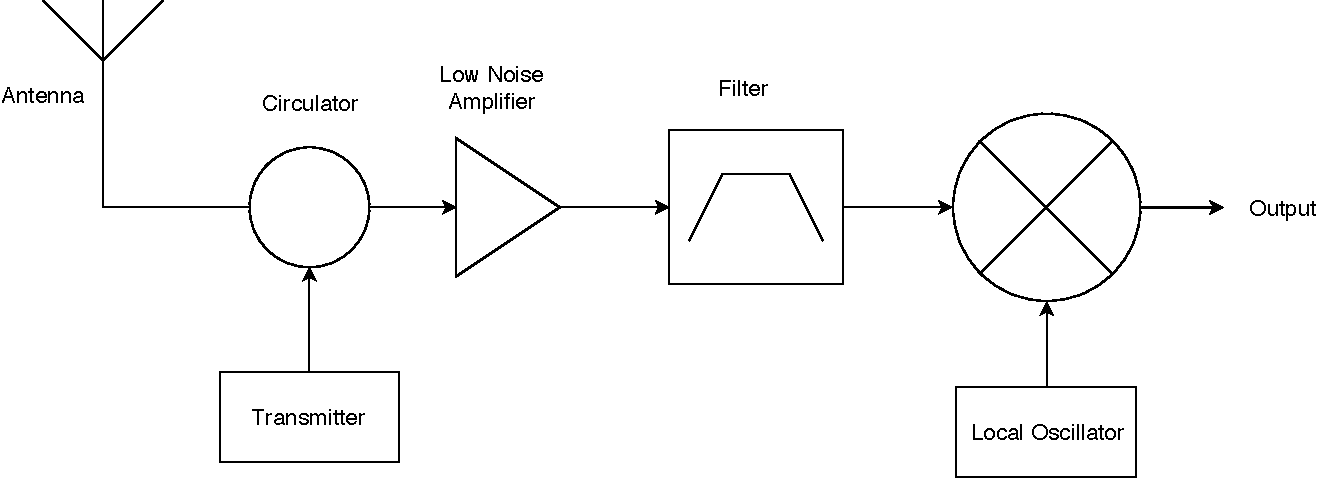
\includegraphics[width=\textwidth]{ReceiverDiagram.pdf}
        \caption{Receiver Diagram}
        \label{fig:ReceiverDiagram}    
    \end{figure}
\end{center}
The LNA is placed close to the physical antenna as this lowers the noise introduced via the transmission medium. Efficient placement of these components components is required for this 


***

Speak about how the signals are put together further down the line (with the use of maximum ratio combining)

Wilkinson splitter

Circulator
Corporate feed

\subsection{Mixer} \label{sec:Mixer}


\section{Environmental Considerations} \label{sec:EnvironmentalConsiderations}
The design of this system has considered the technical details of tracking space debris. In order to implement this in a real world situation the environmental factors are analysed in this section.
% Based on the choice of the frequency and how it is used, the location of the system is based in the Northern Cape where there is a low population density and a large area. This is highly important such that the system has as little radio interference as possible.

\subsection{Location} \label{sec:Location}
Subject to the choice of the frequency and how it it licensed, the array is situated within the Northern Cape (refer to section~\ref{sec:OptimalFrequency}). This is based on the fact that the SKA has the ability to provide a number of laws which allow for the selected frequency to be utilised within this province.
The Northern Cape is a largely unpopulated area when compared to the rest of the country, implying that it has a low population density (as it has the largest area). This is convenient as it lowers the cost per area of land. 
Based on the spacing of the array, the size of land required should be at least $247~m^2$ (based on the $\Lambda/2$ spacing and the $64 \times 64$ array sizing), this is the minimum area required for the placement of the antennas. The system is equipped with a number of additional components which all take up space.
This implies that the system is required to be able to be housed with at least a $2000~m^2$ plot of land, this implies that, based on the average cost of units of land of this size, the price will be approximately $R~800~000$ to $R~1~200~000$ \cite{LocationPrice1, LocationPrice2, LocationPrice3}.
The price of the plot of land varies based on its location, previous owners, and proximity to towns. A pragmatic approach to estimating the cost of the required land is to take the maximum value stated here and add on an additional $20~\%$. The cost of the area of land is then approximated to $R~1~440~000$.

The ideal location for the land would be within a short distance from the SKA operations, this results in the added benefit of the lowered radio interference from external sources while being able to cooperate with their operations. 
The SKA has currently build their own infrastructure for data management. Tying in with their system implies a lower cost for both parties as it can benefit both. The cost incurred for this communication platform can become expensive, an in-depth analysis should be undertaken as to how the data transmission mechanism should work.
The first method is to make use of on-site servers which take all of the information directly from the array and apply analysis on this data, package the data, and send out the important characteristics that it has analysed. The second method is to automatically send out all of the data that is retrieved from the system, this data is then sent directly to an external server (a cloud provider such as Google, Amazon, etc.) and then the analysis is then carried out from this service.
The cost of these two systems are required to be analysed as they both have benefits and drawbacks.
The first method will require a large up front investment for the installation of the servers, then an recurring cost for the energy that is consumed for the analysis, this greatly reduces the costs of data transmission.
The second method will have minimal up front costs, other than the recurring cost of the maintenance and rental of the data line, as well as the costs to analyse this data when it is stored on the cloud.
The SKA ran a feasibility study to determine which of these methods is more cost efficient, their decision was to install an on-site data center as the costs of installing a fibre line to transport the data far exceeded the installation costs of the data center \cite[p.~17-18]{SKAFibre}.
This data center will require the installation of an RFI shielded building such that the components inside do not interfere with the array \cite[p.~18]{SKAFibre}.

The power requirements for the installation of this system can become complex, in addition to this, the power transmission system should comply with the regulations of the SKA. The SKA undertook an investigation to the installation for power \cite{SKAFibre}, this document highlight the requirements for the installation of power and how it is required to be routed.


The plot of land is required to be relatively low gradient for the installation of the physical array as this is required to be mounted flush against the surface of the Earth and directed upwards.
In order to install the system, an in depth analysis is required to be carried on the land, this analysis includes has been undertaken by the SKA in the local area ($180~km$ radius)\cite[p.~95,98]{SKAFibre}, which concludes that the minimum depth at which the structure can be fixed is $3.5~m$ below the surface. The nature of the ground under the array can prove to be difficult to lay foundations for construction.

Due to the placement of the SKA, placing the system in close proximity implies that low flying aircraft are prohibited within the local airspace as this can affect the system.
Local authorities should be notified of the implementation of this system such that regulations are put in place for flight paths that may be affected.

Depending on the site chosen, roads and standard infrastructure (water, electricity, etc.) may be required for the construction of the system, this increases the overall cost.

This system should be capable of functioning for a minimum of $40$ years \cite[p.~336]{AMISRCosting}, this is a standard requirement for large operations, as such it should be capable of withstanding the environment for this period of time. Section~\ref{sec:WeatherDependence} analyses a number of concerns for the area of installation.

\subsection{Weather Dependence} \label{sec:WeatherDependence}
The Northern Cape (specifically near Carvernon, where the SKA is situated) is at a relatively high altitude, it is also a semi-arid area with little rainfall throughout the year \cite{Rainfall}.
This is highly beneficial for the system as rainfall can severely affect the functioning of the system (due to the loss of EM wave energy by the water).
The low humidity and rainfall is convenient for this system as this area is located above the rust belt (the border where corrosion from the sea air is reduced to negligible levels) of South Africa which. This implies that the system will require little to no maintenance from corrosion over time.

The temperatures experienced during the Summer season in this area of the country often range between $34$ to $40^{\circ} C$. Frost and dew often occur during the winter months, this implies that the components should be designed such that they can handle extreme temperature swings.

\section{Construction} \label{sec:Construction}

How things fit together, how the cables are placed
What kind of cables
What communications medium is used between modules



\section{Costing Analysis} \label{sec:CostingAnalysis}

In order to estimate the total cost of the system, previously implemented systems that have a similar functionality can be compared. The first of these is the EISCAT Svalbard Radar Project \cite[p.~670]{EISCATPrice} which estimated the cost of the project to have cost approximately $R~432~000~000$ in $1995$, and the yearly operating costs approximated $R~40~000~000$. This cost is indicative of the technology at the time and these costs will be greatly reduced with the use of newer efficient technology.
The estimate for the entire solid-state amplifier implementation was estimated to be $R~300~000~000$, this includes the cooling, control systems, and transmitter modules. This is a high estimate as the cost of this will have been reduced over time.

The second comparable system is that of the AMISR (used by Leo Labs), which is estimated, once construction was completed to cost approximately $\$52$ million ($R~750$ million) for the concept development and implementation \cite[p.~333-337]{AMISRCosting}. The yearly operational cost for the system is estimated to be approximately $\$3$ million ($~R43$ million). This estimate is closer to the cost requirements for this design as the systems are constructed with a number of similarities for the components.
The use of solid state amplifiers appears to be the best choice as the price of these components have decreased over the past two decades and their efficiency has increased while increasing the average output power.
The Design document has a number of costing estimates for solid state amplifier implementation, however, this estimate was in 1990 \cite[p.~37]{DesignDraft}.
Table~\ref{tab:CostingUnit} illustrates the costing for an individual unit, this includes the antenna, transmitter and receiver components. The exchange rate is taken as $R~14.40/\$$.
Based on average prices of antennas which have similar characteristics \cite{AntennaPrice1,AntennaPrice2,AntennaPrice3,AntennaPrice4,AntennaPrice5}, the cost estimate for the antenna is chosen to be approximately $R~10~000$, which is a high estimate, however, this takes into consideration the requirements for the antenna to have a high tolerance, high power capability, low VSWR, and high efficiency. The communications unit is required to communicate with the CMM such that the antenna that it is connected to is operated in the required way. This system is housed within the antenna module as it should be shielded from the antenna and surrounding equipment. The estimate for the component is set at $R~20~000$. The control unit is responsible for communicating the information between the communication module and the electronics within the system, this system is costed at $R~15~000$.

\begin{table}[htb]
    \caption{Antenna Module Costing}
    \label{tab:CostingUnit}
    \begin{center}
        \begin{tabular}{c c c c c}
            \hline 
            Component & ID & Number & Unit Price ($R$) & Amount ($R$) \\
            \hline
            Antenna & $N/A$ & $1$ & $10~000~000$ & $10~000~000$ \\
            Control Unit & $N/A$ & $1$ & $15~000$ & $15~000$ \\
            Communication Unit & $N/A$ & $1$ & $20~000$ & $20~000$ \\

            LNA & $ZHL-100-3W+$ \cite{LNA} & 1 & $10~008$ & $10~008$ \\
            Filter & $SXBP-640+$ \cite{Filter} & $2$ & $258.48$ & $516.96$ \\
            Mixer & $TUF-R5SM+$ \cite{Mixer} & $1$ & $186.48$ & $186.48$ \\
            SMA Connectors & $35F-35M50+$ \cite{SMA} & $5$ & $935.28$ & $4676.4$ \\
            Cables & $141-10SM+$ \cite{Cables} & $5$ & $136.66$ & $683.28$ \\
            DC Blocker & $BLK-89-S+$ \cite{DCBlocker} & $1$ & $215.28$ & $215.28$ \\
            Oscillator & $Z0S-765+$ \cite{Oscillator} & $1$ & $1727.28$ & $1727.28$ \\
            Circulator & $SKYFR-000736$ \cite{Circulator} & $1$ & $143.28$ & $143.28$ \\  
            \hline
            \textbf{Total} & & & & \textbf{$63~146.96$} \\ 
            \hline
        \end{tabular}
    \end{center}
\end{table}
This implies that the cost of the array, purely from the antenna element units is estimated to be approximately $R~258~650~000$. This estimate is close to that of the EISCAT implementation as it is within $20\%$ of their estimate for the antenna system.
This costing does not take into consideration the price of the installation of the data center, roads, water supply, electricity supply, control rooms, land, etc. It is assumed that the cost of these contribute to twice the value of the array.
This means that the total cost of the system can be estimated to approach $R~775~950~000$.


\section*{ACKNOWLEDGEMENT} \label{sec:ACKNOWLEDGEMENT}





\bibliographystyle{witseie}
\bibliography{references}

\newpage
\onecolumn
\pagenumbering{roman}
\setcounter{page}{1}
\setcounter{figure}{0} 
\renewcommand{\thefigure}
{A\arabic{figure}}

% APPENDICES
\onecolumn
\appendix

\section{Social, Economic, and Environmental Implications}

\subsection{Social Implications} \label{sec:SocialImplications}
Benefit to the research institutions and science as a whole.
Employment of nearby townsfolk


\subsection{Economic Implications} \label{sec:EconomicImplications}
Benefit to the launching of satellites

Employment of nearby townsfolk


\subsection{Environmental Implications} \label{sec:EnvironmentalImplications}
Frequency introduction into atmosphere and surrounding areas
Destruction of desert slug populations
Destruction of arid zone bos

Requirement of water in an already dry place
Electricity requirements
Lead free stuffies



\section{Background to Space Debris} \label{sec:BackgroundToSpaceDebris}
This was not thought to be an issue to the world at large as the belief was that space is immense and so there were no issues with using it as a dumping ground. It was not until the realisation by Kessler that the world began to worry \cite{Kessler}. This theory predicted that as the number of man made satellites (and other objects) in Earth's orbit increases, so does the probability of collisions between them increase. When orbiting debris collide, the two objects can fragment (due to the excessive relative speeds with which the two objects travel at) and case multiple cascading collisions. This means that the debris orbiting the Earth would increase and result in greater difficulty for active space craft to undertake their missions.
Protecting active missions from this space debris is highly difficult as it is difficult to predict the density of objects in the specific orbit that the missions' device should be in.

Guidelines were developed by NASA in the late 70's, however, this simply slowed the rate of introduction of debris, this did nothing to reduce the currently orbiting debris \cite{spaceDebrisGuide}. Recently, the United Nations General Assembly managed to get agreement between a number of countries to reduce the introduction of this debris \cite{debrisGuidelinesAgreement}.

There have been a number of methods in which to deal with this issue. The first is to protect the current missions from this debris, in this case, make use of a Whipple shield, this is simply an outer coating of space craft that is able to protect the craft against high velocity impacts of objects in outer space \cite{Whipple}. This shield is built to protect the craft from impacts from micrometeoroids in space.
This method falls short when the debris becomes large enough to penetrate the craft (and the Whipple shield), resulting in the destruction/damage of the craft.

A recent system is capable of removing debris from the Earth's orbit, however, this is still in its early stages and has yet to prove highly effective \cite{removalSpaceDebris}.

\section{Coordinate System} \label{sec:CoordinateSystem}
The coordinate system used throughout this design report the coordinate system used is illustrated in Fig.~\ref{fig:CoordinateSystem}, this is the spherical coordinate system.
\begin{figure}
    \centering
%Angle Definitions
%-----------------

%set the plot display orientation
%synatax: \tdplotsetdisplay{\theta_d}{\phi_d}
\tdplotsetmaincoords{60}{110}

%define polar coordinates for some vector
%TODO: look into using 3d spherical coordinate system
\pgfmathsetmacro{\rvec}{.8}
\pgfmathsetmacro{\thetavec}{30}
\pgfmathsetmacro{\phivec}{60}

%start tikz picture, and use the tdplot_main_coords style to implement the display 
%coordinate transformation provided by 3dplot
\begin{tikzpicture}[scale=3,tdplot_main_coords]

%set up some coordinates 
%-----------------------
\coordinate (O) at (0,0,0);

%determine a coordinate (P) using (r,\theta,\phi) coordinates.  This command
%also determines (Pxy), (Pxz), and (Pyz): the xy-, xz-, and yz-projections
%of the point (P).
%syntax: \tdplotsetcoord{Coordinate name without parentheses}{r}{\theta}{\phi}
\tdplotsetcoord{P}{\rvec}{\thetavec}{\phivec}

%draw figure contents
%--------------------

%draw the main coordinate system axes
\draw[thick,->] (0,0,0) -- (1,0,0) node[anchor=north east]{$x$};
\draw[thick,->] (0,0,0) -- (0,1,0) node[anchor=north west]{$y$};
\draw[thick,->] (0,0,0) -- (0,0,1) node[anchor=south]{$z$};

%draw a vector from origin to point (P) 
\draw[-stealth,color=black] (O) -- (P);

%draw projection on xy plane, and a connecting line
\draw[dashed, color=black] (O) -- (Pxy);
\draw[dashed, color=black] (P) -- (Pxy);

%draw the angle \phi, and label it
%syntax: \tdplotdrawarc[coordinate frame, draw options]{center point}{r}{angle}{label options}{label}
\tdplotdrawarc{(O)}{0.2}{0}{\phivec}{anchor=north}{$\phi$}


%set the rotated coordinate system so the x'-y' plane lies within the
%"theta plane" of the main coordinate system
%syntax: \tdplotsetthetaplanecoords{\phi}
\tdplotsetthetaplanecoords{\phivec}

%draw theta arc and label, using rotated coordinate system
\tdplotdrawarc[tdplot_rotated_coords]{(0,0,0)}{0.5}{0}{\thetavec}{anchor=south west}{$\theta$}

%draw some dashed arcs, demonstrating direct arc drawing
\draw[dashed,tdplot_rotated_coords] (\rvec,0,0) arc (0:90:\rvec);
\draw[dashed] (\rvec,0,0) arc (0:90:\rvec);

%set the rotated coordinate definition within display using a translation
%coordinate and Euler angles in the "z(\alpha)y(\beta)z(\gamma)" euler rotation convention
%syntax: \tdplotsetrotatedcoords{\alpha}{\beta}{\gamma}
\tdplotsetrotatedcoords{\phivec}{\thetavec}{0}

\end{tikzpicture}
\caption{Coordinate System}
\label{fig:CoordinateSystem}
\end{figure}


\subsection{Space Debris Parameters} \label{sec:SpaceDebrisParameters}
As discussed in section~\ref{sec:INTRODUCTION}, space debris in Earth's orbit has been increasing for many decades, this is mainly due to space missions with poor regulations on the material that is allowed to stay in Earth's orbit.
The majority of space debris currently is made up of man made air craft components, this includes objects such as: functioning space craft, non-functional spacecraft, rocket bodies, exhaust products, objects created through deployment operations, and products of deteriorated space craft \cite{OrbitalDebrisTechnicalAssessment}.
Consequently, a large amount of this debris is made up of metallic materials as these materials make up the majority of the space crafts' components.
It has, in the past \cite{Spacex}, been difficult and costly to retrieve the components which were used to get the space craft into orbit, this is a major contributor to the material.
This debris can occupy a number of regions within the Earth's orbits and this changes its characteristics.

The current scope of the project is that it should be capable of tracking space debris that is within the Low Earth Orbit (LEO). This orbit is defined to be approximately $160 km$ to $2000 km$ altitude above the Earth's mean sea level.


\subsubsection{Space Debris Trajectory Characteristics} \label{sec:SpaceDebrisTrajectoryCharacteristics}

The second definition of these orbits is baed on orbital mechanics, this states that if an object is within an orbit, then it will have a corresponding velocity.
This is illustrated by equation~\ref{eqn:OrbitalVelocity}. 

\begin{equation} \label{eqn:OrbitalVelocity}
    V_{Object} = \sqrt{\frac{G M_{Earth}}{r_{Earth} + r_{Altitude}}}
\end{equation}
Where:
\begin{itemize}
    \item $V_{Object}$ is the radial velocity of the object
    \item $G$ is the gravitational constant ($6.67408 \cdot 10^{-11} m^3 kg^{-1} s^{-2}$)
    \item $M_{earth}$ is the mass of the Earth ($5972 \cdot 10^{24} kg$)
    \item $r_{Earth}$ is the mean radius of the Earth
    \item $r_{Altitude}$ is the altitude of the object above the mean radius of the Earth
\end{itemize}

This allows for the simple calculation of the minimum and maximum orbital speeds expected from the objects which correspond to the maximum altitude and minimum altitude respectively. These are illustrated in table~\ref{tab:ObjectParameters}. The velocity in the table is stated as a tangential velocity as it is assumed that the radial velocity of the object is zero. If an object has a radial velocity component, then this implies that it is changing orbits (an object in a specified orbit will have zero radial velocity) and this is either taking place due to a force acting on the object (man made) or it is experiencing a force due to the Earth's atmosphere. The vectors which explain this movement of an object is illustrated in Fig.~\ref{fig:ObjectVelocityVectors}.

\begin{figure}[htb]
    \centering
    \begin{subfigure}{.5\textwidth}
        \centering
            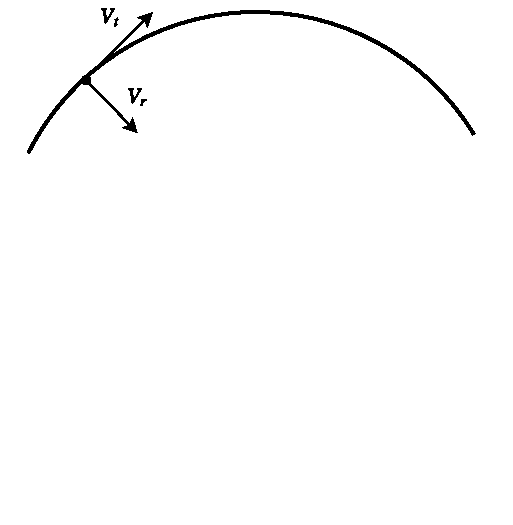
\includegraphics[width=0.9\linewidth]{Vectors.pdf}
            \caption{Object Velocity Vectors}
            \label{fig:ObjectVelocityVectors}
        \end{subfigure}%
        \begin{subfigure}{.5\textwidth}
            \centering
            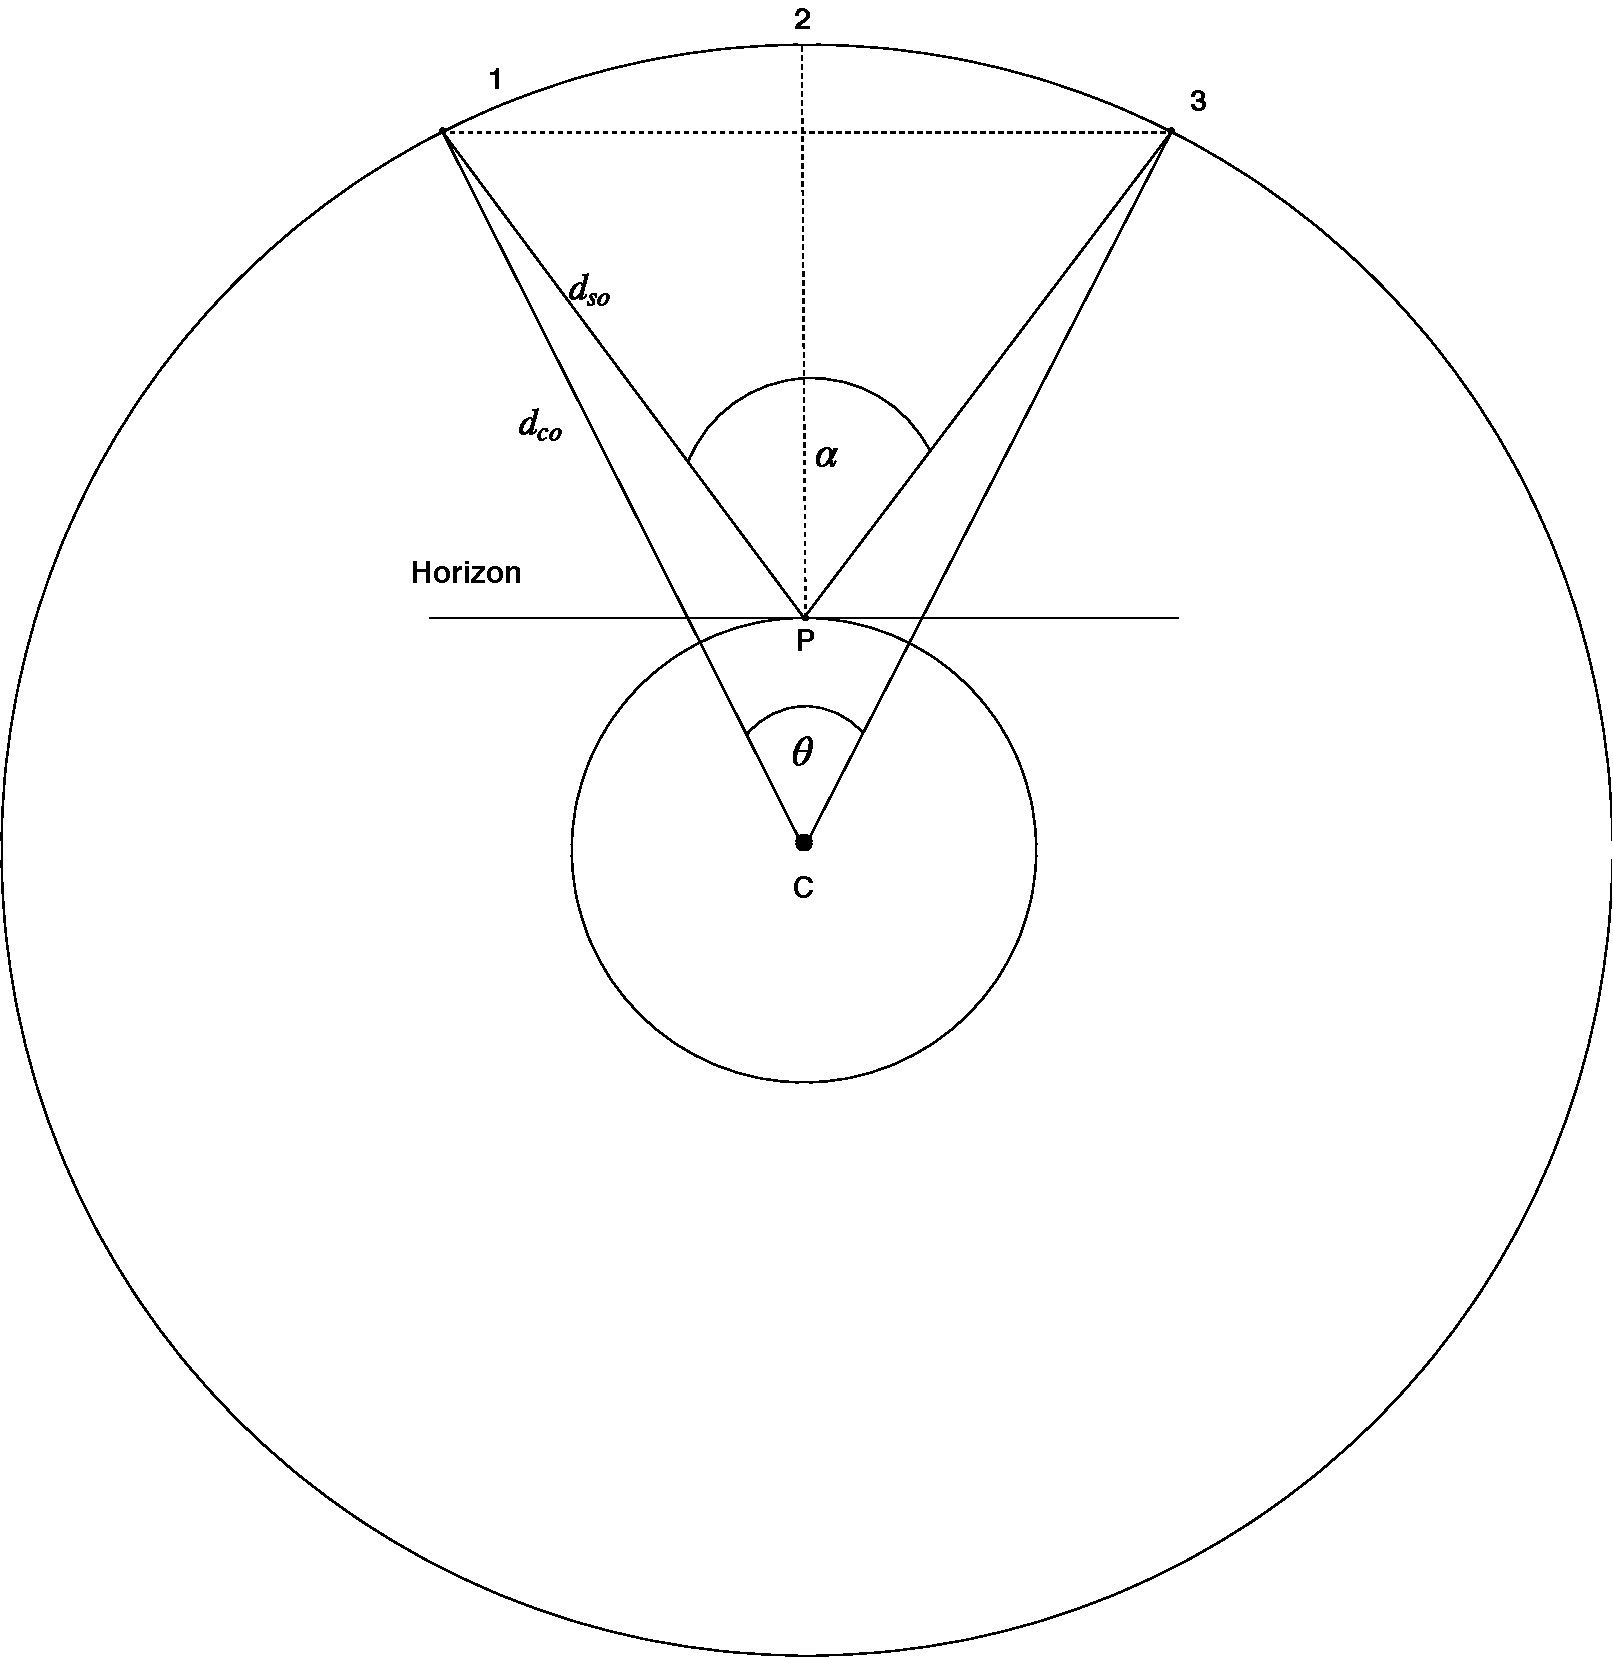
\includegraphics[width=0.9\linewidth]{ObservableCharacteristics.pdf}
            \caption{Observable Characteristics}
                \label{fig:ObservableCharacteristics}
            \end{subfigure}
\caption{Object Characteristics}
\label{fig:ObjectCharacteristics}
\end{figure}


The objects orbiting within these ranges have corresponding periods (amount of time it takes for an object to orbit around the Earth once), this means that an object in the lower orbit has a higher period than that of the higher orbits. The periods for the two limits of the LEO objects are also found in table~\ref{tab:ObjectParameters}.

Based on a number of physical limitations, the system implemented is only capable of detecting the space debris once it appears within the field of view (FOV). The FOV is discussed in section~\ref{sec:FieldofViewandBeamDirection}. Fig.~\ref{fig:ObservableCharacteristics} illustrates the system and its relation to the Earth.
The inner circle represents the Earth's surface and point P represents the position of the system on the Earth's surface.  
The outer circle represents the path of an object orbiting the Earth.
The lengths in this image are not to scale and do not represent the real situation, however, this is used for illustrative purposes.
It is highly important to determine the amount of time it takes from when the object first enters the systems FOV, until the point where it exits the systems point of view.
In this case it is assumed that the object travels directly over the boresight of the system and so it will take the maximum amount of time to travel over the field of view. In most cases, the objects do not travel directly over the FOV, and will therefore not be within the FOV for a reduced amount of time.
This illustrates the system in order to create a few starting assumptions/criteria for the system.
As can be seen in this image, the angle that is measured can be taken from two different reference points: the center of the Earth and the point P. Based on this, it can be seen that the angles that these two points create are different. This implies that if one were to calculate the maximum distance that an object can be detected (assuming a maximum FOV angle from point P), one cannot make use of the angle $\alpha$ and the distances of this arc as it would not represent the actual distances of the objects because the circle that the objects orbits around is different to the circle that is assumed the system makes use of.
Numbers $1$ and $3$ represent the points at which the object enters and leaves the FOV, and point $2$ represents the position of the systems zenith.


The calculations in this section make use of a specified mean Earth radius, this implies that the observer is positioned at approximately sea level, this is unlikely to be the case for the placement of the system, however, the maximum altitude of feasible locations within South Africa are unlikely to exceed $\sim 1500 m$, this change in distance will provide a negligible difference to the calculated values.


Based on the movement of objects in differing orbits, it can be seen that objects in higher orbits move slower than those in lower orbits.
The objects move with a specific velocity, as illustrated in table~\ref{tab:ObjectParameters}, this is measured in linear velocity, however, it is also important to represent the motion of these objects with the use of their angular velocity, the angular velocity is simply found with the use of equation~\ref{eqn:AngularVelocity}.

\begin{equation} \label{eqn:AngularVelocity}
\omega = \frac{v}{r}
\end{equation}
Where:
\begin{itemize}
    \item $\omega$ represents the angular velocity of the object (Radians per second)
    \item $v$ represents the linear velocity of the object
    \item $r$ represents the distance from the observer to the object
\end{itemize}


Once this has been estimated, it is important to evaluate the angle travelled by the object as seen from the observation point ($\alpha_{p}$). This is measured over a period of time ($\Delta T$) and the angular velocity calculated above ($\omega_{P}$) is used, this is found in equation~\ref{eqn:AngularVelocityP}

\begin{equation} \label{eqn:AngularVelocityP}
    \omega_{P} = \frac{\theta_{P}}{\Delta T}
\end{equation}
Where:
\begin{itemize}
    \item $\omega_{P}$ is the same as before
    \item $\theta_{P}$ represents the angle of the object seen from the observation point
    \item $\Delta T$ represents the amount of time that it takes the object to traverse the angle
\end{itemize}

This now allows for the calculation of the linear velocity of the object as seen from the observation point (it is the same if the center of the Earth is used as the reference point). This velocity is calculated with the use of equation~\ref{eqn:LinearVelocity}.

\begin{equation} \label{eqn:LinearVelocity}
    v = \omega_{P} h
\end{equation}
Where:
\begin{itemize}
    \item $v$ is the linear velocity of the object (m/s)
    \item $\omega_{P}$ represents the apparent angular velocity of the satellite (Radians)
    \item $h$ represents the altitude of the object
\end{itemize}


The use of the two equations above require the values for the amount of time that it takes for an object to enter the FOV of the system and exit it again. This is found with the use of equation~\ref{eqn:ObservableTime} \cite{ObservableTime}.

\begin{equation} \label{eqn:ObservableTime}
    t_{t} = \frac{r^{\frac{3}{2}}}{\sqrt{GM}} (\pi - 2E - 2 asin(\frac{R}{r} cos(E)))
\end{equation}
Where:
\begin{itemize}
    \item $t_{t}$ is the amount of time that an object is in the FOV of the system
    \item $r$ is the geocentric distance of the object (distance of the object above mean sea level)
    \item $G$ is the gravitational constant
    \item $M$ is the mass of the earth
    \item $E$ represents the elevation of the object above the horizon of the system
\end{itemize}

The elevation of the system is important as it relates to the FOV of the system. The two are interrelated by the fact that the elevation angle is the complementary angle of the maximum FOV of the system. This implies that if the elevation of the system is known, then the FOV of the system can be calculated.

In table~\ref{tab:ObjectParameters}, the elevation angle is assumed to be approximately $60^{\circ}$, this is a first estimate of the FOV of the system, further analysis of the system FOV of the system can be found in \ref{sec:FieldofViewandBeamDirection}. This elevation angle creates a maximum amount of time that the object is visible. This implies that the object travels directly over the boresight of the system. In most circumstances, the objects will not travel directly over the boresight and will therefore be within the FOV for less time than stated in this table.

This creates the ability to calculate the observed velocity of the object as it passes over the FOV of the system, this is illustrated in Fig.~\ref{eqn:ObjectVelocity}.

\begin{equation} \label{eqn:ObjectVelocity}
    v = \omega_{P} h
\end{equation}
Where:
\begin{itemize}
    \item $v$ is the linear velocity of the object (m/s)
    \item $\omega_{P}$ represents the apparent angular velocity of the satellite (Radians)
    \item $h$ represents the altitude of the object
\end{itemize}


In addition to this, with an assumed elevation angle, the expected distances for the objects can be found, these are calculated making use of equation~\ref{eqn:ObjectDistances} \cite{ObservableTime}.


\begin{equation} \label{eqn:ObjectDistances}
    \rho = R (\sqrt{\frac{r^2}{R^2} - (cos(E))^2} - sin(E))
    \end{equation}
Where:
\begin{itemize}
    \item $\rho$ is the slant distance from the system to the object
\end{itemize}
This equation is important as it provides another criteria for the system, that of the maximum range that is required to be detected by the system. These become important for the Radar Range Equations (RRE) in section \ref{sec:PulsingCharacteristics}.


\begin{table}
    \caption{Object Parameters}
    \label{tab:ObjectParameters}
    \begin{center}
        \begin{tabular}{p{70mm}cp{70mm}}
            \hline 
            Parameter & Value \\
            \hline
            Minimum Object Altitude & $160 km$ \\
            Maximum Object Altitude & $2000 km$ \\
            Minimum Object Slant Distance & $184 km$ \\
            Maximum Object Slant Distance & $2223.8 km$ \\            
            Minimum Object Tangential Velocity & $6897.4 m/s$ \\
            Maximum Object Tangential Velocity & $7807.9 m/s$ \\
            Minimum Angular Velocity & $0.0034 rad/sec$ \\
            Maximum Angular Velocity & $0.0488 rad/sec$ \\
            Elevation Angle (assumed for illustration) & $60^{\circ}$ \\
            Angle (Measured from Zenith) & $30^{\circ}$ \\
            Maximum Observable Time & $323.37 s$ \\
            Apparent Angular Velocity & $0.0032 rad/sec$ \\
            Minimum Linear Velocity & $518.14 m/s$ \\
            Maximum Linear Velocity & $6476.8 m/s$ \\
        \end{tabular}
    \end{center}
\end{table}

\subsubsection{Space Debris Physical Characteristics} \label{sec:SpaceDebrisPhysicalCharacteristics}
Now that a number of key characteristics of the movement of the objects have been calculated, it is important to detail the sizing and physical characteristics of the objects that are evaluated.

There are multiple ways in which to model the space debris that is being tracked. This includes parameters such as: electron density, ion composition, electron drift velocity, etc. This in depth analysis of the debris is out of the scope of the project and a few simplifying assumptions are chosen for this section of the report.
The first of these is to assume that the system is only required to detect \textit{hard} targets, this refers to the fact that the object is a solid and has a predictable characteristic when reflecting the EM waves incident on it. The \textit{soft} targets include ionospheric plasma present in the atmosphere, these targets are not important to this report \cite{softTarget}.  

Based on current implementations of space debris trackers, an assumption is created here that the minimum RCS of an object is assumed to be that of $10 cm$ in diameter.
As discussed in the above section, the objects in question are assumed to lie within the LEO, objects that are below this range experience force due to the atmosphere and therefore will slowly lose orbital velocity and will eventually fall into the Earth's atmosphere and (commonly) burn up in the process.
The majority of the objects lie within the $500 km$ to $1000 km$ altitude band, after this point, the density of objects decreases \cite{ObjectInformation}. 

The information provided in the sections above create a baseline with which to design the system.



% What is an Antenna?
% What is an array?
% What is an antenna array?
% What is space?
% What is space debris? (How did it get there? why is it there? what is it made up of? where is it in space? how is it moving in space? is it bad/good? can we remove it? should we remove it, why? why do we care? who wants to know? fastest moving debris? how often do they come into contact with each other ? what happens when they come into contact with each other? can we protect against it? how is it currently being tracked?)
% What are orbits?
% What is lower earth orbit? Geostationary orbit?
%  What is the atmosphere? (Range? made up of?)
%  What is the ionosphere? (Range? made up of? characteristics? EM characteristics? How fast can things move through them? )
%  current technology? radar and telescopes? advantages and disadvantages of these technologies?

% The nature of an Incoherent Scatter Radar system is such that it directs electromagnetic energy into the Earth's "surrounding area"(ionosphere?); it highlights irregular characteristics present in this space. The energy that is transmitted is then reflected off of these irregularities and returns back in the direction of the system.
% The system has the ability to create a narrow beam which transmits energy, this energy is then steered (electronically) within the bounds of the system. Steering can be done in azimuth, elevation, and intensity. 

\subsection{Current Implementations} \label{sec:CurrentImplementations}
 The first of these is the Advanced Modular Incoherent Scatter Radar (AMISR), this is located in Resolute Bay, Canada, it makes use of an array of crossed-dipole antennas that are electrically phased, the system is electronically steerable. It operates in the frequency range of $430 MHz$ to $450 MHz$ and has a pulse width of approximately $2 \mu s$ \cite{AMISR}. A number of important parameters can be found in \cite{AMISR}, this is a system which closely resembles the major requirements for this system.
The second system in use by Leo Labs is the Midland Space Radar (MSR), this system is located in Texas and is commissioned by LeoLabs, this system is capable of detecting objects as small as $10 cm$ in diameter. It is not specified whether this value is a Radar Cross Section  (RCS) or the physical size of the object.
A number of other implementations have been used (not through Leo Labs) which make use of other technologies and are capable of detecting smaller objects \cite{EISCAT, SIMO, telescope, BeamForming, OrbitDetermination, PlanarArray}. A number of these papers are made use of to design the system in this report.




\section{Radar Theory of Operation} \label{sec:RadarTheoryOfOperation}
This section details the different implementations of radars that are capable of detecting objects and the characteristics of those objects when detected (speed, direction, distance, etc.).

Sections \ref{sec:MonostaticvsBistatic}, \ref{sec:ContinuousWaveandPulsedWave}, \ref{sec:ThresholdDetection} discuss the theory of operation of the system.

\subsection{Monostatic versus Bistatic} \label{sec:MonostaticvsBistatic}

There are two major radar configurations that are currently used, the two are discussed below and then compared.

\subsubsection{Bistatic} \label{sec:Bistatic}

The bistatic configuration makes use of a separate transmitter and receiver in order to implement the system. The two components are placed at differing locations and the separation between the components is required to be sufficiently large in terms of the angles or ranges that they present \cite{OrbitDetermination}, \cite[p.~5]{technicalReportSpaceDebris}, \cite[p.~3]{elevationLoss}. The separation between the transmit and receive systems allows for minimal interference between the two, while allowing for the use of more than one receiver.
This implies that the two systems, in the case of Earth-to-Space transmission, are required to be geographically (in the order of kilometres) far apart \cite{bistaticNato}.
The transmitters in these systems generally transmit power in the range of kilowatts to megawatts, this is in order to increase the signal-to-noise (SNR) of the system as there is a significant amount of energy lost in the energy transfer process. The receiver on the other hand, works with milliwatts to nano Watts as it receives this greatly reduced power that is reflected from the objects in question. The bistatic system provides a convenient method of separating out the two systems such that it becomes increasingly difficult to damage the receivers' equipment from the high power generated by the transmitter.
This mode of operation allows for the calculation of the distance of the target to the receiving antenna, however, the calculations involved for this are more complex than for the monostatic case, the same applies to the doppler shift measurable by the system.

\subsubsection{Monostatic} \label{sec:Monostatic}

The other, more commonly used system, is the monostatic configuration. This bundles the transmitter and receiver together on the same antenna/antenna array. The nature of this system is such that the transmitter and receiver are required to be isolated while the two transmitting and receiving are taking place. The isolation can be carried out in different ways, a circulator or a switch commonly achieves this. These components are discussed in section~\ref{sec:FeedingNetworks}. In the monostatic configuration, the transmitter and receiver do not operate at the same time which greatly simplifies the switching apparatus.
This mode of operation allows for direct measurement of distance of targets as well as the ability to measure the targets radial velocity (with respect to the observation point).

\subsubsection{Comparison} \label{sec:Comparison}

The configuration designed for this system is the monostatic as it provides a lower cost alternative to the bistatic configuration. It has the added benefit of only requiring one piece of land for the system. The system cost is lower than the bistatic case based on the fact that only one set of antennas are required. There are cases where the monostatic system can be set up with two sets of antennas (for transmitting and receiving), where the separation of the two installations creates a small angle.
The bistatic configuration is easier to implement with regards to the protection systems for the receiver, however, this benefit does not out weigh the monostatic systems advantages. The bistatic systems also require a significant amount of communication between the two locations which increases the cost of implementation, most notably when the distance between the two systems is large and communication mediums can become prohibitively expensive.

\subsection{Continuous Wave and Pulsed Wave} \label{sec:ContinuousWaveandPulsedWave}

The two commonly used transmission methods are the continuous wave and the pulsed wave, these two systems are also linked to the choice on the system configuration.
This implies that if the monostatic configuration is used, then the continuous wave transmission system is not available.

\subsubsection{Continuous Wave Transmission} \label{sec:ContinuousWaveTransmission}

The continuous wave transmission system, as the name indicates, has the transmitter functioning $100\%$ of the time, which implies that the receiver also functions $100 \&$ of the time. The continuous wave transmission system, as indicated above can only be used by the bistatic configuration as the receiver cannot be activated while the transmitter is active.
A unique characteristic of the continuous wave system is that it is unable to determine the electromagnetic (EM) waves' round-trip time as there is no set begin and end time of transmission. This can be solved with the use of modulation on the wave, which requires the receiver to know all of the characteristics of the transmitters' waveforms ahead of time if it is to determine round trip times \cite[p.~20]{radarHandbook}.

\subsubsection{Pulsed Waveform Transmission} \label{sec:PulsedWaveformTransmission}

The second method of EM wave transmission makes use of pulses, these occur periodically and their duration is commonly over a short period of time. This system is commonly used in tandem with a monostatic configuration and this provides the ability for components to provide isolation between the transmitter and receiver circuitry.
Following the EM wave pulse, the receiver is set to record the resulting EM waves that are returned in the form of echoes after it has reflected from the objects in question. The determination of the pulse length and the period between pulses (the inter-pulse period (IPP)) is discussed in section~\ref{sec:PulsingCharacteristics} as this value is dependent on a number of other characteristics of the system. The pulse repetition is also linked to the observable time window of debris, discussed in section \ref{sec:SpaceDebrisTrajectoryCharacteristics}.


\subsection{Threshold Detection} \label{sec:ThresholdDetection}
Once the system has transmitted an EM wave and the echo has been received, this energy received is analysed to determine if an object was detected, and what its characteristics are.
In order to detect a signal, the received signals' power is required to be above a specific threshold. This threshold is defined as the level at which all sources of noise are incorporated and accounted for. When an object is detected, the signal level is required to rise above this threshold and this is then considered a successful detection.

There are cases, based on the fact that noise is inherently a random variable, that the noise level can exceed the threshold set by the system. This is observed as a false alarm \cite[Ch~.3]{radarHandbook}.
This implies that there are cases where the targets echo in addition to the noise are capable of being below the threshold, this is when the noise in the system is low, so the addition of the echo is not large enough for the system to detect the object.
These two cases are highly unlikely, however, cannot be ignored as they are based on the probabilities of the entire system.

These probabilities are given as two variables: the probability of detection ($P_{D}$), and the probability of false alarm ($P_{FA}$). The probability of detection is the probability that an object-plus-noise exceeds the threshold applied to the system. The probability of false alarm is the probability that the noise (from all components of the system) will exceed the threshold.
The best case scenario for these two variables are: 


$P_{D} = 1$ and $P_{FA} = 0$

These values are idealistic and so the correct threshold value is required to be set such that the system can operate as close to these values as possible.
When the threshold is increased the probability of false alarm will decrease, however, so will the probability of detection. When the threshold is decreased, the probabilities of both variables increase. A trade-off is required here to determine the optimum threshold level.

There is one way in which to increase the probability of detection while lowering the probability of false alarm, this is achieved by increasing the targets signal power (it should be noted that the signal power should be increased relative to the noise power). The method in which this can be accomplished is to increase the overall Signal-to-Noise-Ratio (SNR) of the system, if the overall SNR is increased above a specified level, then the probabilities discussed above, reach levels that sufficiently adequately satisfy the criteria of the system. the SNR and how it is attained is discussed in section~\ref{sec:SNR}. 

\subsection{Political and Economical Limitations} \label{sec:PoliticalandEconomicalLimitations}
In addition to the reasons stated above, a further factor that affects the frequency band choice are those frequencies available by the systems regulator. The current communications authority of South Africa is run by ICASA \cite{ICASA}, who keep an updated list of the currently used frequency bands and the regulations that the operators should adhere to \cite{frequencyAllocation}, this document is used in order to determine the optimal frequency band.
The frequency allocation within a country is highly regulated, and as such it becomes costly to demarcate specified frequency bands for specific uses.
The first criteria for the choice of a frequency band is the current usage of the frequency band, the request for in-use bands can expand the budget of the system greatly.

The method used to determine the optimal frequency band is to first define the search range ($200~MHz$ to $1~GHz$, from above), from this point, the frequency bands that are commonly allocated to astronomy research are narrowed down. The frequencies which lie within this area of interest are: $406.1~-~410~MHz$ and $606~-~614~MHz$. 
The first band has a bandwidth of $4~MHz$, whereas the second has an $8~MHz$ bandwidth. The larger bandwidth is highly beneficial for the system as there are lower chances of bandwidth bleed-over from other systems, the ability to make use of a larger bandwidth (if required) and, in addition to these two facts, this frequency band is used as a primary basis for radio astronomy.
This gives a higher likelihood that the systems regulator will grant the frequency band for this usage, as it falls within its intended usage.
The bandwidth that this allocation allows is unlikely to be completely used by the system designed, this is due to a number of constraints, namely, the Doppler effects, and the pulse width that the system will make use of.

In the case that an entity wishes to make use of a frequency band within South Africa, a number of rules are applied to the entity as well as a number of costs for the use of the frequency band (depending on the selected one), these costs can become highly prohibitive as well as being highly difficult to find a band where there is little to no interference.
As discussed in the previous section, interference is a massive concern for the choice of frequency, this is why the frequency choice, as well as the location of the system are inherently linked.


The choice of location of the system is highly relevant as the interference from external sources can severely affect the ability of the system to function. The first major way in which to avoid these possible interferences is to locate the system in a low population density area. An area with a low population density implies that there will be a lower saturation/use of power over the frequencies of interest.

The first part is to determine the area of South Africa with the largest area and the lowest population density. The province which satisfies this criteria is the Northern Cape \cite[p.~18]{statsSASurvey1}, as it has the lowest population of any province, it also has the largest land area \cite[p.~9,15]{statsSASurvey2}. This allows for an efficient placement of the system with regard to the frequency of interest.

In addition to the fact that placement in the Northern Cape is beneficial, the Square Kilometre Array (SKA) is also currently located in this province. The development of the SKA has required the implementation of a set of special by-laws which apply to the areas within the province. These by-laws are discussed in the following sections.


\subsubsection{Astronomy Geographic Advantage Act} \label{sec:AstronomyGeographicAdvantageAct}
Due to the fact that the SKA requires an extremely low noise environment in order to undertake its scientific research, it has permission to demarcate specified areas of land for scientific research \cite{SKAActDescription}. 
The minister has the ability to declare any area or part of an area in the Province of the Northern Cape as an astronomy advantage area. This implies that an area, which is technically advantageous to the functioning of the system can be demarcated by this act. This implies that, within demarcated areas, the SKA is able to allocate specific frequency bands to particular projects/entities. 
The act enables the purchasing process of land to be facilitated by the National Research Foundation (NRF) which can greatly simplify the process of determining a location for the system. The act prohibits the use of specific frequencies within these area, this is highly beneficial for the system as it reduces the noise introduced from external factors.

Collaboration between the SKA and this system can be highly beneficial, the scientific research community will be given access to the system on a periodic basis. In order for the SKA to allow this system to be used within the Northern Cape, it should be created such that it does not interfere with their systems, however, still be of benefit to them. In addition to the requirements of the SKA, a number of other considerations are required to take place: local affected businesses, affected agricultural tenants/owners, environmental impacts, nearby electrical and radio interference.
The act allows for the allocation of required frequencies (regardless of the frequency allocation of ICASA) \cite{SKAAct}. The permits provided by the act create exemptions for the frequency spectrum that is permitted.

This location of the system is discussed further in section~\ref{sec:EnvironmentalConsiderations} where a number of environmental factors are discussed.



\end{document}